\documentclass{report}

\title{Exercise Solutions for \\ Foundations of Algebraic Geometry \\ by Ravi Vakil (November 18, 2017 draft)}
\author{Calum Crossley}
\date{}

\usepackage[margin=1in]{geometry}

\usepackage{mathtools}
\usepackage{enumitem} % enumeration label options
\usepackage{mathrsfs} % mathscr
\usepackage{amsfonts} % mathbb
\usepackage{amssymb} % subsetneq, nmid, ...
\usepackage{calligra} % calligra (for sheaf hom)
\usepackage{tikz} % tikzpicture diagrams
\usepackage{tikz-cd} % tikzcd diagrams

% variants / commands
\newcommand{\cat}[1]{\mathbf{#1}} % category name
\newcommand{\induced}[1]{\bar{#1}} % induced map
\newcommand{\conj}[1]{\overline{#1}} % conjugate
\newcommand{\eqclass}[1]{\overline{#1}} % equivalence class
\newcommand{\shConst}[1]{\underline{#1}} % constant sheaf
\newcommand{\rad}[1]{\sqrt{#1}} % radical of an ideal
\newcommand{\closure}[1]{\overline{#1}} % (algebraic / topological) closure 
\newcommand{\shMod}[1]{\widetilde{#1}} % sheaf of modules

% names / symbols
\newcommand{\opp}{{\mathrm{opp}}} % opposite label
\newcommand{\pre}{{\mathrm{pre}}} % presheaf label
\newcommand{\sh}{{\mathrm{sh}}} % sheafification label
\newcommand{\dual}{\vee} % dual label
\newcommand{\id}{{\mathrm{id}}} % identity map
\newcommand{\res}{{\mathrm{res}}} % restriction map
\newcommand{\divides}{\mathrel{\mid}}
\newcommand{\ndivides}{\mathrel{\nmid}}
\newcommand{\limit}{\varprojlim}
\newcommand{\colimit}{\varinjlim}

% letter variants
\newcommand{\m}{\mathfrak{m}}
\newcommand{\p}{\mathfrak{p}}
\newcommand{\q}{\mathfrak{q}}
\newcommand{\I}{\mathscr{I}}
\newcommand{\J}{\mathscr{J}}
\renewcommand{\O}{\mathscr{O}} % old \O command was for the slashed O letter
\newcommand{\Fscr}{\mathscr{F}}
\newcommand{\Gscr}{\mathscr{G}}
\newcommand{\Hscr}{\mathscr{H}}
\newcommand{\N}{\mathbb{N}}
\newcommand{\A}{\mathbb{A}}
\renewcommand{\P}{\mathbb{P}} % old \P command was for the pilcrow
\newcommand{\F}{\mathbb{F}}
\newcommand{\Z}{\mathbb{Z}}
\newcommand{\Q}{\mathbb{Q}}
\newcommand{\R}{\mathbb{R}}
\newcommand{\C}{\mathbb{C}}

% math operators
\DeclareMathOperator{\im}{im}
\DeclareMathOperator{\rank}{rank}
\DeclareMathOperator{\coker}{coker}
\DeclareMathOperator{\GL}{GL}
\DeclareMathOperator{\Mor}{Mor}
\DeclareMathOperator{\Hom}{Hom}
\DeclareMathOperator{\shHom}{\mathscr{H}\text{\kern -3pt {\calligra\large om}}\,}
\DeclareMathOperator{\Supp}{Supp}
\DeclareMathOperator{\Sym}{Sym}
\DeclareMathOperator{\Aut}{Aut}
\DeclareMathOperator{\End}{End}
\DeclareMathOperator{\Frac}{Frac}
\DeclareMathOperator{\Spec}{Spec}
\DeclareMathOperator{\Proj}{Proj}
\DeclareMathOperator{\nilrad}{\mathfrak{N}}
\DeclareMathOperator{\ch}{char}
\DeclareMathOperator{\Ann}{Ann}
\DeclareMathOperator{\Ass}{Ass}

\begin{document}

% TODO: before starting chapter 18, cover the starred content 1.6.10 / 1.6.H ('d)

% TODO: cover section 1.7 before first using spectral sequences

% TODO: before starting chapter 23, cover the exercise 2.7.G ('a)

% TODO: analytification exercises ('b)

% TODO: Spec adjoint relation for general locally ringed spaces ('c)

\maketitle

\part{Preliminaries}

\chapter{Some category theory}

\begin{enumerate}[label=\textbf{1.2.\Alph*.}]
	\item
	      \begin{enumerate}[label=(\alph*)]
		      \item If the object is $*$, then $\Mor(*,*)$ under the operation
		            of composition has identity and associativity by the
		            definition of a category, and inverses by the definition of
		            a groupoid, so forms a group.

		            Conversely, given any group $G$ we can define a category
		            with a single object $*$, and $\Mor(*,*)=G$, with composition
		            given by the group operation, which is a category by identity
		            and associativity, and a groupoid since inverses exist.

		      \item Take a category with two objects $A,B$, and no morphisms
		            other than $\id_A$ and $\id_B$. The identity morphisms are
		            isomorphisms, so this is a groupoid, but it has more than one
		            object.
	      \end{enumerate}

	\item Composition on $\Mor(A,A)$ has identity and associativity by the
	      category axioms, and restricting to the invertible morphisms gives a
	      subgroup of this monoid. For $\cat{Set}$ this is the symmetric group
	      $\Aut(X)=\Sym(X)$ of bijections on $X$, for $\cat{Vec}_k$ it's
	      the general linear group $\Aut(V)=\GL(V)$.

	      If $f:A\to B$ is an isomorphism, we can define a group
	      homomorphism $\Aut(A)\to\Aut(B)$ by $\psi^f = f\psi f^{-1}$,
	      which has inverse given by the same construction with $f^{-1}$, and
	      hence is an isomorphism $\Aut(A)\cong\Aut(B)$. In fact we see that
	      $\Aut$ defines a functor from any category to $\cat{Grp}$ with this
	      action on morphisms.

	\item We have linear maps $V\to V^{\dual\dual}$ given by $v\mapsto E_v$, where
	      $E_v(f)=f(v)$. These form a natural transformation (note that $V$ is the
	      identity functor evaluated at $V$), since if $T:V\to W$ is linear then
	      \begin{equation*}
		      T^{\dual\dual}(E_v) = T^\dual\circ E_v = E_{T(v)}.
	      \end{equation*}
	      Moreover in the finite-dimensional case they are isomorphisms (from the
	      dual basis construction), so this gives a natural isomorphism.

	\item If we take bases $B_V$ for every object $V$ in $\cat{f.d.Vec}_k$, then
	      we get a functor $\cat{f.d.Vec}_k\to\mathscr{V}$ by the basis-induced
	      isomorphisms $V\cong k^{|B_V|}$. If we take $B_{k^n}$ to be the standard
	      basis, then this even gives a left-inverse to the inclusion functor. Now
	      the isomorphisms $V\cong k^{|B_V|}$ induced by the bases $B_V$ give a
	      natural isomorphism from the identity to the composite functor
	      $\cat{f.d.Vec}_k\to\cat{f.d.Vec}_k$ (which maps $V$ to $k^{|B_V|}$),
	      essentially by the definition of the functor
	      $\cat{f.d.Vec}_k\to\mathscr{V}$; it sends a linear map $T:V\to W$ to the
	      unique linear map $k^{|B_V|}\to k^{|B_W|}$ such that the following
	      square commutes:
	      \begin{equation*}
		      \begin{tikzcd}
			      &V \arrow{r}{T} \arrow{d}
			      &W \arrow{d} \\
			      &k^{|B_V|} \arrow{r}
			      &k^{|B_W|}
		      \end{tikzcd}
	      \end{equation*}

\end{enumerate}

\begin{enumerate}[label=\textbf{1.3.\Alph*.}]
	\item If $A,B$ are initial objects, then since there is always at least
	      one map from $A$ (resp. $B$) to another object, we have some
	      $f:A\to B$ (resp. $g:B\to A$). Then since maps out of $A$ (resp. $B$)
	      to a given target are unique, we have $g\circ f=\id_A$ (resp.
	      $f\circ g=\id_B$). Hence $A\cong B$, and in fact the isomorphism is
	      unique since $f$ and $g$ are the only maps between $A$ and $B$.

	      Since final objects are initial objects in the opposite category,
	      and isomorphisms in $\mathscr{C}$ correspond one-to-one with
	      isomoprhisms in $\mathscr{C}^\opp$, final objects are also
	      uniquely isomorphic.

	\item In $\cat{Set}$ the initial object is $0=\emptyset$ and the final
	      object is $1=\{\emptyset\}$. The same is true for $\cat{Top}$, where
	      the only topologies on these sets make them discrete and indiscrete.
	      In $\cat{CRing}$ the initial object is $\Z$ and the final
	      object is the zero ring. In the poset category $\wp(X)$ (or of a
	      topology) the initial object is $\emptyset$ and the final object is
	      $X$.

	\item Since $a/1=0$ iff $sa=0$ for some $s\in S$, we have that
	      $\ker(A\to S^{-1}A)$ is non-zero iff $S$ contains a zero-divisor.

	\item Suppose $f:A\to B$ is an $A$-algebra with $f(S)\subseteq U(B)$.
	      Any $A$-algebra map $\psi:S^{-1}A\to B$ must have $\psi(a/1)=f(a)$
	      by definition, and then
	      \begin{equation*}
		      f(s)\psi(a/s) = \psi(s)\psi(a/s) = \psi(a/1) = f(a),
	      \end{equation*}
	      so $\psi(a/s)=f(s)^{-1}f(a)$ since $f(s)\in U(B)$. It remains to show
	      that $\psi(a/s)=f(s)^{-1}f(a)$ is well-defined and a homomorphism.
	      But if $a/s=b/t$, then we have some $u\in S$ with $u(ta-sb)=0$,
	      so
	      \begin{equation*}
		      f(u)\bigl(f(t)f(a)-f(s)f(b)\bigr) = 0
		      \implies f(s)^{-1}f(a) = f(t)^{-1}f(b).
	      \end{equation*}
	      The rules for arithmetic on fractions make $\psi$ a homomorphism:
	      \begin{align*}
		      \psi((a/s) + (b/t))
		       & = \bigl(f(s)f(t)\bigr)^{-1}\bigl(f(t)f(a)+f(s)f(b)\bigr) \\
		       & = f(s)^{-1}f(a)+f(t)^{-1}f(b) = \psi(a/s) + \psi(b/t),   \\
		      \psi((a/s)\times(b/t))
		       & = \bigl(f(s)f(t)\bigr)^{-1}\bigl(f(a)f(b)\bigr)          \\
		       & = f(s)^{-1}f(a)\times f(t)^{-1}f(b)                      \\
		       & = \psi(a/s)\times\psi(b/t).
	      \end{align*}
	      This is clearly equivalent to the condition that every map $f:A\to B$
	      with $f(A)\subseteq U(B)$ factors uniquely through $A\to S^{-1}A$,
	      since such a factoring is exactly an $A$-algebra map $S^{-1}A\to B$.
	      Since the composition $A\to S^{-1}A\to B$ for any ring map
	      $S^{-1}A\to B$ must send $S$ into $U(B)$ as units map to units,
	      this shows that any ring map out of $S^{-1}A$ is an instance of the
	      above scenario, so that ring maps out of $S^{-1}A$ correspond
	      precisely to ring maps out of $A$ that send elements of $S$ to units.
	      Finally, $S^{-1}A$-modules are ring maps $S^{-1}A\to\End(M)$ for
	      abelian groups $M$, which hence correspond to ring maps $A\to\End(M)$
	      where elements of $S$ map to units. This shows that $S^{-1}A$-modules
	      correspond to $A$-modules where every element of $S$ acts as an
	      isomorphism.

	\item Define fractions $m/s\in S^{-1}M$ for $m\in M$, $s\in S$ by the
	      equivalence relation $m/s=n/t$ iff there is some $u\in S$ with
	      $u(tm-sn)=0$. Then define addition by $(m/s)+(n/t)=(tm+sn)/(st)$,
	      and scalar multiplication by $(r/s)(m/t)=(rm)/(st)$. These are
	      well-defined, and give an $S^{-1}A$-module structure; the proofs for
	      well-definedness, commutativity and associativity of addition are
	      identical as for $S^{-1}A$, and scalar multiplication is:
	      \begin{itemize}
		      \item Well-defined, since if $r'/s'=r/s$ and $m'/t'=m/t$, we have
		            say $u(sr'-s'r)=v(tm'-t'm)=0$, and then
		            \begin{align*}
			            uv(s't'rm - str'm')
			             & = uv(s't'rm - s'trm' + s'trm' - str'm') \\
			             & = 0 + 0.
		            \end{align*}

		      \item Associative, since
		            \begin{align*}
			            (r_1/s_1)\cdot(r_2m)/(s_2t)
			             & = (r_1r_2m)/(s_1s_2t)          \\
			             & = (r_1r_2)/(s_1s_2)\cdot(m/t).
		            \end{align*}

		      \item Distributive, since
		            \begin{align*}
			            (r/s)\cdot((m_1/t_1)+(m_2/t_2))
			             & = (r/s)\cdot(t_2m_1+t_1m_2)/(t_1t_2) \\
			             & = (rt_2m_1+rt_1m_2)/(st_1t_2)        \\
			             & = (rst_2m_1+rst_1m_2)/(s^2t_1t_2)    \\
			             & = (r/s)(m_1/t_1) + (r/s)(m_2/t_2).
		            \end{align*}
	      \end{itemize}
	      We can then define $\phi:M\to S^{-1}M$ by $m\mapsto m/1$, which is
	      $A$-linear since the induced $A$-module structure on $S^{-1}A$ is
	      given by $A\to S^{-1}A$, meaning $a(m/1)=(a/1)(m/1)=(am)/1$. If
	      $f:M\to N$ is $A$-linear and $S$ acts on $N$ by isomorphisms (i.e.
	      $N$ is an $S^{-1}A$-module), then a factoring $\induced{f}:S^{-1}M\to N$
	      through $\phi$ is uniquely determined: we must have
	      $\induced{f}(m/1)=f(m)$, and
	      \begin{align*}
		       & s\induced{f}(m/s) = \induced{f}(sm/s) = \induced{f}(m/1) = f(m) \\
		       & \qquad\implies \induced{f}(m/s) = s^{-1}f(m),
	      \end{align*}
	      where $s^{-1}(\cdot)$ denotes the inverse of multiplication by $s$
	      on $N$. Defining $\induced{f}$ in this way gives a well-defined map,
	      since if $u\in S$ satisfies $u(s'm-sm')=0$ we get
	      \begin{equation*}
		      u(s'f(m)-sf(m')) = 0 \implies s^{-1}f(m) = (s')^{-1}f(m'),
	      \end{equation*}
	      and it is $A$-linear since $s^{-1}$ is $A$-linear. In fact $\induced{f}$
	      is $S^{-1}A$-linear, being an $A$-linear map of $A$-modules that are
	      actually $S^{-1}A$-modules using the characterization from 1.3.D.

	\item
	      \begin{enumerate}[label=(\alph*)]
		      \item Taking products of the natural maps, we have a map
		            $f:M_1\times\cdots\times M_n\to S^{-1}M_1\times\cdots S^{-1}M_n$.
		            Then since $S$ acts as isomorphisms on the target (a product
		            of isomorphisms is an isomorphism), this extends to a map
		            $\induced{f}:S^{-1}(M_1\times\cdots\times M_n)\to S^{-1}M_1\times\cdots\times S^{-1}M_n$.
		            Then
		            \begin{align*}
			            \ker(f) & = \{m\in M_1\times\cdots\times M_n:
			            \text{$s_im_i=0$ for some $s_i\in S$ for each $i$}\} \\
			                    & = \{m\in M_1\times\cdots\times M_n:
			            \text{$sm=0$ for some $s\in S$}\}
		            \end{align*}
		            by taking $s=s_1\cdots s_n$, and this is exactly the kernel
		            of the map $M_1\times\cdots\times M_n\to S^{-1}(M_1\times\cdots M_n)$
		            so $\induced{f}$ is injective. Surjectivity follows since
		            we have
		            \begin{align*}
			            (m_1/s_1,\ldots,m_n/s_n) & =
			            \bigl((s_2\cdots s_n)m_1,
			            \ldots,
			            (s_1\cdots s_{n-1})m_n\bigr)/(s_1\cdots s_n).
		            \end{align*}
		            Note that both halves of the proof rely on taking a product
		            of almost all $s_i$'s, and hence do not generalize to infinite
		            products.

		      \item By the same argument as in (a), the natural map
		            $f:\bigoplus_iM_i\to\bigoplus_iS^{-1}M_i$ induces a map
		            \begin{equation*}
			            \induced{f}:S^{-1}\bigoplus_iM_i
			            \to\bigoplus_iS^{-1}M_i.
		            \end{equation*}
		            Conversely, the inclusions $M_j\to\bigoplus_iM_i$ give maps
		            $S^{-1}M_j\to S^{-1}\bigoplus_iM_i$ by
		            composing with $\bigoplus_iM_i\to S^{-1}\bigoplus_iM_i$
		            and noting that $S$ then acts by isomorphisms on the target.
		            Hence taking their sum gives a natural map
		            \begin{equation*}
			            g:\bigoplus_iS^{-1}M_i
			            \to S^{-1}\bigoplus_iM_i.
		            \end{equation*}
		            Define the following inclusions and localization maps:
		            \begin{align*}
			            \theta_j:M_j           & \to\bigoplus_iM_i         &
			            \lambda_j:M_j          & \to S^{-1}M_j               \\
			            \psi_j:S^{-1}M_j       & \to\bigoplus_iS^{-1}M_i   &
			            \lambda:\bigoplus_iM_i & \to S^{-1}\bigoplus_iM_i.
		            \end{align*}
		            The definitions give
		            $\induced{f}\circ\lambda\circ\theta_j=\psi_j\circ\lambda_j$
		            and $g\circ\psi_j\circ\lambda_j=\lambda\circ\theta_j$, so
		            \begin{align*}
			            g\circ\induced{f}\circ\lambda\circ\theta_j
			             & = \lambda\circ\theta_j  &  & \text{and} &
			            \induced{f}\circ g\circ\psi_j\circ\lambda_j
			             & = \psi_j\circ\lambda_j,
		            \end{align*}
		            meaning $g\circ\induced{f}=\id$, $\induced{f}\circ g=\id$
		            by the universal property of the direct sum. Hence we have
		            an isomorphism.

		      \item Taking $S=\Z\setminus0$ and $M_i=\Z$, we have
		            $S^{-1}\Z^\N\to\Q^\N$ given by
		            $(a_i)_{i=1}^\infty/n\mapsto(a_i/n)_{i=1}^\infty$.
		            Since $n$ is a common denominator for the image sequence, but
		            $(1/i)_{i=1}^\infty\in\Q^\N$ has no common denominator,
		            we see that the map is not surjective.
	      \end{enumerate}

	\item More generally, $\Z/(n)\otimes\Z/(m)\cong\Z/(d)$ where $(n,m)=(d)$:

	      Each elementary tensor $a\otimes b=ab(1\otimes1)$ for $a,b\in\Z$,
	      so $1\otimes1$ generates the tensor product. It has order dividing
	      $n$ (and similarly $m$) since $n(1\otimes1)=n\otimes1=0\otimes1=0$.
	      Hence it has order dividing $d$, so we can define a surjection
	      $\Z/(d)\to\Z/(n)\otimes\Z/(m)$ by $1\mapsto1\otimes1$.

	      Conversely, since $d$ divides $n$ and $m$ we have homomorphisms
	      $\Z/(n)\to\Z/(d)$ and $\Z/(m)\to\Z/(d)$. Taking their tensor product
	      gives a linear map $\Z/(n)\otimes\Z/(m)\to\Z/(d)\otimes\Z/(d)$, and
	      we can compose this with the multiplication map
	      $\Z/(d)\otimes\Z/(d)\to\Z/(d)$ (which exists since multiplication is
	      $\Z$-bilinear) to get a map $\Z/(n)\otimes\Z/(m)\to\Z/(d)$ which
	      sends $1\otimes1\mapsto1$.

	      Since these maps interchange the generators $1$ and $1\otimes1$ of
	      the respective $\Z$-modules, they form an isomorphism.

	\item Say we have an exact sequence
	      $M'\xrightarrow{f}M\xrightarrow{g}M''\to0$. Taking products with the
	      identity map, we get
	      \begin{equation*}
		      M'\times N
		      \xrightarrow{f\times\id} M\times N
		      \xrightarrow{g\times\id} M''\times N,
	      \end{equation*}
	      and taking the free modules generated by these as sets, we get
	      \begin{equation*}
		      F(M'\times N)
		      \xrightarrow{F(f\times\id)} F(M\times N)
		      \xrightarrow{F(g\times\id)} F(M''\times N).
	      \end{equation*}
	      Since $f$ and $\id$ are linear, the map $F(f\times\id)$ sends
	      bilinearity relations to bilinearity relations, and hence descends
	      to a map on the tensor products. The same applies to $F(g\times\id)$,
	      so we get induced maps as follows:
	      \begin{equation*}
		      \begin{tikzcd}
			      F(M'\times N) \arrow{d}{q'}
			      \arrow{r}{F(f\times\id)} &F(M\times N) \arrow{d}{q}
			      \arrow{r}{F(g\times\id)} &F(M''\times N) \arrow{d}{q''} \\
			      M'\otimes N
			      \arrow{r}{f\otimes\id} &M\otimes N
			      \arrow{r}{g\otimes\id} &M''\otimes N.
		      \end{tikzcd}
	      \end{equation*}
	      Since $g$ is surjective, $g\times\id$ is surjective and hence
	      $F(g\times\id)$ hits all the generators of $F(M''\times N)$.
	      Therefore $F(g\times\id)$ and the induced map $g\otimes\id$ are both
	      surjective. The horizontal composites are $0\times\id$ and
	      $0\otimes\id=0$, so $\im(f\otimes\id)\subseteq\ker(g\otimes\id)$.
	      It remains only to prove the reverse inclusion.

	      Define $\psi:F(M''\times N)\to\coker(f\otimes\id)$
	      by $\psi(g(m)\times n)=m\otimes n+\im(f\otimes\id)$. This is
	      well-defined, since $g$ is surjective and if $g(m_1)=g(m_2)$ we have
	      $m_1-m_2=f(m)$ for some $m\in M'$, so
	      \begin{equation*}
		      m_1\otimes n - m_2\otimes n
		      = (m_1-m_2)\otimes n
		      = (f\otimes\id)(m\otimes n) \in \im(f\otimes\id).
	      \end{equation*}
	      Now $\psi$ induces a map $\induced\psi:M''\otimes N\to\coker(f\otimes\id)$,
	      since $\psi(\ker q'')=0$:
	      \begin{align*}
		      \psi((g(m_1)+g(m_2))\times n)
		       & = (m_1+m_2)\otimes n + \im(f\otimes\id)          \\
		       & = m_1\otimes n + m_2\otimes n + \im(f\otimes\id) \\
		       & = \psi(g(m_1)\times n)
		      + \psi(g(m_2)\times n),
	      \end{align*}
	      \begin{align*}
		      \psi(g(m)\times(n_1+n_2))
		       & = g(m)\otimes(n_1+n_2) + \im(f\otimes\id)              \\
		       & = g(m)\otimes n_1 + g(m)\otimes n_2 + \im(f\otimes\id) \\
		       & = \psi(g(m)\times n_1)
		      + \psi(g(m)\otimes n_2),
	      \end{align*}
	      \begin{align*}
		      \psi(a(g(m)\times n))
		       & = a\psi(g(m)\times n)                                                  \\
		       & = a(m\otimes n) + \im(f\otimes\id)                                     \\
		       & = (am)\otimes n + \im(f\otimes\id)
		       &                                    & = m\otimes(an) + \im(f\otimes\id) \\
		       & = \psi(g(am)\times n)
		       &                                    & = \psi(g(m)\times an)             \\
		       & = \psi(ag(m)\times n)
		       &                                    & = \psi(g(m)\times an).
	      \end{align*}
	      Moreover, we have $\induced\psi\circ(g\otimes\id)=\pi_f$ where
	      $\pi_f:M\otimes N\to\coker(f\otimes\id)$ is the quotient map,
	      essentially by the definition of $\psi$. Hence
	      $\ker(g\otimes\id)\subseteq\ker\pi_f=\im(f\otimes\id)$.

	\item Define a category where the objects are pairs $(T,t)$ with $T$ an
	      $R$-module and $t:M\times N\to T$ a bilinear map, with morphisms
	      $(T,t)\to(T',t')$ the $R$-linear maps $f:T\to T'$
	      such that $t'=f\circ t$. This is a category, since $t=\id\circ t$
	      and if $t''=g\circ t'$ then $t''=gf\circ t$.

	      The given definition is then that the tensor product of $M$ and $N$
	      is the initial object of this category. Hence uniqueness follows
	      from 1.3.A; initial objects are unique up to unique isomorphism.
	      Here this means that the tensor product $(T,t)$ is unique up to
	      unique isomorphisms $f:T\to T'$ satisfying $t'=f\circ t$.

	\item Suppose $u:M\times N\to T$ is a bilinear map. Let
	      $i:M\times N\to F(M\times N)$ be the set inclusion, and
	      $p:F(M\times N)\to M\otimes N$ the quotient map. Then $u$ extends to
	      a unique linear map $s:F(M\times N)\to T$ satisfying $u=s\circ i$,
	      and since $u$ is bilinear we have $\ker p\subseteq\ker s$, so that
	      $s$ induces a unique linear map $\induced{s}:M\otimes N\to T$
	      satisfying $s=\induced{s}\circ p$. Putting this together, we have a
	      unique linear map $\induced{s}:M\otimes N\to T$ such that
	      $u=\induced{s}\circ p\circ i$, so $(M\otimes N,p\circ i)$ is a tensor
	      product of $M$ and $N$ ($p\circ i$ is bilinear by construction).

	\item
	      \begin{enumerate}[label=(\alph*)]
		      \item Define scalar multiplication by $b_1\in B$ as a map
		            $B\otimes_AM\to B\otimes_AM$ satisfying
		            $b_1(b_2\otimes m)=(b_1b_2)\otimes m$. Since
		            $(b_2,m)\mapsto(b_1b_2)\otimes m$ is $A$-bilinear,
		            this gives a well-defined $A$-linear map by the universal
		            property of the tensor product. Associativity clearly holds
		            for elementary tensors, and hence also in general.
		            Distributivity on one side follows from $A$-linearity, and
		            on the other side follows from bilinearity of $\otimes$.

		            This is certainly a functor $\cat{Mod}_A\to\cat{Mod}_A$, as
		            with any tensor product, by $f\mapsto\id\otimes f$. The
		            objects map to $B$-modules with the above scalar
		            multiplication, so it suffices to show that $\id\otimes f$
		            is $B$-linear with respect to it. But this does hold:
		            \begin{align*}
			            (\id\otimes f)\bigl(b_1(b_2\otimes m)\bigr)
			             & = (\id\otimes f)\bigl((b_1b_2)\otimes m\bigr)  \\
			             & = (b_1b_2)\otimes f(m)                         \\
			             & = b_1(b_2\otimes f(m))                         \\
			             & = b_1\bigl((\id\otimes f)(b_2\otimes m)\bigr).
		            \end{align*}

		      \item Define a map $B\times C\to\End_A(B\otimes_AC)$ by mapping
		            $(b,c)$ to the composition of the scalar multiplication maps
		            from (a), which commute since they commute on elementary
		            tensors. This map is $A$-bilinear, since composition on
		            $\End_A(B\otimes_AC)$ is $A$-bilinear and the scalar
		            multiplication maps are $A$-linear. Hence we get an
		            $A$-linear map $\mu:B\otimes_AC\to\End_A(B\otimes_AC)$. This
		            defines a binary operation $x\cdot y=\mu(x)(y)$, which
		            acts on elementary tensors by
		            $(b_1\otimes c_1)\cdot(b_2\otimes c_2)=(b_1b_2)\otimes(c_1c_2)$
		            by the definition of the scalar multiplications. From this
		            we see that associativity and commutativity hold, since they
		            hold on elementary tensors and the product is $A$-bilinear.
		            Moreover $1\otimes1$ is an identity for the operation, so
		            that this gives $B\otimes_AC$ the structure of a ring.
	      \end{enumerate}

	\item Tensoring with the natural map $M\to S^{-1}M$ gives a map
	      $(S^{-1}A)\otimes_AM\to(S^{-1}A)\otimes_A(S^{-1}M)$. Then since
	      scalar multiplication is bilinear, it gives a map
	      $(S^{-1}A)\otimes_A(S^{-1}M)\to S^{-1}M$. Hence we get a composite
	      map $\mu:(S^{-1}A)\otimes_AM\to S^{-1}M$ which sends $(r/s)\otimes m$
	      to $(r/s)(m/1)=rm/s$.

	      Conversely, tensoring with the natural map $A\to S^{-1}A$ gives a
	      map $M\cong A\otimes_AM\to(S^{-1}A)\otimes_AM$, and the target is an
	      $S^{-1}A$-module from 1.3.K, so $S$ acts by isomorphisms on it,
	      and hence there is a unique factored map
	      $\sigma:S^{-1}M\to(S^{-1}A)\otimes_AM$ by the universal property of
	      $S^{-1}M$. This is given by
	      $m/s\mapsto s^{-1}(1\otimes m)=(1/s)\otimes m$, since the composite
	      $M\cong A\otimes_AM\to(S^{-1}A)\otimes_AM$ maps $m\mapsto1\otimes m$.

	      Then $\mu$, $\sigma$ are isomorphisms, since:
	      \begin{align*}
		      (\mu\circ\sigma)(m/s)
		       & = \mu\bigl((1/s)\otimes m\bigr)
		      = m/s,                             \\
		      (\sigma\circ\mu)\bigl((r/s)\otimes m\bigr)
		       & = \sigma(rm/s)
		      = (1/s)\otimes rm
		      = (r/s)\otimes m.
	      \end{align*}

	      Hence $(S^{-1}A)\otimes_AM\cong S^{-1}M$ as $A$-modules. Since both
	      are $S^{-1}A$-modules, the isomorphism is also an isomorphism of
	      $S^{-1}A$-modules; all $A$-linear maps are $S^{-1}A$-linear.

	\item For each $j\in I$, tensoring the natural map
	      $N_j\to\bigoplus_{i\in I}N_i$ gives a map
	      $M\otimes N_j\to M\otimes\bigl(\bigoplus_{i\in I}N_i\bigr)$. Taking
	      the sum of these maps gives
	      \begin{equation*}
		      \delta : \bigoplus_{i\in I}\left(M\otimes N_i\right)
		      \to M\otimes\bigl(\bigoplus_{i\in I}N_i\bigr).
	      \end{equation*}
	      Conversely, the map
	      $M\times\bigl(\bigoplus_{i\in I}N_i\bigr)\to\bigoplus_{i\in I}\left(M\otimes N_i\right)$
	      given by
	      \begin{equation*}
		      (m,n_{i_1}+\cdots+n_{i_k})
		      \mapsto (m\otimes n_{i_1}) + \cdots + (m\otimes n_{i_k})
	      \end{equation*}
	      is bilinear, and hence gives a map
	      \begin{equation*}
		      \phi : M\otimes\bigl(\bigoplus_{i\in I}N_i\bigr)
		      \to \bigoplus_{i\in I}\left(M\otimes N_i\right).
	      \end{equation*}
	      We have $\phi\circ\delta=\id$, since for each $j\in J$ it is given
	      on $M\otimes N_j$ by $m\otimes n\mapsto\phi(m\otimes n)=m\otimes n$,
	      and $\delta\circ\phi=\id$, since
	      \begin{align*}
		      m\otimes(n_{i_1}+\cdots+n_{i_k})
		       & \mapsto \delta\bigl((m\otimes n_{i_1})+\cdots
		      +(m\otimes n_{i_k})\bigr)                        \\
		       & = m\otimes n_{i_1} +\cdots
		      + m\otimes n_{i_k}                               \\
		       & = m\otimes(n_{i_1}+\cdots+n_{i_k}).
	      \end{align*}

	\item By definition, the evident maps $p_X$ and $p_Y$ agree after
	      mapping to $Z$. Suppose $W$ is a set with maps $f:W\to X$, $g:W\to Y$
	      such that $\alpha\circ f=\beta\circ g$. Define $h:W\to X\times_ZY$
	      by $h(w) = (f(w), g(w))$, which is well-defined since
	      $\alpha\circ f=\beta\circ g$. By construction $f=p_X\circ h$ and
	      $g=p_Y\circ h$.

	\item Since maps are determined by their source and target in this
	      category, the only interesting condition is the existence of a map
	      $W\to X\times_ZY$ whenever maps $W\to X$, $W\to Y$ exist (as well as
	      the existence of the maps $p_X$, $p_Y$). This says that
	      $X\times_ZY\subseteq W$ whenever $X\subseteq W$ and $X\subseteq W$.
	      Hence $X\times_ZY$ is minimal with respect to containing $X$ and $Y$,
	      i.e. $X\times_ZY=X\cup Y$; the (fibered) product is the union.

	\item Firstly, for any objects $X$, $Y$ we have unique maps $X\to Z$,
	      $Y\to Z$ since $Z$ is final, and so there is a unique way to consider
	      the fibered product $X\times_ZY$. Now $X\times Y$ is defined as the
	      final object of the category of objects $W$ with maps $p_X:W\to X$
	      and $p_Y:W\to Y$, where morphisms are maps $f:W\to W'$ such that
	      $p_X=p'_X\circ f$ and $p_Y=p'_Y\circ f$. The fibered product
	      $X\times_ZY$ is defined as the final object of the full subcategory
	      where we only consider the objects such that $p_X$ and $p_Y$ agree
	      after mapping to $Z$. But maps to $Z$ are unique, so in this case the
	      subcategory is the same as the original category, and hence
	      $X\times_ZY$ is final in the same category as $X\times Y$.
	      Therefore there is a unique isomorphism between $X\times_ZY$ and
	      $X\times Y$ in said category, i.e. a unique isomorphism that
	      preserves the projections to $X$ and $Y$.

	\item Label the diagram:
	      \begin{equation*}
		      \begin{tikzcd}
			      &U \arrow{r}{a} \arrow{d}{b} &V \arrow{d}{c} \\
			      &W \arrow{r}{d} \arrow{d}{e} &X \arrow{d}{f} \\
			      &Y \arrow{r}{g} &Z
		      \end{tikzcd}
	      \end{equation*}
	      If we have maps $u:A\to V$, $v:A\to Y$ with $fcu=gv$, then since $W$
	      is a fiber product over $Z$ there is a unique map $\eta:A\to W$
	      with $cu=d\eta$ and $v=e\eta$. Then since $U$ is a fiber product
	      over $X$, and $d\eta=cu$, there is a unique map $\zeta:A\to U$ with
	      $\eta=b\zeta$ and $u=a\zeta$. It follows that $v=e\eta=eb\zeta$, so
	      $\zeta$ factors $u$ and $v$. If $\zeta':A\to U$ also factors $u$ and
	      $v$, then $b\zeta'$ factors $cu$ and $v$, so $b\zeta=b\zeta'$ since
	      $W$ is a fiber product over $Z$. Then $\zeta$ and $\zeta'$ both
	      factor $u$ and $\eta$, so $\zeta=\zeta'$ since $U$ is a fiber
	      product over $X$. Since we have both existence and uniqueness of
	      $\zeta$, this shows that $U$ is a fiber product over $Z$.

	\item The projection maps $X_1\times_YX_2\to X_i$ agree on $Y$, and
	      hence also on $Z$ after composing with $Y\to Z$. By the
	      definition of $X_1\times_ZX_2$ there is therefore a map
	      $X_1\times_YX_2\to X_1\times_ZX_2$ factoring said compositions.

	\item Label the following maps: (Note that $r$ is defined so that
	      $p_i\circ r$ are the projections of $X_1\times_YX_2$, and then
	      $f=q_i\circ p_i\circ r$. Also $g$ and $d$ are defined by their
	      composites $y_i\circ g=q_i\circ p_i$, $y_i\circ d=\id$.)
	      \begin{equation*}
		      \begin{tikzcd}
			      &X_1 &\arrow{l}[swap]{p_1} X_1\times_ZX_2
			      \arrow{r}{p_2} &X_2
		      \end{tikzcd}
	      \end{equation*}
	      \begin{equation*}
		      \begin{tikzcd}
			      &X_1 \arrow{r}{q_1} &Y
			      &\arrow{l}[swap]{q_2} X_2
		      \end{tikzcd}
	      \end{equation*}
	      \begin{equation*}
		      \begin{tikzcd}
			      &Y\times_ZY \arrow{d}{y_2} \arrow{r}{y_1}
			      &Y \arrow{d}{\lambda} \\
			      &Y \arrow{r}{\lambda} &Z
		      \end{tikzcd}
		      \begin{tikzcd}
			      &X_1\times_YX_2 \arrow{d}{f} \arrow{r}{r}
			      &X_1\times_ZX_2 \arrow{d}{g} \\
			      &Y \arrow{r}{d} &Y\times_ZY
		      \end{tikzcd}
	      \end{equation*}
	      The magic square commutes, since
	      \begin{equation*}
		      (y_i\circ g)\circ r
		      = q_i\circ p_i\circ r
		      = f
		      = \id\circ f
		      = (y_i\circ d)\circ f,
	      \end{equation*}
	      and maps to $Y\times_ZY$ are determined by their compositions with
	      $y_1$ and $y_2$. Now if we are given maps $a:W\to Y$,
	      $b:W\to X_1\times_ZX_2$ such that $d\circ a=g\circ b$, then
	      \begin{equation*}
		      q_i\circ p_i\circ b
		      = y_i\circ g\circ b
		      = y_i\circ d\circ a
		      = \id\circ a
		      = a.
	      \end{equation*}
	      Hence $q_1\circ(p_1\circ b)=q_2\circ(p_2\circ b)$, so we have a map
	      $c:W\to X_1\times_YX_2$ such that $p_i\circ b=p_i\circ r\circ c$.
	      But then $r\circ c=b$, since maps to $X_1\times_ZX_2$ are uniquely
	      determined by their compositions with $p_1$ and $p_2$. Moreover
	      \begin{equation*}
		      f\circ c
		      = (q_i\circ p_i\circ r)\circ c
		      = q_i\circ p_i\circ b
		      = a,
	      \end{equation*}
	      so $c$ factors $a$ and $b$. Uniqueness holds, since whenever
	      $r\circ c=b$, we have $(p_i\circ r)\circ c=p_i\circ b$, and $c$ is
	      determined by its compositions with the projections $p_i\circ r$.
	      (In fact this shows that $r$ is a monomorphism.)

	\item Suppose $X$ and $Y$ are sets, and let $X\amalg Y$ be the disjoint
	      union $(X\times\{0\})\cup(Y\times\{1\})$ with inclusions
	      $i_X:X\to X\amalg Y$, $x\mapsto(x,0)$ and $i_Y:Y\to X\amalg Y$,
	      $y\mapsto(y,1)$. If we have maps $f:X\to Z$ and $g:Y\to Z$, then
	      there is a unique map $e:X\amalg Y\to Z$ satisfying $e\circ i_X=f$
	      and $e\circ i_Y=g$, since these force $e(x,0)=f(x)$ and $e(y,1)=g(y)$,
	      which covers all of $X\amalg Y$, and shows existence since $e$ is
	      well-defined in this manner.

	\item Tensoring the map $A\to C$ with $B$ gives an $A$-linear map
	      $B\cong B\otimes_AA\to B\otimes_AC$. This maps $b\mapsto b\otimes 1$
	      since that's what the isomorphism $B\cong B\otimes_AA$ does.
	      This is in fact a ring homomorphism, since
	      $(b_1\otimes1)(b_2\otimes1)=(b_1b_2)\otimes1$. The given square
	      commutes since $a\otimes1=a(1\otimes1)=1\otimes a$.

	      Now suppose we have any $A$-algebra $W$, and $A$-algebra
	      homomorphisms $f:B\to W$, $g:C\to W$. Then by $A$-linearity we get
	      an $A$-linear map $B\otimes_AC\to W\otimes_AW$ given by
	      $b\otimes c\mapsto f(b)\otimes g(c)$, which we can compose with the
	      $A$-bilinear multiplication on $W$ (a map $W\otimes_AW\to W$) to get
	      a map $B\otimes_AC\to W$ given by $b\otimes c\mapsto f(b)g(c)$.
	      In fact this is a ring homomorphism, since
	      $f(b_1b_2)g(c_1c_2)=f(b_1)g(c_1)f(b_2)g(c_2)$. It factors $f$ and
	      $g$ through the natural maps since $f(1)=g(1)=1$. Any other such
	      homomorphism must send $b\otimes 1$ to $f(b)$ and $1\otimes c$ to
	      $g(c)$, so $b\otimes c=(b\otimes1)(1\otimes c)\mapsto f(b)g(c)$ and
	      hence we have uniqueness.

	\item If $m_1$, $m_2$ are monomorphisms, and
	      $m_1\circ m_2\circ f=m_1\circ m_2\circ g$, then $m_2\circ f=m_2\circ g$
	      since $m_1$ is a monomorphism, and $f=g$ since $m_2$ is a
	      monomorphism.

	\item If $\pi$ is a monomorphism, then the following is a fiber product:
	      \begin{equation*}
		      \begin{tikzcd}
			      &X \arrow{r}{\id} \arrow{d}{\id} &X \arrow{d}{\pi} \\
			      &X \arrow{r}{\pi} &Y
		      \end{tikzcd}\tag{$*$}
	      \end{equation*}
	      If maps to $X$ agree after $\pi$ then they must be the same, and
	      trivially factor through the identity. With respect to this product,
	      the induced map $X\to X$ is just the identity, which is certainly an
	      isomorphism.

	      Conversely, if $X\times_YX$ exists, and the induced map
	      $X\to X\times_YX$ is an isomorphism, then composing with this
	      isomorphism expresses $X$ as a fiber product along $\pi$, and the
	      composed projection maps are the identity by definition, so again
	      ($*$) is a fiber product. Then if maps to $X$ agree after $\pi$,
	      they factor through a single map to $X$ as compositions with the
	      identity, and hence are equal.

	      An equivalent formulation is then that $\pi$ is a monomorphism iff
	      ($*$) is a fiber product.

	\item With the notation of 1.3.S, by 1.3.W the magic square reduces to
	      \begin{equation*}
		      \begin{tikzcd}
			      &X_1\times_YX_2 \arrow{r}{r} \arrow{d}
			      &X_1\times_ZX_2 \arrow{d}{g} \\
			      &Y \arrow{r}{\id} &Y
		      \end{tikzcd}
	      \end{equation*}
	      Now $g$ and $\id$ agree after composition with $\id$ and $g$, and so
	      induce a map $s:X_1\times_ZX_2\to X_1\times_YX_2$ with
	      $r\circ s=\id$. Then $r\circ s\circ r=r\circ\id$, so $s\circ r=\id$
	      since in 1.3.S we saw that $r$ is a monomorphism. Hence $r$ is an
	      isomorphism.

	\item
	      \begin{enumerate}[label=(\alph*)]
		      \item If $g$ has this property, then $g=i_A(\id_A)$ so $g$ is
		            unique. But for any $u:A\to C$ we have
		            $i_C(\id_A\circ u)=i_A(\id_A)\circ u$, since by assumption
		            the $i_C$'s commute with right-composition, and hence
		            $i_C(u)=i_A(\id_A)\circ u$.

		      \item The map $i_A(\id_A)$ has inverse given by $i_A^{-1}(\id_{A'})$:
		            \begin{align*}
			            i_A^{-1}(\id_{A'})\circ i_A(\id_A)
			             & = i_A^{-1}\bigl(\id_{A'}\circ i_A(\id_A)\bigr)
			            = i_A^{-1}\bigl(i_A(\id_A)\bigr)
			            = \id_A,                                          \\
			            i_A(\id_A)\circ i_A^{-1}(\id_{A'})
			             & = i_A\bigl(\id_A\circ i_A^{-1}(\id_{A'})\bigr)
			            = i_A\bigl(i_A^{-1}(\id_{A'})\bigr)
			            = \id_{A'}.
		            \end{align*}
	      \end{enumerate}

	\item
	      \begin{enumerate}[label=(\alph*)]
		      \item From 1.3.Y with arrows reversed, associating a natural
		            transformation $\eta:h^A\to h^B$ with the morphism
		            $\eta(\id_A):B\to A$ gives a bijection.

		      \item Natural transformations $h_A\to h_B$ are in bijection with
		            morphisms $A\to B$, as proved in 1.3.Y.

		      \item If $\eta:h^A\to F$, consider $\eta(\id_A)\in F(A)$. For any
		            $f:A\to B$, we have
		            \begin{equation*}
			            \eta(f)
			            = \eta\bigl(h^A(f)(\id_A)\bigr)
			            = F(f)\bigl(\eta(\id_A)\bigr)
		            \end{equation*}
		            by naturality. Hence $\eta$ is completely determined by
		            $\eta(\id_A)$. Moreover given any $x\in F(A)$, we can define
		            a natural transformation $\eta_x:h^A\to F$ by $\eta_x(f)=F(f)(x)$,
		            and so this sets up a bijection between natural transformations
		            $h^A\to F$ and elements of $F(A)$.
	      \end{enumerate}
\end{enumerate}

\begin{enumerate}[label=\textbf{1.4.\Alph*.}]
	\item Given a diagram $F:\J\to\mathscr{C}$, the object $F(e)$ together with
	      the maps $F(\lambda)$ for $\lambda:i\to e$ in $\J$ gives a limit for the
	      diagram, since any collection of commuting maps from the diagram
	      includes a map from $F(e)$ which factors all the other maps since $e$ is
	      initial.

	\item Suppose we have maps $f_i:W\to A_i$ for $i\in\I$ which
	      commute with each $F(m)$ for $m\in\Mor(\I)$. Then the map
	      $w\mapsto (f_i(w))_{i\in\I}$ into the given set is
	      well-defined, since $F(m)(f_i(w))=f_j(w)$ by assumption. Moreover
	      this clearly gives each $f_i$ after composition with the projection
	      onto $A_i$, and hence the universal property of
	      $\limit\limits_\I A_i$ is satisfied.

	\item
	      \begin{enumerate}[label=(\alph*)]
		      \item If we consider $\N\setminus0$ as a poset with the relation
		            of divisibility, then it indexes a diagram of abelian groups
		            $\frac{1}{n}\Z$ with the inclusion maps
		            $\frac{1}{n}\Z\to\frac{1}{m}\Z$ for $n\divides m$. Then $\Q$
		            is the colimit of this diagram, since anything with maps
		            from $\frac{1}{n}\Z$ for each $n$, that commute with these
		            inclusions, factors uniquely through $\Q$; if maps
		            $f_n:\frac{1}{n}\Z\to G$ have this property, and
		            $\frac{a}{n}=\frac{b}{m}$, then
		            \begin{equation*}
			            f_n\bigl(\tfrac{a}{n}\bigr)
			            = f_{nm}\bigl(\tfrac{am}{nm}\bigr)
			            = f_{nm}\bigl(\tfrac{nb}{nm}\bigr)
			            = f_m\bigl(\tfrac{b}{m}\bigr),
		            \end{equation*}
		            so we can define the image of $\frac{a}{n}$ in $G$
		            without conflicts.

		      \item A collection of subsets $U_i\subseteq X$ form a
		            subcategory of the poset category $\wp(X)$, and
		            subcategories are diagrams indexed by themselves. The union
		            $\bigcup_iU_i$ is the colimit of this diagram, since
		            $\bigcup_iU_i$ contains each $U_i$, and is contained in
		            anything containing each $U_i$.
	      \end{enumerate}

	\item The relation $\sim$ is reflexive due to the identity maps in
	      $\I$, and clearly symmetric. For transitivity, suppose
	      $a_i$ and $a_j$ have equal images under $f_n:A_i\to A_n$ and
	      $g_n:A_j\to A_n$, while $a_j$ and $a_k$ have equal images under
	      $g_m:A_j\to A_m$ and $h_m:A_k\to A_m$. Since $\I$ is
	      filtered, there are maps $\alpha:A_n\to A_l$ and $\beta:A_m\to A_l$
	      in the diagram by (i), and we may assume that
	      $\alpha\circ g_n=\beta\circ g_m$ by (ii). Then $a_i$ and $a_k$ have
	      equal images under $\alpha\circ f_n$ and $\beta\circ g_m$.

	      Hence $\sim$ is an equivalence relation, so the quotient set is
	      well-defined. If there are maps $f_i:A_i\to W$ that commute with
	      everything in the diagram, then the map
	      $f=\amalg_{i\in\I}f_i$; $(a_i,i)\mapsto f_i(a_i)$ descends
	      to the quotient, since if $a_i$ and $a_j$ have equal images under
	      $f:A_i\to A_k$ and $g:A_j\to A_k$ then
	      \begin{equation*}
		      f_i(a_i) = f_k\bigl(f(a_i)\bigr) = f_k\bigl(g(a_j)\bigr) = f_j(a_j).
	      \end{equation*}
	      Any factorization of the $f_i$'s through the quotient must take
	      these values, and hence the universal property is satisfied.

	\item Addition is independent of the choice of $u$, $v$ and $l$, since
	      if we also have arrows $u':i\to l'$ and $v':j\to l'$, then since
	      $\I$ is filtered there are arrows $w:l\to k$ and
	      $w':l'\to k$ with $w\circ u=w'\circ u'$ and $w\circ v=w'\circ v'$,
	      so
	      \begin{align*}
		      F(w)\bigl(F(u)(m_i)+F(v)(m_j)\bigr)
		       & = F(wu)(m_i) + F(wv)(m_j)                 \\
		       & = F(w'u')(m_i) + F(w'v')(m_j)             \\
		       & = F(w')\bigl(F(u')(m_i)+F(v')(m_j)\bigr).
	      \end{align*}
	      Moreover it is independent of the choice of $m_i$ and $m_j$, since
	      if $m_{i'}$ and $m_{j'}$ are equivalent representatives then since
	      $\I$ is filtered there are maps $u:i\to k$, $v:j\to k$,
	      $u':i'\to k$ and $v':j'\to k$ with $F(u)(m_i)=F(u')(m_{i'})$ and
	      $F(v)(m_j)=F(v')(m_{j'})$, so
	      \begin{equation*}
		      F(u)(m_i) + F(v)(m_j) = F(u')(m_{i'}) + F(v')(m_{j'}).
	      \end{equation*}
	      Hence addition is well-defined, and clearly inherits commutativity
	      and associativity. If we define 0 as the image of any $0\in M_j$,
	      then $(m_i,i)\sim0$ iff the described condition holds, i.e. iff
	      $m_i$ is sent to 0 by some map in the diagram (in particular the
	      choice of $j$ is irrelevant). This gives an identity for addition
	      since $F(u)(m_i)+0\sim m_i$, and we have existence of inverses by
	      taking the inverse of a representative.

	      Scalar multiplication on $\amalg_{i\in\I}A_i$ descends to
	      the quotient, since the maps are $A$-linear; if $m_i$ and $m_j$ have
	      equal images under $f$ and $g$ then $f(am_i)=af(m_i)=ag(m_j)=g(am_j)$.
	      Associativity and distributivity are then inherited from the
	      original modules. Hence we do have an $A$-module structure on the
	      given set, which by construction makes the inclusions $A$-linear.

	      Now any module with $A$-linear maps $f_i:A_i\to M$ that commute with
	      the diagram gets a unique map of sets $f$ from the above module
	      factoring them, and this map of sets is in fact $A$-linear since
	      its composition with each inclusion is $A$-linear:
	      \begin{equation*}
		      f(am_i) = f_i(am_i) = af_i(m_i) = af(m_i),
	      \end{equation*}
	      and
	      \begin{align*}
		      f\bigl(F(u)(m_i)+F(v)(m_j)\bigr)
		       & = f_k\bigl(F(u)(m_i) + F(v)(m_j)\bigr)                \\
		       & = f_k\bigl(F(u)(m_i)\bigr) + f_k\bigl(F(v)(m_j)\bigr) \\
		       & = f_i(m_i) + f_j(m_j)                                 \\
		       & = f(m_i) + f(m_j).
	      \end{align*}
	      Hence this is a colimit in $\cat{Mod}_A$.

	\item We can define a category with objects $s\in S$ and a single
	      morphism $s\to t$ iff $s\divides t$. Then the inclusions
	      $\frac{1}{s}A\to\frac{1}{t}A$ give a diagram in $\cat{Mod}_A$
	      indexed by this category. These inclusions all commute with the
	      inclusions $\frac{1}{s}A\to S^{-1}A$, since everything is just given
	      by the identity map on $\Frac(A)$. Now if an $A$-module $M$ has maps
	      $f_s:\frac{1}{s}A\to M$ commuting with this diagram, then since
	      $\bigcup_{s\in S}\frac{1}{s}A=S^{-1}A$ a factoring of these maps
	      through some $f:S^{-1}A\to M$ is unique, and we have existence since
	      if $a/s=b/t$ then
	      \begin{align*}
		      f_s(a/s) & = f_{st}(at/st) \\
		               & = f_{st}(sb/st) \\
		               & = f_t(b/t)
	      \end{align*}
	      so we can define $f(a/s)=f_s(a/s)$. This gives an $A$-linear map, as
	      we can compute $(a/s)+(b/t)$ in $\frac{1}{st}A$. Hence $S^{-1}A$ is the
	      colimit of this diagram in $\cat{Mod}_A$.

	      Now assume $A$ is no longer a domain. In $\cat{Alg}_A$, morphisms
	      $S^{-1}A\to B$ are unique, and exist iff the image of $S$ in $B$
	      consists of units. Therefore if we have morphisms $A_s\to B$ for
	      each $s\in S$, then each $s$ maps to a unit in $B$, and hence we
	      have a unique morphism $S^{-1}A\to B$. It follows that $S^{-1}A$ is
	      the colimit of the diagram whose objects are the $A_s$ for $s\in S$
	      and whose morphisms are all the morphisms between them.

	\item Let $N$ be the submodule generated by the given relations, and let
	      $L=\bigoplus_{i\in\J}M_i/N$. The natural maps $M_i\to L$
	      commute with the $F(n)$ by the construction of $N$. If we have maps
	      $f_i:M_i\to M$, then a factoring through
	      $\bigoplus_{i\in\J}M_i$ exists and is unique by the
	      universal property of the direct sum. If the $f_i$ also commute with
	      the $F(n)$, then this map descends to the quotient $L$ again
	      uniquely. Hence $L$ satisfies the universal property of the colimit.
\end{enumerate}

\begin{enumerate}[label=\textbf{1.5.\Alph*.}]
	\item The commuting square for $\tau$ to be a natural transformation in
	      the second argument is:
	      \begin{equation*}
		      \begin{tikzcd}
			      &\Mor_\mathscr{B}(F(A),B)
			      \arrow{r}{g_*}
			      \arrow{d}{\tau_{AB}}
			      &\Mor_\mathscr{B}(F(A),B')
			      \arrow{d}{\tau_{AB'}} \\
			      &\Mor_\mathscr{A}(A,G(B))
			      \arrow{r}{Gg_*}
			      &\Mor_\mathscr{A}(A,G(B'))
		      \end{tikzcd}
	      \end{equation*}

	\item Let $\eta_A=\tau_{A\,F(A)}\bigl(\id_{F(A)}\bigr)$, and
	      $\epsilon_B=\tau_{G(B)\,B}^{-1}\bigl(\id_{G(B)}\bigr)$. If
	      $g:F(A)\to B$ and $f:A\to G(B)$, then
	      \begin{equation*}
		      \tau_{AB}(g)
		      = (\tau_{AB}\circ g_*)\bigl(\id_{F(A)}\bigr)
		      = \bigl(Gg_*\circ\tau_{A\,F(A)}\bigr)\bigl(\id_{F(A)}\bigr)
		      = Gg\circ\eta_A
	      \end{equation*}
	      and
	      \begin{equation*}
		      \tau_{AB}(\epsilon_B\circ Ff)
		      = (\tau_{AB}\circ Ff^*)(\epsilon_B)
		      = \bigl(f^*\circ\tau_{G(B)\,B}\bigr)(\epsilon_B)
		      = f.
	      \end{equation*}

	\item An element of $\Hom(M\otimes N,P)$ corresponds to a bilinear map
	      $f:M\times N\to P$ by the universal property of $M\otimes N$.
	      Linearity in the second argument means that $n\mapsto f(m,n)$ is
	      $A$-linear for each $m\in M$, and linearity in the first argument
	      means $m\mapsto(n\mapsto f(m,n))$ is a linear map $M\to\Hom(N,P)$.
	      This gives an association $\Hom(M\otimes N,P)\to\Hom(M,\Hom(N,P))$.
	      Conversely, if $\Phi\in\Hom(M,\Hom(N,P))$, then
	      $(m,n)\mapsto\Phi(m)(n)$ is linear in the second argument by the
	      definition of $\Hom(N,P)$ and linear in the first argument since
	      $\Phi$ is linear. Hence it gives a map $M\otimes N\to P$. This gives
	      an inverse to the previous association, setting up the bijection.

	\item To show naturality, suppose $f:M\to M'$ and $g:P\to P'$. Then
	      $(f\otimes N)^*$ acts on bilinear maps $M'\times N\to P$ to give a
	      bilinear map $M\times N\to P$ by applying $f$ to the first argument.
	      This corresponds to applying $f^*$ to the associated map
	      $M\to\Hom(N,P)$, so the square for $f$ commutes. Correspondingly,
	      $\Hom(g,N)_*$ acts on maps $M\to\Hom(N,P)$ by composition to give
	      maps $M\to\Hom(N,P')$, which gives the same result as composing $g$
	      with the associated map $M\otimes N\to P$ to get a map
	      $M\otimes N\to P'$ before unwrapping the bilinear mapping
	      $M\to\Hom(N,P')$. Hence the square for $g$ commutes also.

	\item Let $f:N\to N\otimes_BA$ map $n$ to $n\otimes1$. Then
	      $f^*:\Hom_A(N\otimes_BA,M)\to\Hom_B(N,M_B)$ since $f$ is $B$-linear
	      and $A$-linear maps to $M$ give $B$-linear maps to $M_B$. Conversely,
	      let $g:M_B\otimes_BA\to M$ be given by $m\otimes a\mapsto am$. Then
	      for $\phi\in\Hom_B(N,M_B)$, we have an $A$-linear map
	      $g\circ(\phi\otimes_B\id_A):N\otimes_BA\to M$. Call these
	      associations $F_{NM}$ and $G_{NM}$.
	      \begin{itemize}
		      \item If $\psi\in\Hom_A(N\otimes_BA,M)$, then
		            \begin{equation*}
			            (G_{NM}\circ F_{NM})(\psi)(n\otimes a)
			            = g\bigl(\psi(f(n))\otimes a\bigr)
			            = a\psi(n\otimes1)
			            = \psi(n\otimes a),
		            \end{equation*}
		            so $G_{NM}\circ F_{NM}=\id$.

		      \item If $\phi\in\Hom_B(N,M_B)$, then
		            \begin{equation*}
			            (F_{NM}\circ G_{NM})(\phi)(n)
			            = g\bigl((\phi\otimes_B\id_A)(f(n))\bigr)
			            = g(\phi(n)\otimes1)
			            = \phi(n),
		            \end{equation*}
		            so $F_{NM}\circ G_{NM}=\id$.

		      \item If $\alpha:M\to M'$ is an $A$-linear map, applying
		            $F_{NM}$ and composing with $\alpha_B:M_B\to M'_B$ is the
		            same as composing with $\alpha$ and then applying $F_{NM'}$,
		            since both are given by composition with $f:N\to N\otimes_BA$
		            and $\alpha$ (as a function of sets $\alpha_B=\alpha$).

		      \item If $\beta:N'\to N$ is a $B$-linear map, applying $F_{NM}$
		            and then composing with $\beta$ is the same as composing
		            with $\beta\otimes_BA$ and then applying $F_{N'M}$, since
		            both are given by composition with $n'\mapsto\beta(n')\otimes1$.
	      \end{itemize}

	\item If it's already a group then the target of the identity map is a
	      group, and we always have unique factorization through identity maps.

	\item Define $H(S)=(S\times S)/\sim$ with $(a,b)\sim(c,d)$ iff $a+d=c+b$,
	      and denote the equivalence class of $(a,b)$ by $[a,b]$. The abelian
	      semigroup structure on $S\times S$ descends to this quotient, since
	      \begin{align*}
		      (a,b)\sim(a',b')
		       & \implies a+b'=a'+b                 \\
		       & \implies a+c+b'+d = a'+c+b+d       \\
		       & \implies (a+c,b+d)\sim(a'+c,b'+d).
	      \end{align*}
	      Since $S$ is non-empty, we have some $a\in S$, and then $[a,a]$ is
	      an identity since $(a+b,a+c)\sim(b,c)$. Moreover inverses exist,
	      since $[a,b]+[b,a]=[a+b,a+b]$ which was just seen to be an identity
	      element. Hence $H(S)$ is an abelian group. We define a map
	      $i_S:S\to H(S)$ by $a\mapsto[a+a,a]$. This is a map of semigroups,
	      since $S\to S;\;a\mapsto a+a$ is. Note that $(a,b)+(b+b,b)\sim(a+a,a)$
	      so $[a,b]=i_S(a)-i_S(b)$.

	      Now we show that $H(S)$ with $i_S$ has the universal property of
	      a groupification. Suppose $f:S\to G$ is a semigroup map with $G$ an
	      abelian group. Define $g:H(S)\to G$ by $[a,b]\mapsto f(a)-f(b)$,
	      which is well-defined since
	      \begin{align*}
		      (a,b)\sim(a',b')
		       & \implies f(a)+f(b') = f(a')+f(b)  \\
		       & \implies f(a)-f(b) = f(a')-f(b').
	      \end{align*}
	      This gives a map of (semi)groups, since
	      $f(a+c)-f(b+d)=f(a)-f(b)+f(c)-f(d)$. Moreover it factors $f$ through
	      the $i_S$, since $g(a+a,a)=f(a)+f(a)-f(a)=f(a)$. Uniqueness holds,
	      since any map $g:H(S)\to G$ of (semi)groups factoring $f$ must have
	      \begin{equation*}
		      g([a,b]) = g(i_S(a)-i_S(b)) = f(a)-f(b).
	      \end{equation*}
	      Note that $H$ is a functor, since a map $S\to S'$ composes with
	      $i_{S'}$ to give a map $S\to H(S')$, which then has a unique
	      factoring $H(S)\to H(S')$ since $H(S')$ is a group. From the above
	      construction, we see that $H(\phi)(a,b)=(\phi(a),\phi(b))$, i.e.
	      $H(\phi)$ is the map induced by $\phi\times\phi$.

	      The universal property gives a bijection
	      $\Mor_{\cat{Semigrp}}(S,F(G))\to\Mor_{\cat{Grp}}(H(S),G)$ by
	      composition with $i_S$. For naturality, it suffices to show that
	      this commutes with (semi)group maps $\phi:S\to S'$, since it clearly
	      commutes with group maps $G\to G'$ (composition on the left doesn't
	      affect composition on the right). This holds, since
	      \begin{align*}
		      (i_{S'}\circ\phi)(s)
		       & = [\phi(s)+\phi(s),\phi(s)]        \\
		       & = [\phi(s+s),\phi(s)]              \\
		       & = H(\phi)(s+s,s)                   \\
		       & = \bigl(H(\phi)\circ i_S\bigr)(s).
	      \end{align*}

	\item The claim is that the localization functor
	      $\cat{Mod}_A\to\cat{Mod}_{S^{-1}A}$ is a left-adjoint to the
	      forgetful functor $\cat{Mod}_{S^{-1}A}\to\cat{Mod}_A$. In other
	      words, that we have a natural bijection
	      \begin{equation*}
		      \Hom_{S^{-1}A}(S^{-1}N,M) \to \Hom_A(N,M)
	      \end{equation*}
	      for $A$-modules $N$ and $S^{-1}A$-modules $M$. But the universal
	      property of localization already stipulates that $A$-linear maps
	      $S^{-1}N\to M$ correspond bijectively to $A$-linear maps $N\to M$
	      whenever $M$ is an $S^{-1}A$-module, and of course all $A$-linear
	      maps in this situation are actually $S^{-1}A$-linear. Naturality is
	      the only thing that needs checking. It is clear for $M$, since
	      composition on the left is unaffected by localizing the domain. For
	      $N$, we have naturality since if $\phi:N'\to N$ and $f:S^{-1}N\to M$,
	      then $f\bigl(\phi(n')/1\bigr) = f\bigl((S^{-1}\phi)(n'/1)\bigr)$.
\end{enumerate}

\begin{enumerate}[label=\textbf{1.6.\Alph*.}]
	\item It is clear that the image $\im f^i$ includes into $A^{i+1}$, and
	      the quotient $A^{i+1}/\im f^i$ is $\coker f^i$. Now the inclusion
	      $\ker f^i\to A^i$ descends  to an inclusion
	      $H^i(A^\bullet)=\ker f^i/\im f^{i-1}\to A^i/\im f^{i-1}=\coker f^{i-1}$,
	      with quotient $A/\ker f^i\cong\im f^i$, giving the second sequence.

	\item By 1.6.5.3 we have
	      \begin{align*}
		      h^i(A^\bullet) & = \dim\ker d^i - \dim\im d^{i-1} \\
		      \dim\im d^i    & = \dim A^i - \dim\ker d^i,
	      \end{align*}
	      so
	      \begin{align*}
		      \sum_{i=1}^n(-1)^ih^i(A^\bullet)
		       & = \sum_{i=1}^n(-1)^i\left[\dim\ker d^i - \dim\im d^{i-1}\right] \\
		       & = -\dim\im d^0 - \dim\im d^n
		      + \sum_{i=1}^n(-1)^i\left[\dim\ker d^i + \dim\im d^i\right]        \\
		       & = 0 + \sum_{i=1}^n(-1)^i\dim A^i.
	      \end{align*}

	\item The morphisms $\Hom(A^\bullet,B^\bullet)$ are a subgroup of
	      $\prod_i\Hom(A^i,B^i)$, and hence inherit the abelian group structure
	      with distributivity over composition. The chain
	      $\cdots\to0\to0\to0\to\cdots$ gives a zero object, since uniqueness of
	      maps in and out of it is inherited component-wise, and the relevant
	      diagrams commute because every composed morphism is zero. Given complexes
	      $(A^\bullet,f^\bullet)$ and $(B^\bullet,g^\bullet)$, the complex
	      $(A^\bullet\times B^\bullet,f^\bullet\times g^\bullet)$ is a product,
	      since existence and uniqueness of maps holds for each term, and the
	      diagrams commute in both variables. Hence $\cat{Com}_\mathscr{C}$ is an
	      additive category.

	      Given a morphism $\phi^\bullet:A^\bullet\to B^\bullet$, let
	      $k^i:Z^i\to A^i$ be a kernel for $\phi^i$. Since $\phi^\bullet$ is a
	      morphism, $\phi^i\circ f^{i-1}\circ k^{i-1}=g^i\circ\phi^{i-1}\circ k^{i-1}=0$,
	      so there is a unique factoring map $d^{i-1}:Z^{i-1}\to Z^i$ such that
	      $f^{i-1}\circ k^{i-1}=k^i\circ d^{i-1}$. This gives a complex
	      $(Z^\bullet,d^\bullet)$ such that $k^\bullet$ is a morphism. Now suppose
	      we have another complex $(W^\bullet,e^\bullet)$, and a morphism
	      $l^\bullet:W^\bullet\to A^\bullet$ such that
	      $\phi^\bullet\circ l^\bullet=0$. For each $i$, there is a unique
	      factoring of $l^i$ through $k^i$, since $k^i$ is a kernel of $\phi^i$.
	      Say $l^i=k^i\circ m^i$. Then
	      \begin{align*}
		      l^i\circ e^{i-1}                   & = d^{i-1}\circ l^{i-1}              \\
		      \implies k^i\circ m^i\circ e^{i-1} & = d^{i-1}\circ k^{i-1}\circ m^{i-1} \\
		                                         & = k^i\circ d^{i-1}\circ m^{i-1},
	      \end{align*}
	      so $m^i\circ e^{i-1}=d^{i-1}\circ m^{i-1}$ since kernels are
	      monomorphisms (factorizations through a kernel are unique by definition).
	      Hence $m^\bullet$ is a morphism, and we see that $k^\bullet$ is a kernel
	      of $\phi^\bullet$. The same argument with arrows reversed shows that
	      cokernels exist, so $\cat{Com}_\mathscr{C}$ satisfies axiom (1).

	      Suppose now that $\phi^\bullet$ is a monomorphism. Then each $\phi^i$ is
	      a monomorphism; if $a:X\to A^i$ we can construct the following chain
	      map $F^\bullet(a)$:
	      \begin{equation*}
		      \begin{tikzcd}
			      &\cdots \arrow{r}
			      &0 \arrow{r} \arrow{d}
			      &0 \arrow{r} \arrow{d}
			      &X \arrow{r}{\id} \arrow{d}{a}
			      &X \arrow{r} \arrow{d}{f^i\circ a}
			      &0 \arrow{r} \arrow{d}
			      &0 \arrow{r} \arrow{d}
			      &\cdots \\
			      &\cdots \arrow{r}
			      &A^{i-2} \arrow{r}{f^{i-2}}
			      &A^{i-1} \arrow{r}{f^{i-1}}
			      &A^i \arrow{r}{f^i}
			      &A^{i+1} \arrow{r}{f^{i+1}}
			      &A^{i+2} \arrow{r}{f^{i+2}}
			      &A^{i+3} \arrow{r}
			      &\cdots
		      \end{tikzcd}
	      \end{equation*}
	      and if $\phi^i\circ a=\phi^i\circ b$ then
	      $\phi^\bullet\circ F^\bullet(a)=\phi^\bullet\circ F^\bullet(b)$, so
	      since $\phi^\bullet$ is a monomorphism we get $F^\bullet(a)=F^\bullet(b)$,
	      and hence $a=b$. Now let $k^\bullet:B^\bullet\to C^\bullet$ be the
	      cokernel for $\phi^\bullet$, and suppose
	      $\psi^\bullet:Y^\bullet\to B^\bullet$ is such that
	      $k^\bullet\circ\psi^\bullet=0$. Since $\phi^i$ is a monomorphism, and
	      $\mathscr{C}$ an abelian category, we have unique maps
	      $l^i:Y^i\to A^i$ with $\psi^i=\phi^i\circ l^i$. It remains to show that
	      $l^\bullet$ is a morphism. Say $y^\bullet$ is the coboundary operator of
	      $Y^\bullet$. Then
	      \begin{align*}
		      \phi^i\circ l^i\circ y^{i-1}
		       & = \psi^i\circ y^{i-1}                 \\
		       & = g^{i-1}\circ\psi^{i-1}              \\
		       & = g^{i-1}\circ\phi^{i-1}\circ l^{i-1} \\
		       & = \phi^i\circ f^{i-1}\circ l^{i-1},
	      \end{align*}
	      so $l^i\circ y^{i-1}=f^{i-1}\circ l^{i-1}$ since $\phi^i$ is a
	      monomorphism. This shows axiom (2).

	      When $\phi^\bullet$ is an epimorphism, reversing arrows gives a proof of
	      axiom (3). For example, given an individual map $a:A^i\to X$, the
	      constructed chain map is as follows:
	      \begin{equation*}
		      \begin{tikzcd}
			      &\cdots \arrow{r}
			      &A^{i-3} \arrow{r}{f^{i-3}} \arrow{d}
			      &A^{i-2} \arrow{r}{f^{i-2}} \arrow{d}
			      &A^{i-1} \arrow{r}{f^{i-1}} \arrow{d}{a\circ f^{i-1}}
			      &A^{i} \arrow{r}{f^{i}} \arrow{d}{a}
			      &A^{i+1} \arrow{r}{f^{i+1}} \arrow{d}
			      &A^{i+2} \arrow{r} \arrow{d}
			      &\cdots \\
			      &\cdots \arrow{r}
			      &0 \arrow{r}
			      &0 \arrow{r}
			      &X \arrow{r}{\id}
			      &X \arrow{r}
			      &0 \arrow{r}
			      &0 \arrow{r}
			      &\cdots
		      \end{tikzcd}
	      \end{equation*}
	      Hence $\cat{Com}_\mathscr{C}$ is an abelian category.

	\item If $\phi^\bullet:A^\bullet\to B^\bullet$ is a morphism, then $\phi^i$
	      maps $\ker f^i$ into $\ker g^i$ since $g^i\circ\phi^i=\phi^{i+1}\circ f^i$.
	      Moreover $\phi^i$ maps $\im f^{i-1}$ into $\im g^{i-1}$ since
	      $\phi^i\circ f^{i-1}=g^{i-1}\circ\phi^{i-1}$. Hence $\phi^i$ descends to
	      a map $H^i(A^\bullet)\to H^i(B^\bullet)$. The induction of maps in this
	      way clearly respects composition and identities, so this gives a
	      functor.

	\item Left-exactness means that $F(\ker g)$ is a kernel of $F(g)$, and
	      right-exactness means that $F(\coker f)$ is a cokernel of $F(f)$.
	      Hence if a functor is exact, it commutes with kernels and cokernels.
	      Then such a functor sends exact sequences to exact sequences, since
	      the definition of an exact sequence is in terms of kernels and
	      cokernels.

	\item
	      \begin{enumerate}[label=(\alph*)]
		      \item Since localization is tensoring with $S^{-1}A$, by 1.3.H it
		            is right-exact (note that exactness is unaffected by changing
		            which scalar multiplication is considered). Now if $f:M\to N$
		            is a map of $A$-modules, then
		            \begin{align*}
			            \ker(S^{-1}f)
			             & = \{m/s : \text{$f(m)/s=0$ in $S^{-1}N$}\}         \\
			             & = \{m/s : \text{$uf(m)=0$ for some $u\in S$}\}     \\
			             & = \{m/s : \text{$um\in\ker f$ for some $u\in S$}\} \\
			             & = \{m/s : m\in\ker f\} = S^{-1}\ker f
		            \end{align*}
		            since $m/s=(um)/(us)$. Therefore localization preserves
		            kernels, and is left-exact.

		      \item We want to show that $(\cdot)\otimes_AM$ sends cokernels to
		            cokernels. Suppose $f:N'\to N$ has a cokernel $g:N\to N''$.
		            Then if $t:N\otimes_AM\to K$ is such that
		            $t\circ(f\otimes\id)=0$, the map $t_m:n\mapsto t(n\otimes m)$
		            satisfies $t_m\circ f=0$ for all $m\in M$. Hence there are
		            unique factor maps $l_m:N''\to K$ such that $t_m=l_m\circ g$.
		            Now since $m\mapsto t_m$ is linear, $m\mapsto l_m$ is also
		            linear by the uniqueness of $l_m$ and linearity of
		            $l_m\mapsto l_m\circ g$. Hence we get a map
		            $l:N''\otimes_AM\to K$ such that $l(n\otimes m)=l_m(n)$, and
		            so $t=l\circ(g\otimes\id)$. Since $l_m$ is uniquely
		            determined for all $m\in M$, this map $l$ is uniquely
		            determined. Therefore $g\otimes\id$ is a cokernel for
		            $f\otimes\id$ as desired.

		      \item
		            That $\Hom(C,\cdot)$ is a functor $\mathscr{C}\to\cat{Ab}$
		            follows from distributivity of composition over addition of
		            morphisms. Then if $f:A\to B$ is a morphism in $\mathscr{C}$,
		            we have $g\in\ker\bigl(\Hom(C,f)\bigr)$ iff $f\circ g=0$, iff
		            $g$ factors through $\ker f$, i.e. $g$ is in the image of
		            $\Hom(C,\ker f)$. Moreover $\Hom(C,\ker f)$ is a monomorphism,
		            since $\ker f$ is, so $\Hom(C,\ker f)$ is a kernel of
		            $\Hom(C,f)$. Hence $\Hom(C,\cdot)$ is left-exact.

		            The special case for modules is a consequence, since sequences
		            in $\cat{Mod}_A$ are exact iff their images in $\cat{Ab}$ are
		            exact. The only difference is that $\Hom(M,N)$ is an
		            $A$-module for $A$-modules $M,N$, rather than just an abelian
		            group, which is clear and doesn't affect the argument.

		      \item For the same reason as above it suffices to consider the
		            general case. If $f:A\to B$ is a morphism in $\mathscr{C}$,
		            then $g\in\ker\bigl(\Hom(f,C)\bigr)$ iff $g\circ f=0$, iff $g$
		            factors through the cokernel of $f$, i.e. $g$ is in the image
		            of $\Hom(\coker f,C)$. Moreover $\Hom(\coker f,C)$ is a
		            monomorphism, since $\coker f$ is an epimorphism, so
		            $\Hom(\coker f,C)$ is a kernel of $\Hom(f,C)$. Hence
		            $\Hom(\cdot,C)$ is left-exact.
	      \end{enumerate}

	\item Since $\Hom_A(\cdot,N)$ is left-exact we get an exact sequence
	      \begin{equation*}
		      0 \to \Hom_A(M,N)
		      \to \Hom_A(A^{\oplus p},N)
		      \to \Hom_A(A^{\oplus q},N),
	      \end{equation*}
	      and since localization is exact we get an exact sequence
	      \begin{equation*}
		      0 \to S^{-1}\Hom_A(M,N)
		      \to S^{-1}\Hom_A(A^{\oplus p},N)
		      \to S^{-1}\Hom_A(A^{\oplus q},N).
		      \tag{A}
	      \end{equation*}
	      Conversely, applying $S^{-1}(\cdot)$ followed by
	      $\Hom_{S^{-1}A}(\cdot,S^{-1}N)$ gives an exact sequence
	      \begin{equation*}
		      0 \to \Hom_{S^{-1}A}(S^{-1}M,S^{-1}N)
		      \to \Hom_{S^{-1}A}\bigl((S^{-1}A)^{\oplus p},S^{-1}N\bigr)
		      \to \Hom_{S^{-1}A}\bigl((S^{-1}A)^{\oplus q},S^{-1}N\bigr).
		      \tag{B}
	      \end{equation*}
	      Now localization commutes with direct sums, and $\Hom(A,N)\cong N$ by
	      evaluation at $1$, so using the universal property of the direct sum
	      (all the products are direct sums since $q$ is finite) gives
	      \begin{align*}
		      S^{-1}\Hom_A(A^{\oplus q},N)
		       & \cong S^{-1}\bigl(\Hom_A(A,N)^{\oplus q}\bigr)                \\
		       & \cong S^{-1}(N^{\oplus q})                                    \\
		       & \cong (S^{-1}N)^{\oplus q}                                    \\
		       & \cong \Hom_{S^{-1}A}(S^{-1}A,S^{-1}N)^{\oplus q}              \\
		       & \cong \Hom_{S^{-1}A}\bigl((S^{-1}A)^{\oplus q},S^{-1}N\bigr).
	      \end{align*}
	      Hence the exact sequences (A) and (B) can be written as
	      \begin{equation*}
		      0 \to S^{-1}\Hom_A(M,N)
		      \to (S^{-1}N)^{\oplus p}
		      \to (S^{-1}N)^{\oplus q}
	      \end{equation*}
	      and
	      \begin{equation*}
		      0 \to \Hom_{S^{-1}A}(S^{-1}M,S^{-1}N)
		      \to (S^{-1}N)^{\oplus p}
		      \to (S^{-1}N)^{\oplus q}.
	      \end{equation*}
	      Now the terminal maps of both sequences are given as multiplication by
	      a single $p\times q$ matrix with entries in $A$; the transpose of that
	      for the map $A^{\oplus q}\to A^{\oplus p}$. (Localizing the map doesn't
	      change that it is given by this matrix, and applying $\Hom$ only
	      transposes it. The same applies in the other order.) Hence our two
	      modules are isomorphic, since they are both kernels of the same map.

	\item $\star$ skipped.

	\item Write $k_i:\ker h_i\to A_i$. Then if $\lambda:i\to j$, we have
	      \begin{equation*}
		      k_j\circ a(\lambda)\circ k_i = b(\lambda)\circ h_i\circ k_i = 0,
	      \end{equation*}
	      so there is a unique map $z(\lambda):\ker h_i\to\ker h_j$ such that
	      $a(\lambda)\circ k_i=k_j\circ z(\lambda)$. This makes the kernels into
	      a diagram, with the $k_i$'s giving a natural transformation from it to
	      $a$.

	      Now suppose we have limits $Z$, $A$, $B$ for these diagrams, with maps
	      $\gamma_i:Z\to\ker h_i$, $\alpha_i:A\to A_i$, $\beta_i:B\to B_i$. The
	      natural transformations induce unique maps $k:Z\to A$, $h:A\to B$
	      given by $\alpha_i\circ k=k_i\circ\gamma_i$ and
	      $\beta_i\circ h=h_i\circ\alpha_i$. The claim is then that $k$ is a
	      kernel for $h$.

	      By definition, a map $\phi:X\to A$ is equivalent to having maps
	      $\phi_i:X\to A_i$ that commute with the diagram, and the composite
	      $h\circ\phi$ is zero iff the individual composites $h_i\circ\phi_i$
	      are all zero. In this case each $\phi_i$ factors uniquely through a
	      map $l_i:X\to\ker h_i$, and these maps commute with the diagram; if
	      $\lambda:i\to j$ we have
	      \begin{align*}
		      k_j\circ z(\lambda)\circ l_i
		       & = a(\lambda)\circ k_i\circ l_i \\
		       & = a(\lambda)\circ\phi_i        \\
		       & = \phi_j,
	      \end{align*}
	      so $z(\lambda)\circ l_i$ satisfies the same property that uniquely
	      defined $l_j$. Hence there is a unique factorization $l:X\to Z$ such
	      that $\gamma_i\circ l=l_i$. Any other map $r:X\to Z$ with
	      $\phi=k\circ r$ must satisfy $\phi_i=k_i\circ\gamma_i\circ r$, so
	      since the $k_i$'s are monomorphisms we have
	      $\gamma_i\circ r=\gamma_i\circ l$. But then $r=l$ by the universal
	      property of $Z$. Therefore $k$ is a kernel of $h$ as required.

	\item Suppose $\I$, $\J$ are small categories, and we
	      have a diagram $\pi:\I\times\J\to\mathscr{C}$ in
	      $\mathscr{C}$, where $\I\times\J$ has objects (resp.
	      morphisms) given by ordered pairs of those for $\I$ and
	      $\J$. Suppose that for each $i\in\I$, and each
	      $j\in\J$, the diagrams $\pi(\cdot,j)$ and $\pi(i,\cdot)$ have
	      limits. (Note that these are diagrams indexed by $\I$ and
	      $\J$; a morphism $\lambda$ is mapped to $\pi(\id_i,\lambda)$
	      or $\pi(\lambda,\id_j)$.) Write $L_j=\limit\pi(\cdot,j)$ with
	      $l_{ji}:L_j\to\pi(i,j)$, and $R_i=\limit\pi(i,\cdot)$ with
	      $r_{ij}:R_i\to\pi(i,j)$. If $\lambda:j_1\to j_2$, then the morphisms
	      $\pi(\cdot,\lambda)$ give a natural transformation
	      $\pi(\cdot,j_1)\to\pi(\cdot,j_2)$. Similarly if $\mu:i_1\to i_2$,
	      then the morphisms $\pi(\mu,\cdot)$ give a natural transformation
	      $\pi(i_1,\cdot)\to\pi(i_2,\cdot)$. As previously, these natural
	      transformations give morphisms $l(\lambda):L_{j_1}\to L_{j_2}$ and
	      $r(\mu):R_{i_1}\to R_{i_2}$ by
	      $l_{j_2i}\circ l(\lambda)=\pi(\id_i,\lambda)\circ l_{j_1i}$ and
	      $r_{i_2j}\circ r(\mu)=\pi(\mu,\id_j)\circ r_{i_1j}$. In this way the
	      $L_j$'s and $R_i$'s form diagrams indexed by $\J$ and
	      $\I$ in $\mathscr{C}$. Suppose we have a limit
	      $A=\limit L_j$ with $a_j:A\to L_j$. The claim is
	      that $A$ gives a limit
	      $\limit_{\I\times\J}\pi(i,j)$ of the whole
	      product-indexed diagram. By symmetry, $A$ is then also a limit of the
	      $R_i$'s, so the limits commute.

	      Suppose we have maps $f_{ij}:X\to\pi(i,j)$ that commute with the
	      diagram, so $\pi(\lambda,\mu)\circ f_{i_1j_1}=f_{i_2j_2}$. Since
	      $\pi(\lambda,\id_j)\circ f_{i_1j}=f_{i_2j}$, we get maps $g_j:X\to L_j$
	      with $f_{ij}=l_{ji}\circ g_j$. Then
	      \begin{align*}
		      l_{j_2i}\circ l(\lambda)\circ g_{j_1}
		       & = \pi(\id_i,\lambda)\circ l_{j_1i}\circ g_{j_1} \\
		       & = \pi(\id_i,\lambda)\circ f_{ij_1}              \\
		       & = f_{ij_2}                                      \\
		       & = l_{j_2i}\circ g_{j_2},
	      \end{align*}
	      so $l(\lambda)\circ g_{j_1}=g_{j_2}$ and hence we have a map
	      $h:X\to A$ with $g_j=a_j\circ h$, so $f_{ij}=(l_{ji}\circ a_j)\circ h$.
	      Any other factoring $f_{ij}=(l_{ji}\circ a_j)\circ h'$ must satisfy
	      $a_j\circ h'=a_j\circ h$ by the universal property of $L_j$, and then
	      $h'=h$ by the universal property of $A$, so we see that $A$ is a limit
	      as required.

	\item Suppose $\I$ is a small filtered category. We want to show
	      that if $a:\I\to\cat{Mod}_A$, $b:\I\to\cat{Mod}_A$
	      are diagrams, and $h_i:a(i)\to b(i)$ are maps that commute with the
	      diagrams (i.e. a natural transformation), then
	      $\colimit\ker h_i\cong\ker(\colimit A_i\to\colimit B_i)$. In
	      other words, kernels commute with colimits.

	      Let $A=\colimit a(i)$, $\alpha_i:a(i)\to A$ and $B=\colimit b(i)$,
	      $\beta_i:b(i)\to B$. Then let $h:A\to B$ be the map defined by
	      $h\circ\alpha_i=\beta_i\circ h_i$. Note that if $\lambda:i\to j$, then
	      $a(\lambda)$ maps $\ker h_i$ to $\ker h_j$, so restriction makes the
	      kernels $\ker h_i$ into a diagram.

	      Suppose we have maps $f_i:\ker h_i\to X$ which commute with the
	      diagram. Define $f:\ker h\to X$ by $f(\alpha_i(x))=f_i(x)$, which gives a
	      well-defined function of sets since:
	      \begin{itemize}
		      \item The colimit $A$ is spanned by the images of the $\alpha_i$'s
		            (see 1.4.C/D), $\ker h\subseteq A$, and
		            $\alpha_i(\ker h_i)\subseteq\ker h$.

		      \item If $\alpha_i(x)=\alpha_j(y)$, then we have maps
		            $\lambda:i\to k$, $\mu:j\to k$ with $a(\lambda)(x)=a(\mu)(y)$
		            (see 1.4.C/D). Hence
		            \begin{align*}
			            f_i(x)
			             & = f_k\bigl(a(\lambda)(x)\bigr) \\
			             & = f_k\bigl(a(\mu)(y)\bigr)     \\
			             & = f_j(y)
		            \end{align*}
		            since the $f_i$'s commute with the diagram.
	      \end{itemize}
	      Moreover $f$ is $A$-linear, since
	      \begin{equation*}
		      f(a\cdot\alpha_i(x))
		      = f(\alpha_i(ax))
		      = f_i(ax)
		      = af_i(x)
		      = af(\alpha_i(x)),
	      \end{equation*}
	      and
	      \begin{align*}
		      f(\alpha_i(x)+\alpha_j(y))
		       & = f\bigl(\alpha_k(a(\lambda)(x))+\alpha_k(a(\mu)(y))\bigr) \\
		       & = (f\circ\alpha_k)\bigl(a(\lambda)(x)+a(\mu)(y)\bigr)      \\
		       & = (f\circ\alpha_k)\bigl(a(\lambda)(x)\bigr)
		      + (f\circ\alpha_k)\bigl(a(\mu)(y)\bigr)                       \\
		       & = f(\alpha_i(x)) + f(\alpha_j(y)).
	      \end{align*}
	      Clearly $f$ is the unique map factoring the $f_i$'s through the
	      $\alpha_i$'s, since this factoring was its exact definition, and hence
	      $\ker h$ is a colimit of the $\ker h_i$'s.

	\item By 1.6.K, filtered colimits are exact, and by the FHHF theorem exact
	      functors commute with homology.

	\item As in 1.6.I and other exercises, the maps between limits are the
	      unique factorizations of the given maps of terms; we have composed
	      maps $\limit A_n\to A_n\to B_n$ which commute to give a map
	      $\limit A_n\to\limit B_n$, and similarly for
	      $\limit B_n\to\limit C_n$. Recalling that elements of the limit
	      $\limit A_n$ are sequences $(a_n)_{n\ge0}$ with $a_n\in A_n$ (see
	      1.4.A), these maps are simply given by applying the horizontal maps
	      term-wise.

	      By 1.6.I the sequence (1.6.13.1) is exact on the left, so it suffices
	      only to show that $\limit B_n\to\limit C_n$ is surjective. Take an
	      element $(c_n)_{n\ge0}\in\limit C_n$. For each $n\ge0$, since
	      $B_n\to C_n$ is surjective we have some $\beta_n$ mapping to $c_n$. Now
	      define an element $(b_n)_{n\ge0}$ of $\limit B_n$ by induction:

	      Take $b_0=\beta_0$. Now suppose we have $b_0,\ldots,b_{n-1}$ that are
	      pre-images of $c_0,\ldots,c_{n-1}$ with $b_k$ mapping to $b_{k-1}$.
	      The difference between $b_{n-1}$ and the image of $\beta_n$ is given
	      by some element of $A_{n-1}$, since this difference maps to
	      $c_{n-1}-c_{n-1}=0$ in $C_{n-1}$. Then by surjectivity of the
	      transition maps, we can find a pre-image $a_n\in A_n$ of this element.
	      Define $b_n=\beta_n-a_n$, so that by construction $b_n$ maps to
	      $b_{n-1}$, and also to $c_n-0=c_n$ in $C_n$.
\end{enumerate}

\chapter{Sheaves}

\begin{enumerate}[label=\textbf{2.1.\Alph*.}]
	\item If $f\notin\m_p$, then $f(p)\ne0$. By continuity, $f(x)\ne0$ on some
	      neighbourhood of $p$, so that $1/f$ is a continuous function
	      (and gives a multiplicative inverse for $f$) on this neighbourhood. If
	      $f$ is differentiable, then $1/f$ is differentiable where it is defined,
	      so we get a genuine inverse for $f$ in the ring of germs $\O_p$.

	      Since units are contained in no maximal ideal, this shows that no
	      maximal ideal meets $\O_p\setminus\m_p$, i.e. they can only be contained
	      in (and hence equal to) $\m_p$.
	\item Let $x_i\in\O_p$ be the $i$th coordinate function, and $p_i=x_i(p)$.
	      If $f\in\m_p$, then $f(x)=Df_p(x-p) + o(x-p)$. In the case where
	      $Df_p=0$, we have $f(x)=o(x-p)$, so $f(x)/|x-p|\to0$ as $x\to p$. It
	      follows that $f(x)/(x_i-p_i)\to0$ as $x\to p$, so that they give
	      elements $g_i\in\m_p$ with $f=(x_i-p_i)g_i$, and therefore
	      $f\in\m_p^2$. Conversely if $f\in\m_p^2$, then $Df_p=0$ since a
	      product of two linear functions vanishes to quadratic order (if $L$ is
	      linear then $L(x-p)/|x-p|$ is bounded).

	      Hence the elements of $\m_p/\m_p^2$ are determined precisely by their
	      derivatives at $p$, which are nothing more than the linear
	      functionals on the tangent space at $p$. So $\m_p/\m_p^2$ is
	      canonically isomorphic to the cotangent space.
\end{enumerate}

\begin{enumerate}[label=\textbf{2.2.\Alph*.}]
	\item The data $\Fscr(U)$ is the functor on objects, the data $\res_{U,V}$ is
	      the functor on morphisms, and the remaining two conditions are the two
	      properties a functor is required to satisfy; respecting identities and
	      composition of morphisms. The functor is contravariant since by
	      convention we had morphisms $U\hookrightarrow V$ when $U\subseteq V$,
	      whereas $\res_{U,V}:\Fscr(V)\to\Fscr(U)$.
	\item
	      \begin{enumerate}[label=(\alph*)]
		      \item Restriction of functions clearly makes this a presheaf, but
		            taking the functions $f_n(z)=n$ on the open sets
		            $\{z\in\C:n<|z|<n+1\}$ gives a collection of functions with no
		            (bounded) gluing despite agreeing on intersections.

		      \item Again, restriction of functions clearly makes this a presheaf
		            (of sets). However, the squaring map $z\mapsto z^2$ has a
		            holomorphic square root on the two open sets
		            $\C\setminus(-\infty,0]$ and $\C\setminus[0,\infty)$, despite
		            having no holomorphic square root on their union $\C\setminus0$.
	      \end{enumerate}

	\item It is the limit of the diagram of $\Fscr(U_i)$'s and $\Fscr(U_i\cap U_j)$'s
	      with the restriction maps $\Fscr(U_i),\Fscr(U_j)\to\Fscr(U_i\cap U_j)$; the
	      axioms say that elements of $\Fscr(\cup_{i\in I}U_i)$ exist and are
	      uniquely determined by elements of the $\Fscr(U_i)$ (and $\Fscr(U_i\cap U_j)$)
	      that ``commute'' (as maps from a singleton set) with these restriction
	      maps, and this generalizes to all morphisms in $\cat{Set}$. Since the
	      forgetful functor commutes with limits, this gives an accurate
	      description in any category of sets with additional structure.

	\item
	      \begin{enumerate}[label=(\alph*)]
		      \item The identity axiom clearly holds, since equality of functions
		            is a local property; they are equal iff they are equal at all
		            points. Gluing is clear for functions, and then also for
		            continuous or differentiable functions since continuity and
		            differentiability are local properties; if a function is
		            continuous (resp. differentiabile) in an open neighbourhood of
		            every point then it is continuous (resp. differentiable) itself.

		      \item The argument that real-valued continuous functions on a
		            manifold or $\R^n$ form a sheaf applies unchanged to a general
		            topological space.
	      \end{enumerate}

	\item The continuous maps $U\to S$ for any topological space $S$ form a
	      sheaf, as the argument in 2.2.D didn't rely on the target being $\R$;
	      it is still the case that a map $U\to S$ is continuous iff it is
	      continuous on a neighbourhood of each point. The constant sheaf is the
	      special case for $S$ a discrete space.

	\item See above. Let's work it out in full. It forms a presheaf:
	      \begin{itemize}
		      \item If $V\subseteq U$, restriction of functions $f\mapsto f|_V$
		            gives a map $\Fscr(U)\to\Fscr(V)$, since the restriction of a
		            continuous function is continuous: $f|_V^{-1}(O)=V\cap f^{-1}(O)$
		            is open for open sets $O$ since $f$ is continuous and
		            intersections of open sets are open.

		      \item Restriction $\Fscr(U)\to\Fscr(U)$ is the identity by definition, and
		            if $W\subseteq V\subseteq U$ then the composite
		            $\Fscr(U)\to\Fscr(V)\to\Fscr(W)$ is $(f|_V)|_W=f|_W$; both given by
		            $f$ on points.
	      \end{itemize}
	      It forms a sheaf:
	      \begin{itemize}
		      \item If $U=\cup_{i\in I}U_i$, $f,g\in\Fscr(U)$, and $f|_{U_i}=g|_{U_i}$
		            for all $i\in I$, then $f(x)=g(x)$ for any point $x\in U$ since
		            $x\in U_i$ for some $i\in I$. Hence $f=g$.

		      \item If $U=\cup_{i\in I}U_i$, $f_i\in\Fscr(U_i)$ for each $i\in I$,
		            and $f_i|_{U_i\cap U_j}=f_j|_{U_i\cap U_j}$ for all $i,j\in I$,
		            then one can define $f:U\to Y$ by
		            \begin{equation*}
			            f(x) = f_i(x) \quad \text{if $x\in U_i$,}
		            \end{equation*}
		            which is well-defined since if $x\in U_i$ and $x\in U_j$ then
		            $f_i(x)=f_j(x)$ by assumption. Then $f$ is continuous; if
		            $V\subseteq Y$ is open then
		            \begin{equation*}
			            f^{-1}(V)
			            = \bigcup_{i\in I}f^{-1}(V)\cap U_i
			            = \bigcup_{i\in I}f_i^{-1}(V)
		            \end{equation*}
		            is open since each $f_i$ is continuous.
	      \end{itemize}

	\item
	      \begin{enumerate}[label=(\alph*)]
		      \item Restriction descends to sections, since if $V\subseteq U$ we
		            have $\mu\circ s|_V = (\mu\circ s)|_V=(\id|_U)|_V=\id_V$. Hence
		            we get a presheaf. The identity axiom holds as for any other
		            presheaf of functions with restriction, and gluing holds since
		            $s$ is a section iff it is a section at each point, so the
		            function obtained by gluing section maps remains a section.

		      \item From 2.2.F they form a sheaf of sets, and each $\Fscr(U)$ has the
		            structure of a group by $(f_1\cdot f_2)(x)=f_1(x)\cdot f_2(x)$.
		            Then the restriction maps are group homomorphisms, since
		            $(f_1\cdot f_2)|_V=f_1|_V\cdot f_2|_V$ (both are given by
		            $x\mapsto f_1(x)f_2(x)$ for $x\in V$). This doesn't even require
		            continuity of the group structure.
	      \end{enumerate}

	\item The map $V\mapsto\pi^{-1}(V)$ gives a map from the open sets in $Y$ to
	      the open sets in $X$ since $\pi$ is continuous, and this map is monotone;
	      if $U\subseteq V$ then $\pi^{-1}(U)\subseteq\pi^{-1}(V)$. Hence it gives
	      a covariant functor of the poset categories of open sets in $Y$ and $X$.
	      Since $\Fscr$ is a contravariant functor from the category of open sets in
	      $X$, its composite with this $\pi^{-1}$ functor is a contravariant
	      functor from the category of open sets in $Y$. Hence $\pi_*\Fscr$ is a
	      presheaf on $Y$.

	      If $\Fscr$ is a sheaf, then $\pi_*\Fscr$ is also a sheaf since
	      \begin{equation*}
		      U=\bigcup_{i\in I}U_i \implies \pi^{-1}(U)=\bigcup_{i\in I}\pi^{-1}(U_i)
	      \end{equation*}
	      so identity and gluing are inherited directly.

	\item If an element of $(\pi_*\Fscr)_q$ is represented by $(f,U)$, where $U$ is
	      an open set containing $q$ and $f\in\Fscr(\pi^{-1}(U))$, then
	      $(f,\pi^{-1}(U))$ represents an element of $\Fscr_p$, since
	      $p\in\pi^{-1}(U)$. This gives a well-defined map $(\pi_*\Fscr)_q\to\Fscr_p$:
	      if $(g,V)$ represents the same element as $(f,U)$, we have some
	      open set $q\in W\subseteq U\cap V$ with $\res_{U,W}(f)=\res_{V,W}(g)$,
	      so $\res_{\pi^{-1}(U),\pi^{-1}(W)}(f)=\res_{\pi^{-1}(V),\pi^{-1}(W)}(g)$,
	      so that $(f,\pi^{-1}(U))$ and $(g,\pi^{-1}(V))$ represent the same
	      element of $\Fscr_p$. This will generally be a morphism, since it acts
	      trivially on representatives.

	      Using the universal property, a morphism $(\pi_*\Fscr)_q\to\Fscr_p$ is the
	      same as a collection of morphisms $\pi_*\Fscr(U)\to\Fscr_p$ for all open sets
	      $U\ni q$ that commute with restriction. We have the canonical
	      isomorphism $\pi_*\Fscr(U)\cong\Fscr(\pi^{-1}(U))$, and this can be composed
	      with the map $\Fscr(\pi^{-1}(U))\to\Fscr_p$ that exists since $p\in\pi^{-1}(U)$.
	      These morphisms commute with restriction by the definition of $\Fscr_p$, so
	      this gives the desired morphism $(\pi_*\Fscr)_q\to\Fscr_p$.

	\item Suppose we have elements of $\O_{X,p}$ and $\Fscr_p$ represented by
	      $(r,U)$, $(m,V)$ respectively. Then
	      \begin{equation*}
		      (\res_{U,U\cap V}(r)\cdot\res_{V,U\cap V}(m),U\cap V)
	      \end{equation*}
	      gives an element of $\Fscr_p$. This is a well-defined operation: if
	      $(r',U')$ and $(m',V')$ are alternative representatives, we can get by
	      intersection an open set $W\subseteq U\cap U'\cap V\cap V'$ with
	      $\res_{U,W}(r) = \res_{U',W}(r')$ and $\res_{V,W}(m)=\res_{V',W}(m')$,
	      so
	      \begin{align*}
		      \res_{U\cap V,W}\bigl(\res_{U,U\cap V}(r)
		      \cdot\res_{V,U\cap V}(m)\bigr)
		       & = \res_{U,W}(r)\cdot\res_{V,W}(m)                 \\
		       & = \res_{U,W}(r')\cdot\res_{V,W}(m')               \\
		       & = \res_{U'\cap V',W}\bigl(\res_{U',U'\cap V'}(r')
		      \cdot\res_{V',U'\cap V'}(m')\bigr).
	      \end{align*}
	      Since the restriction maps are morphisms, this operation gives a
	      $\O_{X,p}$-module structure on $\Fscr_p$.
\end{enumerate}

\begin{enumerate}[label=\textbf{2.3.\Alph*.}]
	\item This essentially follows as in chapter 1 from the view that limits are
	      functors. The maps $\Fscr(U)\to\Gscr(U)$ given by $\phi$ commute with
	      restriction by the definition of a morphism of presheaves, and composing
	      them with the limit maps $\Gscr(U)\to\Gscr_p$ when $p\in U$ results in maps
	      $\Fscr(U)\to\Gscr_p$ commuting with restriction (since restriction on $\Gscr$ is
	      trivialized in the stalk $\Gscr_p$). Hence we get a map $\Fscr_p\to\Gscr_p$ by
	      the universal property of $\Fscr_p$.

	\item Given a morphism $\phi:\Fscr\to\Gscr$ of sheaves on $X$, we get a morphism
	      $\pi_*\phi:\pi_*\Fscr\to\pi_*\Gscr$ given by the maps
	      $\Fscr(\pi^{-1}(U))\to\Gscr(\pi^{-1}(U))$ given by $\phi$ on $\pi^{-1}(U)$.
	      This inherits naturality from $\phi$ to give a morphism of sheaves, and
	      we have both $\pi_*(\id)=\id$ and
	      $\pi_*(\phi\circ\psi)=\pi_*\phi\circ\pi_*\psi$, so that $\pi_*$ becomes
	      a functor in this way.

	\item It is a presheaf: if $U\subseteq V$ and $\phi:\Fscr|_V\to\Gscr|_V$, then
	      restricting $\phi$ to just the open subsets of $U$ gives a morphism
	      $\res_{V,U}\phi:\Fscr|_U\to\Gscr|_U$. Restrictions in this way satisfy the
	      presheaf axioms since in all cases the result is just defined by $\phi$
	      on the relevant open subsets.

	      It is a sheaf:
	      \begin{itemize}
		      \item If $U=\cup_{i\in I}U_i$, and $\res_{U,U_i}\phi=\res_{U,U_i}\psi$
		            for all $i\in I$, then for any $V\subseteq U$ and $x\in\Fscr(V)$,
		            we have
		            \begin{align*}
			            \res_{V,V\cap U_i}\bigl(\phi(V)(x)\bigr)
			             & = \phi(V\cap U_i)(\res_{V,V\cap U_i}(x))    \\
			             & = \psi(V\cap U_i)(\res_{V,V\cap U_i}(x))    \\
			             & = \res_{V,V\cap U_i}\bigl(\psi(V)(x)\bigr),
		            \end{align*}
		            so $\phi(V)(x)=\psi(V)(x)$ by identity on
		            $V=\cup_{i\in I}(V\cap U_i)$. Hence $\phi(V)=\psi(V)$ for
		            arbitrary $V\subseteq U$, so $\phi=\psi$.

		      \item If $U=\cup_{i\in I}U_i$, and we have
		            $\phi_i:\Fscr|_{U_i}\to\Gscr|_{U_i}$ such that
		            $\res_{U_i,U_i\cap U_j}\phi_i=\res_{U_i,U_i\cap U_j}\phi_j$,
		            then for any $V\subseteq U$ define $\phi(V):\Fscr(V)\to\Gscr(V)$ as
		            follows: given $x\in\Fscr(V)$, the values
		            \begin{equation*}
			            y_i=\phi_i(V\cap U_i)(\res_{V,V\cap U_i}(x))
		            \end{equation*}
		            satisfy
		            \begin{align*}
			            \res_{V\cap U_i,V\cap U_i\cap U_j}(y_i)
			             & = \phi_i(V\cap U_i\cap U_j)(\res_{V,V\cap U_i\cap U_j}(x)) \\
			             & = \phi_j(V\cap U_i\cap U_j)(\res_{V,V\cap U_i\cap U_j}(x)) \\
			             & = \res_{V\cap U_j,V\cap U_i\cap U_j}(y_j),
		            \end{align*}
		            so by gluing there is a (unique) $y\in\Gscr(V)$ with
		            $\res_{V,V\cap U_i}(y)=y_i$. We let $\phi(V)(x)=y$. By
		            construction $\res_{U,U_i}\phi=\phi_i$.
	      \end{itemize}

	\item
	      \begin{enumerate}[label=(\alph*)]
		      \item For each $U\subseteq X$, a morphism
		            $\phi:\shConst{\{p\}}|_U\to\Fscr|_U$ specifies for each
		            $V\subseteq U$ a morphism $\phi(V):\{p\}\to\Fscr(V)$. This is the
		            same as giving an element $\phi(V)(p)\in\Fscr(V)$, and naturality
		            of $\phi$ implies that these elements are just given by
		            $\res_{U,V}\bigl(\phi(U)(p)\bigr)$. Hence
		            $\Mor(\shConst{\{p\}}|_U,\Fscr|_U)\cong\Fscr(U)$, so that
		            $\shHom(\shConst{\{p\}},\Fscr)\cong\Fscr$.

		      \item For each $U\subseteq X$, a morphism
		            $\phi:\shConst\Z|_U\to\Fscr|_U$ specifies for each
		            $\emptyset\ne V\subseteq U$ a morphism $\phi(V):\Z\to\Fscr(V)$.
		            This is the same as giving an element $\phi(V)(1)\in\Fscr(V)$, and
		            naturality of $\phi$ implies that these elements are just given
		            by $\res_{U,V}\bigl(\phi(U)(1)\bigr)$. Hence
		            $\Mor(\shConst\Z|_U,\Fscr|_U)\cong\Fscr(U)$, so that
		            $\shHom_{\cat{Ab}_X}(\shConst\Z,\Fscr)\cong\Fscr$. The key point here
		            is that $\Z$ is the free abelian group on one element.

		      \item For each $U\subseteq X$, a morphism $\phi:\O_X|_U\to\Fscr|_U$
		            specifies for each $V\subseteq U$ a morphism (of
		            $\O_X(V)$-modules) $\phi(V):\O_X(V)\to\Fscr(V)$. This is the same
		            as giving an element $\phi(V)(1)\in\Fscr(V)$, and naturality of
		            $\phi$ implies that these elements are just given by
		            $\res_{U,V}\bigl(\phi(U)(1)\bigr)$. Hence
		            $\Mor(\O_X|_U,\Fscr|_U)\cong\Fscr(U)$, so that
		            $\shHom_{\cat{Mod}_{\O_X}}(\O_X,\Fscr)\cong\Fscr$. The key point here
		            is that $\O_X(V)$ is the free $\O_X(V)$-module on one element.
	      \end{enumerate}

	\item The restriction maps essentially come from the view of kernels as
	      limits, and limits as functors. For $V\subseteq U$, we have
	      \begin{equation*}
		      \begin{tikzcd}
			      &0 \arrow{r}
			      &\ker\phi(U)
			      \arrow{r}
			      \arrow[dashed]{d}
			      &\Fscr(U)
			      \arrow{r}
			      \arrow{d}{\res_{U,V}}
			      &\Gscr(U)
			      \arrow{d}{\res_{U,V}} \\
			      &0 \arrow{r}
			      &\ker\phi(V)
			      \arrow{r}
			      &\Fscr(V)
			      \arrow{r}
			      &\Gscr(V)
		      \end{tikzcd}
	      \end{equation*}
	      where the dashed arrow is uniquely induced from the universal property
	      of the kernel, since the square on the right commutes by the definition
	      of a morphism of presheaves. Really $\ker\phi(U)$ is just a sub-object
	      of $\Fscr(U)$ for each $U$, and the restriction maps $\res_{U,V}$ of $\Fscr$
	      map $\ker\phi(U)$ into $\ker\phi(V)$ because of this commuting square,
	      so $\ker_\pre\phi$ becomes a sub-presheaf of $\Fscr$; the composition of
	      restriction maps behaves correctly as inherited from $\Fscr$.

	\item Let's prove a general result, tying this in with 1.6.C. If $\I$ is a
	      small category, and $\mathscr{C}$ is an abelian category, then the
	      functors $\I\to\mathscr{C}$ together with natural transformations
	      between them form a functor category $\mathscr{C}^\I$. If $O$
	      is a set of objects in $\I$, we can consider the full subcategory of
	      functors that send every object in $O$ to 0 in $\mathscr{C}$.
	      The claim is that this forms an abelian category, where kernels and
	      cokernels can be computed term-wise. Viewing presheaves as functors,
	      this shows what we want for $\ker_\pre$ and $\coker_\pre$, and we can
	      get the result of 1.6.C by using a non-empty $O$ to
	      characterize chain complexes.

	      It is an additive category:
	      \begin{itemize}
		      \item For functors $F$ and $G$ in the category, we have a subgroup
		            relation
		            \begin{equation*}
			            \Hom(F,G) \le \prod_{i\in\I}\Hom_\mathscr{C}(F(i),G(i)),
		            \end{equation*}
		            since the zero morphism is natural (the relevant composite
		            morphisms are all zero, so everything commutes), and linearity
		            of composition in $\mathscr{C}$ means naturality is preserved by
		            addition. Hence $\Hom(F,G)$ has an abelian group structure,
		            which distributes over composition since composition applies
		            term-wise.

		      \item The constant zero functor is an object of the category, and
		            gives a zero object since $\prod\Hom_\mathscr{C}(0,\cdot)$ and
		            $\prod\Hom_\mathscr{C}(\cdot,0)$ are trivial.

		      \item We have a product $F\times G$ given by
		            $(F\times G)(i)=F(i)\times G(i)$ and
		            $(F\times G)(\lambda)=F(\lambda)\times G(\lambda)$: the
		            universal property holds term-wise, the transformations $F\times
			            G\to F$ and $F\times G\to G$ are natural, and a transformation
		            $\phi:H\to F\times G$ is natural iff the projections $H\to F$
		            and $H\to G$ are. Since $0\times0=0$ in $\mathscr{C}$ this still
		            respects $O$.
	      \end{itemize}
	      It is an abelian category, with kernels and cokernels computed
	      term-wise:
	      \begin{itemize}
		      \item If $\phi:F\to G$ is a natural transformation in the category,
		            then for $i\in\I$ we have kernels in $\mathscr{C}$ say
		            $\ker\phi(i):Z(i)\to F(i)$. Then $Z$ actually gives a functor
		            (axiom of choice!): if $\lambda:i\to j$, then we have
		            \begin{equation*}
			            \begin{tikzcd}
				            &0 \arrow{r}
				            &Z(i) \arrow{r}{\ker\phi(i)} \arrow[dashed]{d}
				            &F(i) \arrow{r}{\phi(i)} \arrow{d}{F(\lambda)}
				            &G(i) \arrow{d}{G(\lambda)} \\
				            &0 \arrow{r}
				            &Z(j) \arrow{r}{\ker\phi(j)}
				            &F(j) \arrow{r}{\phi(j)}
				            &G(j)
			            \end{tikzcd}
		            \end{equation*}
		            and a unique map $Z(\lambda):Z(i)\to Z(j)$ exists by the
		            universal property of $\ker\phi(j)$, since the square
		            commutes. Note that for $i\in O$, we have $F(i)=0$ so that
		            $Z(i)=0$ as required. By the construction of $Z$, the maps
		            $\ker\phi$ are a natural transformation $Z\to F$. We now
		            prove that this gives a kernel for $\phi$. Suppose
		            $\psi:H\to F$ is a natural transformation with
		            $\phi\circ\psi=0$. Then for each $i\in\I$, there is a unique
		            map $f(i):H(i)\to Z(i)$ such that
		            $\psi(i)=\ker\phi(i)\circ f(i)$. If $\lambda:i\to j$, we
		            have
		            \begin{align*}
			            \ker\phi(j)\circ f(j)\circ H(\lambda)
			             & = \psi(j)\circ H(\lambda)                \\
			             & = F(\lambda)\circ\psi(i)                 \\
			             & = F(\lambda)\circ\ker\phi(i)\circ f(i)   \\
			             & = \ker\phi(j)\circ Z(\lambda)\circ f(i),
		            \end{align*}
		            so $f(j)\circ H(\lambda)=Z(\lambda)\circ f(i)$ since
		            $\ker\phi(j)$ is a monomorphism (being a kernel). Hence $f$
		            is natural as required. Reversing arrows, we see that
		            cokernels also exist, and are given term-wise in the same
		            manner.

		      \item Now suppose $\phi:F\to G$ is a monomorphism in our functor
		            category. Since the category is additive, we have
		            $\ker\phi=0$. From above, this means that $\ker\phi(i)=0$
		            for all $i\in\I$. Hence each $\phi(i)$ is a monomorphism.
		            From above, we have a cokernel $\coker\phi:G\to H$, and
		            $\coker\phi(i)$ is a cokernel for $\phi(i)$. Suppose
		            $\psi:K\to G$ is such that $\coker\phi\circ\psi=0$. Then
		            $\psi(i)\circ\coker\phi(i)=0$, so since $\phi(i)$ is a
		            kernel for $\coker\phi(i)$ there is a unique factoring
		            $f(i):K(i)\to F(i)$ such that $\psi(i)=\phi(i)\circ f(i)$.
		            Now if $\lambda:i\to j$, we have
		            \begin{align*}
			            \phi(j)\circ f(j)\circ K(\lambda)
			             & = \psi(j)\circ K(\lambda)            \\
			             & = G(\lambda)\circ\psi(i)             \\
			             & = G(\lambda)\circ\phi(i)\circ f(i)   \\
			             & = \phi(j)\circ F(\lambda)\circ f(i),
		            \end{align*}
		            so $f(j)\circ K(\lambda)=F(\lambda)\circ f(i)$ since
		            $\phi(j)$ is a monomorphism. Hence $f$ is a natural
		            transformation, and we see that $\phi$ is a kernel for its
		            cokernel. Reversing arrows, we see that epimorphisms are
		            cokernels for their kernels, and hence the axioms for an
		            abelian category are satisfied.
	      \end{itemize}

	\item Suppose $\Fscr\xrightarrow{f}\Gscr\xrightarrow{g}\Hscr$ is an exact sequence
	      in $\cat{Ab}^\pre_X$, so $\ker g=\im f$. Evaluation at $U$ gives
	      $\Fscr(U)\xrightarrow{f(U)}\Gscr(U)\xrightarrow{g(U)}\Hscr(U)$ in $\cat{Ab}$.
	      From the previous result (viewing presheaves as functors, and presheaf
	      morphisms as natural transformations) we have $(\ker g)(U)=\ker(g(U))$,
	      and
	      \begin{align*}
		      (\im f)(U) & = \bigl(\ker(\coker f)\bigr)(U) \\
		                 & = \ker\bigl((\coker f)(U)\bigr) \\
		                 & = \ker\bigl(\coker(f(U))\bigr)  \\
		                 & = \im(f(U)),
	      \end{align*}
	      so $\ker(g(U))=\im(f(U))$, and hence $\Fscr(U)\to\Gscr(U)\to\Hscr(U)$ is exact.

	\item From 2.3.G we have the forward implication. It suffices to consider
	      a sequence $\Fscr\xrightarrow{f}\Gscr\xrightarrow{g}\Hscr$; suppose
	      $\Fscr(U)\to\Gscr(U)\to\Hscr(U)$ is exact for every $U$. Then
	      $(\im f)(U)=\im(f(U))$ is a kernel for $g(U)$ for every $U$, and from
	      the result in 2.3.F we see that $\im f$ is a kernel for $g$. Hence
	      $\Fscr\to\Gscr\to\Hscr$ is exact.

	\item Since $\cat{Ab}_X$ is a full subcategory of the abelian category
	      $\cat{Ab}^\pre_X$, the kernel $\ker_\pre\phi$ is a kernel in
	      the additive category $\cat{Ab}_X$ iff its domain is in fact a sheaf.
	      ($\cat{Ab}_X$ is additive since $\shConst0$ is a sheaf, and products
	      of sheaves are sheaves.)

	      Now $\ker_\pre\phi(U)$ is a subgroup of $\Fscr(U)$, and the restriction
	      morphisms on $\ker_\pre\phi$ are the restrictions of those from $\Fscr$,
	      so identity is inherited directly from $\Fscr$. To show gluing, it
	      suffices to show that a section $f\in\Fscr(U)$ is in $\ker_\pre\phi(U)$
	      if its restriction to $U_i$ is in $\ker_\pre\phi(U_i)$ for each $i$,
	      where $U=\cup_{i\in I}U_i$. But by identity on $\Gscr$, the image
	      $\phi(f)$ is determined by each
	      $\res_{U,U_i}(\phi(f))=\phi(\res_{U,U_i}f)$, and hence $\phi(f)=0$
	      iff $\phi(\res_{U,U_i}f)=0$ for each $i$.

	\item The given morphisms are well-defined, since locally constant maps
	      are certainly holomorphic, and $2\pi if$ is a holomorphic logarithm
	      for $e^{2\pi if}$. Now for any open $U\subseteq\C$, the map
	      $\shConst\Z(U)\to\O_X(U)$ is certainly injective, and for
	      $f\in\O_X(U)$ we have $e^{2\pi if}=1$ (note that $\Fscr(U)$ is a
	      multiplicative abelian group) iff $f(z)\in\Z$ for all $z\in U$, i.e.
	      iff $f$ is a continuous function to the discrete space $\Z$. This
	      shows exactness at $\shConst\Z$ and $O_X$. Finally, if $g\in\Fscr(U)$
	      then we have some $f\in\O_X(U)$ with $g=e^f$. Hence
	      $g=e^{2\pi i(f/2\pi i)}$ is in the image of $\O_X(U)\to\Fscr(U)$,
	      showing exactness at $\Fscr$.

	      Now the identity map $z\mapsto z$ is present in
	      $\in\Fscr(\C\setminus[0,\infty))$ and $\Fscr(\C\setminus(-\infty,0])$,
	      since the natural logarithm has holomorphic branches on these sets.
	      However the unique gluing on their union $\C\setminus0$ has no
	      holomorphic logarithm, so $\Fscr$ does not satisfy gluing and is not a
	      sheaf.
\end{enumerate}

\begin{enumerate}[label=\textbf{2.4.\Alph*.}]
	\item If sections $f,g\in\Fscr(U)$ have the same germs, then for every $p\in U$
	      there is some open neighbourhood $p\in W_p\subseteq U$ with
	      $\res_{U,W_p}(f)=\res_{U,W_p}(g)$, by the concrete definition of $\Fscr_p$.
	      Then since $U=\cup_{p\in U}W_p$, we have $f=g$ by identity.

	\item If $s_p=0$, then there is some open neighbourhood $p\in U$ with
	      $\res_{X,U}(s)=0$ by the concrete definition of $\Fscr_p$. Then $s_q=0$ for
	      all $q\in U$, so we see that the complement of $\Supp s$ is open.

	\item For every $p\in U$, we have some open set $U_p\subseteq U$ and a
	      section $t_p\in\Fscr(U_p)$ such that for all $q\in U_p$, the germ
	      $(t_p)_q=s_q$. Then $\res_{U_p,U_p\cap U_q}(t_p)$ and
	      $\res_{U_q,U_p\cap U_q}(t_q)$ have the same germs, and hence are equal
	      by the previous exercise. By gluing, we get a section $s\in\Fscr(U)$ such
	      that $\res_{U,U_p}(s)=t_p$ for all $p\in U$. Then if $p\in U$, the germ
	      of $s$ at $p$ equals the germ of $t_p$ at $p$, which is $s_p$.

	\item Given $f\in\Fscr(U)$, the germs of $\phi_i(f)$ are determined by taking
	      the germs of $f$ and applying the maps at the level of stalks, because
	      of the commuting square:
	      \begin{equation*}
		      \begin{tikzcd}
			      &\Fscr(U) \arrow{r}{\phi_i} \arrow{d}
			      &\Gscr(U) \arrow{d} \\
			      &\prod_{p\in U}\Fscr_p \arrow{r}
			      &\prod_{p\in U}\Gscr_p
		      \end{tikzcd}
	      \end{equation*}
	      Since $\phi_1$ and $\phi_2$ induce the same maps of stalks, this shows
	      that $\phi_1(f)$ and $\phi_2(f)$ have the same germs. By 2.4.A we get
	      $\phi_1(f)=\phi_2(f)$, so that $\phi_1=\phi_2$.

	\item Clearly isomorphisms of sheaves induce isomorphisms on stalks, since
	      the induction of maps on stalks is functorial. Conversely, suppose
	      $\phi:\Fscr\to\Gscr$ is a map of sheaves, and $\phi_p:\Fscr_p\to\Gscr_p$ is an
	      isomorphism for all $p\in X$. Observing the diagram 2.4.4.1, where now
	      both vertical arrows are injective, the fact that the bottom map is an
	      isomorphism immediately implies that the top map is injective. Now
	      suppose we have a section $s\in\Gscr(U)$. For $p\in U$, the germ
	      $\phi_p^{-1}(s_p)$ has a representative $t^p\in\Fscr(U^p)$ say. Then
	      \begin{equation*}
		      \phi(U^p)(t^p)_p
		      = \phi_p\bigl((t^p)_p\bigr)
		      = \phi_p\bigl(\phi_p^{-1}(s_p)\bigr)
		      = s_p,
	      \end{equation*}
	      so we can replace $U^p$ by a smaller open set so that the restricted
	      $t^p$ satisfies $\phi(U^p)(t^p)=\res_{U,U^p}(s)$. Then for $q\in U^p$
	      we have
	      \begin{equation*}
		      \phi_q\bigl((t^p)_q\bigr)
		      = \phi(U^p)(t^p)_q
		      = s_q,
	      \end{equation*}
	      and hence $(t^p)_q=\phi_q^{-1}(s_q)$. This shows that the germs
	      $\phi_p^{-1}(s_p)$ form a compatible collection of germs, so that we
	      have some section $f\in\Fscr(U)$ with $f_p=\phi_p^{-1}(s_p)$. Then
	      $\phi(U)(f)=s$ since they have the same germs.

	      Hence for each $U$ we have that $\phi(U)$ is injective, surjective,
	      and therefore an isomorphism.

	\item
	      \begin{enumerate}[label=(\alph*)]
		      \item Take the discrete space $X=\{0,1\}$, and the presheaf of sets
		            $\Fscr(U)=U$ (for $U$ non-empty), with the only possible
		            restriction maps. The two global sections have the same germs,
		            since only one germ is possible at each point.

		      \item In the same scenario as (a), there is a non-trivial morphism
		            $\Fscr\to\Fscr$ given by sending both global sections to 0. Since the
		            stalks are final objects in $\cat{Set}$, this induces the same
		            maps on stalks as the identity morphism.

		      \item See (b), where the morphism is not an isomorphism on global
		            sections, but is an isomorphism on both stalks.
	      \end{enumerate}

	\item A sheafification is by definition an initial object in the category of
	      presheaf morphisms from $\Fscr$ to sheaves, and hence is unique up to
	      unique isomorphism in this category. If $\Fscr$ is a sheaf then $\id_\Fscr$ is
	      actually in said category, and factorization through the identity is
	      always unique so that it is initial.

	\item The composite $\Fscr\to\Gscr\to\Gscr^\sh$ has a unique factorization
	      $\Fscr^\sh\to\Gscr^\sh$. It is clear that this preserves identities, since
	      factorization through the identity is trivial. If $\phi:\Fscr\to\Gscr$ and
	      $\psi:\Gscr\to\Hscr$, then we can combine the commuting squares:
	      \begin{equation*}
		      \begin{tikzcd}
			      &\Fscr^\sh \arrow{r}{\phi^\sh} &\Gscr^\sh \arrow{r}{\psi^\sh} &\Hscr^\sh \\
			      &\Fscr \arrow{r}{\phi} \arrow{u}
			      &\Gscr \arrow{r}{\psi} \arrow{u}
			      &\Hscr \arrow{u}
		      \end{tikzcd}
	      \end{equation*}
	      so $(\psi\circ\phi)^\sh=\psi^\sh\circ\phi^\sh$ because it composes
	      correctly.

	\item Since the sections are set theoretic functions (with some poorly
	      restrictive codomain) with restriction maps given by function
	      restriction, it certainly forms a separated presheaf. Gluing holds,
	      since unions of compatible collections of germs remain compatible; the
	      condition for a germ at $x\in U$ to be locally given by a section is
	      unaffected by making $U$ larger, and the compatibility needs only be
	      checked at each point, where each point is by assumption contained in
	      some set from the union.

	\item For $f\in\Fscr(U)$, take the element $(f_x)_{x\in U}\in\Fscr^\sh(U)$. This
	      is well-defined since the germs $f_x$ are compatible ($f$ is a section),
	      and gives a morphism of sheaves since germs are unaffected by
	      restriction.

	\item Suppose $\phi:\Fscr\to\Gscr$ is a map of presheaves, with $\Gscr$ a sheaf.
	      Define $\psi:\Fscr^\sh\to\Gscr$ as follows: given a section $(f_p)_{p\in U}$
	      of $\Fscr^\sh$, take its image under $\psi$ to be the gluing of the
	      compatible germs $\bigl(\phi_p(f_p)\bigr)_{p\in U}$. This is
	      well-defined: the germs $f_p$ are compatible (locally given by sections),
	      so taking the image of these sections under $\phi$ shows that the
	      germs $\phi_p(f_p)$ are also compatible. They then have a (unique)
	      gluing since $\Gscr$ is a sheaf. It gives a morphism, since restriction
	      preserves germs, and $\phi$ commutes with restriction. Moreover this
	      morphism is unique by 2.4.M and 2.4.D.

	\item The statement of adjointness is that maps of presheaves $\Fscr\to\Gscr$ for
	      $\Gscr$ a sheaf correspond naturally to maps of sheaves $\Fscr^\sh\to\Gscr$. The
	      universal property gives an association from maps $\Fscr\to\Gscr$ to maps
	      $\Fscr^\sh\to\Gscr$, and the inverse is given by composition with
	      $\Fscr\to\Fscr^\sh$. Naturality in $\Gscr$ is clear, since composition on the
	      left commutes with composition on the right. Naturality in $\Fscr$ follows
	      from the definition of how $\sh$ acts on morphisms (the individual
	      commuting squares in 2.4.H).

	\item For $p\in X$, the maps $\Fscr^\sh(U)\to\Fscr_p$ given by
	      $(f_x)_{x\in U}\mapsto f_p$ descend to a map of stalks $\Fscr^\sh_p\to\Fscr_p$,
	      since restriction to an open set containing $p$ leaves $f_p$ unchanged.
	      This gives an inverse to $\sh_p:\Fscr_p\to\Fscr^\sh_p$, since:
	      \begin{itemize}
		      \item If $f\in\Fscr(U)$ is a representative for $f_p$, then
		            $\sh(U)(f)=(f_x)_{x\in U}$ is a representative for $\sh_p(f_p)$,
		            so $\sh_p(f_p)$ is mapped to $f_p$.

		      \item Since $(f_x)_{x\in U}$ consists of compatible germs, we may
		            restrict $U$ so that it is given by a section $f\in\Fscr(U)$. Then
		            $\sh_p(f_p)$ has $\sh(U)(f)=(f_x)_{x\in U}$ as a representative,
		            so $\sh_p(f_p)$ is the germ of $(f_x)_{x\in U}$ at $p$.
	      \end{itemize}

	\item ~
	      \begin{itemize}
		      \item[(c)$\implies$(b):] If we have germs at $p$ represented by
			      $f,g\in\Fscr(U)$, and $\phi_p(f_p)=\phi_p(g_p)$, then $\phi(U)(f)$
			      and $\phi(U)(g)$ have the same germ at $p$, so we can restrict
			      $U$ so that $\phi(U)(f)=\phi(U)(g)$. Hence $f=g$ on this
			      restricted $U$, so $f_p=g_p$.

		      \item[(b)$\implies$(a):] If $\phi\circ\psi_1=\phi\circ\psi_2$, where
			      $\psi_1,\psi_2:\Hscr\to\Fscr$ are maps of sheaves, then for $p\in X$
			      we have $\phi_p\circ(\psi_1)_p=\phi_p\circ(\psi_2)_p$, and so
			      $(\psi_1)_p=(\psi_2)_p$. Hence $\psi_1=\psi_2$ by 2.4.D.

		      \item[(a)$\implies$(c):] If we have sections $f_1,f_2\in\Fscr(U)$ with
			      $\phi(U)(f_1)=\phi(U)(f_2)$, then let $\Hscr$ be the sheaf
			      \begin{equation*}
				      \Hscr(V) = \begin{cases*}
					      \{*\}     & if $V\subseteq U$ \\
					      \emptyset & otherwise
				      \end{cases*}
			      \end{equation*}
			      and consider the maps $\psi_1,\psi_2:\Hscr\to\Fscr$ given by
			      $*\mapsto f_1,f_2$ respectively. Since
			      $\phi\circ\psi_1=\phi\circ\psi_2$ we get $\psi_1=\psi_2$, and
			      hence $f_1=f_2$.
	      \end{itemize}

	\item Reversing the arrows from 2.4.N gives a proof that (b) implies (a).
	      For the reverse implication, suppose $f_1,f_2:\Gscr_p\to X$ are functions
	      of sets, with $f_1\circ\phi_p=f_2\circ\phi_p$. Then if $\Hscr$ is the
	      skyscraper sheaf with stalk $X$ at $p$, we can define morphisms
	      $\psi_1,\psi_2:\Gscr\to\Hscr$ by
	      \begin{equation*}
		      \psi_i(U)(g) = \begin{cases*}
			      f_i(g_p) & if $p\in U$ \\
			      *        & otherwise
		      \end{cases*}
	      \end{equation*}
	      Then $\psi_1\circ\phi=\psi_2\circ\phi$, so $\psi_1=\psi_2$ and
	      hence $f_1=f_2$.

	\item Suppose a germ in $(O_X^*)_p$ is represented by $f\in\O_X^*(U)$. Since
	      $f$ has no zeros, we can define a holomorphic logarithm $\log f(z)$ on
	      an open ball containing $p$, by integrating $f'(z)/f(z)$. Hence the
	      restriction of $f$ to this ball is in the image of the exponential map,
	      so its germ at $p$ is in the image of $\exp_p$. This shows surjectivity
	      on stalks, so $\exp$ is an epimorphism by 2.4.O.
\end{enumerate}

\begin{enumerate}[label=\textbf{2.5.\Alph*.}]
	\item If $x\in X$, suppose we have maps $f_i:\Fscr(B_i)\to X$ for $x\in B_i$
	      that commute with the restriction maps. For any open set $U$ containing
	      $x$, since $U$ is a union of $B_i$'s there is some $B_i\subseteq U$
	      containing $x$. Then $f_i\circ\res_{U,B_i}:\Fscr(U)\to X$, and if
	      $B_j\subseteq U$ also contains $x$ we have some
	      $B_k\subseteq B_i\cap B_j$ since $B_i\cap B_j$ is open and non-empty, so
	      \begin{align*}
		      f_i\circ\res_{U,B_i}
		       & = f_k\circ\res_{B_i,B_k}\circ\res_{U,B_i} \\
		       & = f_k\circ\res_{U,B_k}                    \\
		       & = f_k\circ\res_{B_j,B_k}\circ\res_{U,B_j}
		      = f_j\circ\res_{U,B_j}.
	      \end{align*}
	      Hence these give a well-defined collection of maps $\Fscr(U)\to X$, and
	      they commute with restrictions $\Fscr(U)\to\Fscr(V)$ since if $B_i\subseteq V$
	      then $B_i\subseteq U$. Because of this, the universal property of
	      $\colimit_{x\in U}\Fscr(U)$ is equivalent to the universal property of
	      $\colimit_{x\in B_i}\Fscr(B_i)$. Hence we can recover stalks (up to
	      unique isomorphism) from the given data.

	      Now suppose we have a collection of germs $(f_x)_{x\in U}$, where
	      $f_x\in\Fscr_x$ and $U$ is open. Since any open neighbourhood of $x$
	      contains a basic open neighbourhood of $x$, these germs are compatible
	      iff for each $x$ there is a basic open neighbourhood $x\in B_i$ such
	      that the germs $(f_x)_{x\in B_i}$ are given by a section $f\in\Fscr(B_i)$.

	      This shows that both stalks and compatbility of germs can be recovered
	      from the given data. Since $\Fscr\cong\Fscr^\sh$, we are then able to recover
	      the sheaf $\Fscr$ completely; simply take the sections on $U$ to be
	      collections $(f_x)_{x\in U}$, where the
	      $f_x\in\colimit_{x\in B_i}\Fscr(B_i)$ are compatible in the sense that each
	      $x$ has some $x\in B_i$ with $(f_x)_{x\in B_i}$ given by a section
	      $f\in\Fscr(B_i)$. The restriction maps are trivial in this representation.

	\item The base gluability axiom guarantees surjectivity, and injectivity
	      holds since if $f_p=g_p$ for all $p$, then by the concrete description
	      of the colimit we have $\res_{B,B_i}(f)=\res_{B,B_i}(g)$ for some
	      $p\in B_i$. So $f=g$ on $B$ by the base identity axiom applied to these
	      $B_i$'s.

	\item
	      \begin{enumerate}[label=(\alph*)]
		      \item Since stalks are determined by the base (see 2.5.A), and
		            morphisms are determined by stalks, morphisms are determined by
		            the base (see 2.4.D).

		      \item If $\phi:F\to G$ is a morphism of (pre-)sheaves on the base, we get
		            morphisms $\phi_x:F_x\to G_x$ on stalks, from the view of
		            (co-)limits as functors (since presheaves on the
		            base are contravariant functors from the category of basic open
		            sets). Concretely, one can simply check that mapping an element
		            of $F_x$ represented by $f\in F(B)$ to the image of $\phi(B)(f)$
		            in $G_x$ is well-defined.

		            Then if $\Fscr$ and $\Gscr$ are the induced sheaves, we can define
		            $\induced\phi:\Fscr\to\Gscr$ by
		            \begin{equation*}
			            \induced\phi(U)\bigl((f_x)_{x\in U}\bigr)
			            = (\phi_x(f_x))_{x\in U},
		            \end{equation*}
		            which is well-defined since if $(f_x)_{x\in B}$ is given by
		            $f\in F(B)$ then $(\phi_x(f_x))_{x\in B}$ is given by
		            $\phi(B)(f)$, so compatability is preserved.
	      \end{enumerate}

	\item We have a base given by the open sets $B$ with $B\subseteq U_i$ for
	      some $i$. For such $B$, choose a witnessing value $i_B$ (so
	      $B\subseteq U_{i_B}$). Define a sheaf on the base by $F(B)=\Fscr_{i_B}(B)$,
	      with restriction maps $\phi_{i_Bi_{B'}}(B')\circ\res^{(\Fscr_{i_B})}_{B,B'}$
	      for $B'\subseteq B$.

	      This gives a presheaf on the base:
	      \begin{itemize}
		      \item Restriction $F(B)\to F(B)$ is given by
		            $\phi_{i_Bi_B}(B)\circ\res^{(\Fscr_{i_B})}_{B,B}=\id\circ\id$.

		      \item If $B_3\subseteq B_2\subseteq B_1$, then the composite
		            $F(B_1)\to F(B_2)\to F(B_3)$ is given by
		            \begin{align*}
			            \left(
			            \phi_{i_{B_2}i_{B_3}}(B_3)
			            \circ\res^{(\Fscr_{i_{B_2}})}_{B_2,B_3}
			            \right) & \circ\left(
			            \phi_{i_{B_1}i_{B_2}}(B_2)
			            \circ\res^{(\Fscr_{i_{B_1}})}_{B_1,B_2}
			            \right)                             \\
			                    & =
			            \phi_{i_{B_2}i_{B_3}}(B_3)
			            \circ\phi_{i_{B_1}i_{B_2}}(B_3)
			            \circ\res^{(\Fscr_{B_1})}_{B_2,B_3}
			            \circ\res^{(\Fscr_{B_1})}_{B_1,B_2} \\
			                    & =
			            \phi_{i_{B_1}i_{B_3}}(B_3)
			            \circ\res^{(\Fscr_{B_1})}_{B_1,B_3}
		            \end{align*}
		            using the fact that $\phi_{i_{B_1}i_{B_2}}$ is a sheaf morphism,
		            and the cocycle condition.
	      \end{itemize}
	      Moreover it gives a sheaf on the base:
	      \begin{itemize}
		      \item If $B=\cup_\alpha B_\alpha$, and we have $f,g\in F(B)$
		            agreeing on each $B_\alpha$, then
		            \begin{align*}
			            \res^{(\Fscr_{i_B})}_{B,B_\alpha}(f)
			             & = \phi_{i_Bi_{B_\alpha}}(B_\alpha)^{-1}\bigl(
			            \res^{(F)}_{B,B_\alpha}(f)\bigr)                 \\
			             & = \phi_{i_Bi_{B_\alpha}}(B_\alpha)^{-1}\bigl(
			            \res^{(F)}_{B,B_\alpha}(g)\bigr)
			            = \res^{(\Fscr_{i_B})}_{B,B_\alpha}(g),
		            \end{align*}
		            so $f=g$ by identity on $\Fscr_{i_B}$.

		      \item If we have $f_\alpha\in F(B_\alpha)$, where
		            $B=\cup_\alpha B_\alpha$, such that $f_\alpha$ and $f_\beta$
		            agree on $B_\alpha\cap B_\beta$ (which is basic), then
		            \begin{align*}
			            \res^{(\Fscr_{i_B})}_{B_\alpha,B_\alpha\cap B_\beta}\bigl(
			            \phi_{i_{B_\alpha}i_B}(B_\alpha)(f_\alpha)\bigr)
			             & = \phi_{i_{B_\alpha}i_B}(B_\alpha\cap B_\beta)\bigl(
			            \res^{(\Fscr_{i_{B_\alpha}})}
			            _{B_\alpha,B_\alpha\cap B_\beta}(f_\alpha)\bigr)                    \\
			             & = \phi_{i_{B_\alpha\cap B_\beta}i_B}(B_\alpha\cap B_\beta)\bigl(
			            \res^{(F)}_{B_\alpha,B_\alpha\cap B_\beta}(f_\alpha)\bigr)          \\
			             & = \phi_{i_{B_\alpha\cap B_\beta}i_B}(B_\alpha\cap B_\beta)\bigl(
			            \res^{(F)}_{B_\beta,B_\alpha\cap B_\beta}(f_\beta)\bigr)            \\
			             & = \phi_{i_{B_\beta}i_B}(B_\alpha\cap B_\beta)\bigl(
			            \res^{(\Fscr_{i_{B_\beta}})}
			            _{B_\beta,B_\alpha\cap B_\beta}(f_\beta)\bigr)                      \\
			             & = \res^{(\Fscr_{i_B})}_{B_\beta,B_\alpha\cap B_\beta}\bigl(
			            \phi_{i_{B_\beta}i_B}(B_\beta)(f_\beta)\bigr).
		            \end{align*}
		            Hence by gluing on $\Fscr_{i_B}$, we get an $f\in\Fscr_{i_B}(B)$ with
		            $\res^{(\Fscr_{i_B})}_{B,B_\alpha}(f)=\phi_{i_{B_\alpha}i_B}(B_\alpha)(f_\alpha)$,
		            so
		            \begin{align*}
			            \res^{(F)}_{B,B_\alpha}(f)
			             & = \phi_{i_Bi_{B_\alpha}}(B_\alpha)\bigl(
			            \res_{B,B_\alpha}^{(\Fscr_{i_B})}(f)\bigr)  \\
			             & = \bigl(\phi_{i_Bi_{B_\alpha}}(B_\alpha)
			            \circ\phi_{i_{B_\alpha}i_B}(B_\alpha)\bigr)
			            (f_\alpha)
			            = f_\alpha,
		            \end{align*}
		            since the cocycle condition guarantees $\phi_{ij}=\phi_{ji}^{-1}$.
	      \end{itemize}

	      Let $\Fscr$ be the induced sheaf. Then for $B\subseteq U_i$, which is
	      automatically basic, we have the natural isomorphism $\Fscr(B)\cong F(B)$.
	      Hence $\Fscr|_{U_i}$ is given by the data of $F|_{U_i}$, and is
	      isomorphic to $\Fscr_i$ by the maps $\phi_{i_Bi}(B)$ for $B\subseteq U_i$;
	      they give a morphism of sheaves by the cocycle condition and the
	      definition of restriction on $F$. The composite isomorphism
	      \begin{equation*}
		      \Fscr_i|_{U_i\cap U_j} \cong \Fscr|_{U_i\cap U_j} \cong \Fscr_j|_{U_i\cap U_j}
	      \end{equation*}
	      is then given by $\phi_{ji_B}(B)\circ\phi_{i_Bi}(B)$ for
	      $B\subseteq U_i\cap U_j$, which is just $\phi_{ij}$ by the cocycle
	      condition.

	      Now suppose $\Gscr$ is a sheaf on $X$, with isomorphisms
	      $\Gscr|_{U_i}\cong\Fscr_i$ such that the induced isomorphisms
	      \begin{equation*}
		      \Fscr_i|_{U_i\cap U_j}\cong\Gscr|_{U_i\cap U_j}\cong\Fscr_j|_{U_i\cap U_j}
	      \end{equation*}
	      are given by $\phi_{ij}$. There is a unique isomorphism
	      $\Fscr\cong\Gscr$ that restricts to the composite
	      $\Fscr|_{U_i}\cong\Fscr_i\cong\Gscr|_{U_i}$ on each $U_i$, since these
	      isomorphisms agree on overlaps (being given by $\phi_{ij}$); this
	      follows from the fact that $\shHom(\Fscr,\Gscr)$ is a sheaf. Hence
	      $\Fscr$ is unique up to unique isomorphism in this sense.

	\item Given surjectivity on the base, we get surjectivity on the stalks (as
	      calculated from the data on the base); any germ is represented by some
	      element of $G(B_i)$, which is the image of some element of $F(B_i)$, and
	      hence the former's germ is the image of the latter's germ. Then the
	      whole map is an epimorphism by 2.4.O.
\end{enumerate}

\begin{enumerate}[label=\textbf{2.6.\Alph*.}]
	\item Since $\ker(\Fscr\to\Gscr)$ is a subsheaf of $\Fscr$, it gives an injection
	      $(\ker(\Fscr\to\Gscr))_x\hookrightarrow\Fscr_x$. The image is contained in
	      $\ker(\Fscr_x\to\Gscr_x)$, since if a section maps to zero then so do all of
	      its germs. If an element of $\ker(\Fscr_x\to\Gscr_x)$ is represented by the
	      section $f\in\Fscr(U)$, then since the germ of $f$ maps to zero we can
	      restrict to a smaller $U$ and assume
	      $f\in\ker(\Fscr(U)\to\Gscr(U))\cong\ker(\Fscr\to\Gscr)(U)$. Then $f_x$ is in the
	      image of the above map, so we have surjectivity also.

	\item The stalk functor $\Fscr\mapsto\Fscr_x$ on \emph{presheaves} is right-exact,
	      because cokernels commute with colimits by 1.6.I (the stalk is a colimit
	      and morphisms of sheaves give natural transformations) and cokernels of
	      presheaves are computed open set by open set (2.3.F). Then the stalk
	      functor on \emph{sheaves} is right-exact, because sheafification
	      preserves stalks (2.4.M).

	\item Since sheafification is a left-adjoint (2.4.L) it commutes with
	      limits, and in particular kernels. Hence
	      \begin{equation*}
		      (\im_\pre\phi)^\sh
		      = (\ker_\pre(\coker_\pre\phi))^\sh
		      = \ker((\coker_\pre\phi)^\sh)
		      = \ker(\coker\phi)
		      = \im\phi.
	      \end{equation*}
	      Since taking stalks commutes with both kernels and cokernels, it commutes
	      with images.

	\item This is the content of 2.6.A and 2.6.B; exact functors are precisely
	      those functors which preserve kernels and cokernels.

	\item Firstly, let's prove the implied claim that exactness can be checked
	      at the level of stalks. Suppose $\Fscr\xrightarrow\phi\Gscr\xrightarrow\psi\Hscr$
	      is such that $\Fscr_p\to\Gscr_p\to\Hscr_p$ is exact for each $p\in X$. Then
	      $(\psi\circ\phi)_p=\phi_p\circ\psi_p=0$ for each $p$, and hence
	      $\psi\circ\phi=0$ by 2.4.D. This gives a natural map
	      $\im\phi\to\ker\psi$, and at the level of stalks it gives the
	      isomorphism $(\im\phi)_x\cong\im(\phi_x)\cong\ker(\psi_x)\cong(\ker\psi)_x$.
	      Hence the map actually gives an isomorphism $\im\phi\cong\ker\psi$ by
	      2.4.E. Therefore $\Fscr\to\Gscr\to\Hscr$ is exact.

	      Now for the actual question. At a point $z\in\C$, taking stalks gives
	      \begin{equation*}
		      0 \to \Z
		      \xrightarrow{2\pi i} (\O_X)_z
		      \xrightarrow\exp (\O_X^*)_z \to 1.
	      \end{equation*}
	      The map $\Z\to(\O_X)_z$ is certainly injective, since constant germs are
	      determined by their values at the point. Moreover the map
	      $(\O_X)_z\to(\O_X^*)_z$ is surjective, since non-zero holomorphic maps
	      locally have a logarithm (so some representative of their germ at $z$
	      has a logarithm). Finally, a holomorphic map composed with $\exp$ is
	      locally constant (with value 1) iff it is locally constant (with value
	      in $2\pi i\Z$), since $\exp$ is locally invertible. Hence the sequence
	      is exact.

	\item By 2.4.N, the map $\Fscr(U)\to\Gscr(U)$ is a monomorphism since $\Fscr\to\Gscr$
	      is. Now $\Fscr\to\Gscr=\ker(\Gscr\to\Hscr)$, so since kernels are computed open set
	      by open set we have $\Fscr(U)\to\Gscr(U)=\ker(\Gscr(U)\to\Hscr(U))$. This shows
	      left-exactness.

	      For a counter-example to right-exactness, take $U$ to be an open annulus
	      in 2.4.10.1. We get
	      \begin{equation*}
		      0 \to \Z \xrightarrow{2\pi i} \O_X(U) \xrightarrow\exp \O_X^*(U) \to 1,
	      \end{equation*}
	      and $\O_X(U)\to\O_X^*(U)$ is not surjective, since the section given by
	      $z\mapsto z$ in $\O_X^*(U)$ has no holomorphic logarithm.

	\item Since $\ker=\ker_\pre$, a sequence $0\to\Fscr\to\Gscr\to\Hscr$ is exact in
	      $\cat{Ab}_X$ iff it  is exact in $\cat{Ab}_X^\pre$. Now if
	      $V\subseteq Y$ is open, then the sequence
	      \begin{equation*}
		      0 \to \pi_*\Fscr(V) \to \pi_*\Gscr(V) \to \pi_*\Hscr(V)
	      \end{equation*}
	      is nothing more than
	      \begin{equation*}
		      0 \to \Fscr(\pi^{-1}(V)) \to \Gscr(\pi^{-1}(V)) \to \Hscr(\pi^{-1}(V)),
	      \end{equation*}
	      which is exact since $0\to\Fscr\to\Gscr\to\Hscr$ is exact by 2.3.H. Hence
	      $0\to\pi_*\Fscr\to\pi_*\Gscr\to\pi_*\Hscr$ is exact by 2.3.H again.

	\item As above, left-exactness can be checked open set by open set. In
	      particular, if $0\to\Gscr'\to\Gscr\to\Gscr''$ is exact, then
	      $0\to\Gscr'|_U\to\Gscr|_U\to\Gscr''|_U$ is exact for each $U$ (since this simply
	      restricts the open sets that need checking). Hence
	      \begin{equation*}
		      \begin{tikzcd}
			      &0 \arrow{r}
			      &\Hom(\Fscr|_U,\Gscr'|_U) \arrow{r}
			      &\Hom(\Fscr|_U,\Gscr|_U) \arrow{r}
			      &\Hom(\Fscr|_U,\Gscr''|_U) \\
			      &
			      &\shHom(\Fscr,\Gscr')(U) \arrow[equal]{u}
			      &\shHom(\Fscr,\Gscr)(U) \arrow[equal]{u}
			      &\shHom(\Fscr,\Gscr'')(U) \arrow[equal]{u}
		      \end{tikzcd}
	      \end{equation*}
	      is exact by 1.6.F (working in the abelian category $\cat{Ab}_U$).
	      Therefore
	      \begin{equation*}
		      0 \to \shHom(\Fscr,\Gscr') \to \shHom(\Fscr,\Gscr) \to \shHom(\Fscr,\Gscr'')
	      \end{equation*}
	      is exact, again since left-exactness can be checked open set by open set.

	      On the other hand, suppose $\Gscr'\to\Gscr\to\Gscr''\to0$ is exact. Since
	      $\coker$ is the sheafification of $\coker_\pre$, we get
	      \begin{equation*}
		      \begin{tikzcd}
			      &
			      &
			      &\coker_\pre\phi \arrow{r} \arrow{d}{\sh}
			      &0 \\
			      &\Gscr' \arrow{r}{\phi}
			      &\Gscr \arrow{r}{\psi} \arrow{ur}{\induced\psi}
			      &\Gscr'' \arrow{r}
			      &0
		      \end{tikzcd}
	      \end{equation*}
	      where the top sequence is exact in $\cat{Ab}_X^\pre$. Since
	      $\coker_\pre$ is computed open set by open set, and sheafification
	      commutes with restriction (this is clear from its construction), for
	      each $U$ we get
	      \begin{equation*}
		      \begin{tikzcd}
			      &
			      &
			      &(\coker_\pre\phi)|_U \arrow{r} \arrow{d}{\sh}
			      &0 \\
			      &\Gscr'|_U \arrow{r}
			      &\Gscr|_U \arrow{r} \arrow{ur}
			      &\Gscr''|_U \arrow{r}
			      &0
		      \end{tikzcd}
	      \end{equation*}
	      with the top sequence remaining exact. But this exactness means that
	      $\Gscr|_U\to\Gscr''|_U$ is given by
	      \begin{equation*}
		      (\coker_\pre(\Gscr'|_U\to\Gscr|_U))^\sh = \coker(\Gscr'|_U\to\Gscr|_U),
	      \end{equation*}
	      so the bottom sequence is also exact. Hence
	      \begin{equation*}
		      \begin{tikzcd}
			      &0 \arrow{r}
			      &\Hom(\Gscr'|_U,\Fscr|_U) \arrow{r}
			      &\Hom(\Gscr|_U,\Fscr|_U) \arrow{r}
			      &\Hom(\Gscr''|_U,\Fscr|_U) \\
			      &
			      &\shHom(\Gscr',\Fscr)(U) \arrow[equal]{u}
			      &\shHom(\Gscr,\Fscr)(U) \arrow[equal]{u}
			      &\shHom(\Gscr'',\Fscr)(U) \arrow[equal]{u}
		      \end{tikzcd}
	      \end{equation*}
	      is exact by 1.6.F (again working in $\cat{Ab}_U$), and so
	      \begin{equation*}
		      0 \to \shHom(\Gscr',\Fscr) \to \shHom(\Gscr,\Fscr) \to \shHom(\Gscr'',\Fscr)
	      \end{equation*}
	      is exact open set by open set.

	\item They form an additive category:
	      \begin{itemize}
		      \item For $\O_X$-modules $\Fscr$ and $\Gscr$, the morphisms
		            $\Hom_{\O_X}(\Fscr,\Gscr)$ are a subset of the group of underlying
		            $\cat{Ab}_X$ homomorphisms. Moreover they form a subgroup, since
		            the zero morphism is $\O_X$-linear and sums of $\O_X$-linear
		            maps are $\O_X$-linear by distributivity of scalar
		            multiplication. Distributivity of composition is inherited.

		      \item The zero object $\shConst0$ in $\cat{Ab}_X$ has a unique
		            $\O_X$-module structure, and since the morphisms of
		            $\O_X$-modules are a subgroup of the morphisms of underlying
		            groups it remains a zero object.

		      \item If $\Fscr$ and $\Gscr$ are $\O_X$-modules, then their product
		            $\Fscr\times\Gscr$ in $\cat{Ab}_X$ has an $\O_X$-module structure
		            given by $r(f,g)=(rf,rg)$ for $r\in\O_X(U)$ and
		            $(f,g)\in(\Fscr\times\Gscr)(U)$. The projection maps $\Fscr\times\Gscr\to\Fscr$
		            and $\Fscr\times\Gscr\to\Gscr$ in $\cat{Ab}_X$ become $\O_X$-linear with
		            this structure, and if $\phi:\Hscr\to\Fscr$, $\psi:\Hscr\to\Gscr$ are
		            $\O_X$-linear then $(\phi,\psi):\Hscr\to\Fscr\times\Gscr$ is also
		            $\O_X$-linear. It follows that this gives a product in
		            $\cat{Mod}_{\O_X}$, since the morphisms of $\O_X$-modules are a
		            subgroup of the morphisms of underlying groups.
	      \end{itemize}
	      They form an abelian category:
	      \begin{itemize}
		      \item If $\phi:\Fscr\to\Gscr$ is $\O_X$-linear, then the subgroup
		            $\ker\phi(U)$ of $\Fscr(U)$ is an $\O_X(U)$-submodule. Moreover the
		            restriction morphisms on $\ker\phi$ are $\O_X$-linear, since
		            they are just given by those of $\Fscr$. Hence the kernel $\ker\phi$
		            in $\cat{Ab}_X$ gets an $\O_X$-module structure, and since
		            $\ker\phi\to\Fscr$ is just given by inclusion maps, it retains the
		            universal property in $\cat{Mod}_{\O_X}$.

		      \item If $\phi:\Fscr\to\Gscr$ is $\O_X$-linear, then the quotient group
		            $\coker_\pre\phi(U)$ of $\Gscr(U)$ is a quotient by an
		            $\O_X(U)$-submodule, and hence gets an $\O_X(U)$-module
		            structure. Moreover the restriction morphisms are induced from
		            those of $\Gscr$, and so are $\O_X$-linear. Hence we get an
		            $\O_X$-module structure on $\coker_\pre\phi$, and in particular
		            on all of its stalks. Then on its sheafification $\coker\phi$,
		            we can define an $\O_X$-module structure by
		            $r(f_x)_{x\in U}=(rf_x)_{x\in U}$. This respects compatability
		            since the restriction morphisms are $\O_X$-linear; if
		            $(f_x)_{x\in U}$ is given by a section $f$, then
		            $(rf_x)_{x\in U}$ is given by $rf$. With this structure the map
		            $\Gscr\to\coker\phi$ is $\O_X$-linear, and it retains the universal
		            property in $\cat{Mod}_{\O_X}$ since when starting with
		            $\O_X$-linear maps, the induced morphisms from $\coker_\pre$ and
		            sheafification remain $\O_X$-linear.

		      \item Since the category is additive, an $\O_X$-linear map is a
		            monomorphism (resp. epimorphism) iff its kernel (resp. cokernel)
		            is zero, and hence iff it is a monomorphism (resp. epimorphism)
		            in $\cat{Ab}_X$. Then because kernels and cokernels in
		            $\cat{Mod}_{\O_X}$ have underlying maps given by the kernels and
		            cokernels in $\cat{Ab}_X$, regularity of monomorphisms and
		            epimorphisms is inherited from $\cat{Ab}_X$ (and more generally,
		            exactness can be checked at the level of underlying maps).
	      \end{itemize}

	\item
	      \begin{enumerate}[label=(\alph*)]
		      \item The tensor product $\Fscr\times\Gscr\to\Fscr\otimes\Gscr$ should be
		            universal with respect to sheaf-of-set morphisms out of
		            $\Fscr\times\Gscr$ into an $\O_X$-module that are $\O_X(U)$-bilinear on every $U$.

		            On presheaves, we have such a tensor product by
		            $(\Fscr\otimes_\pre\Gscr)(U)=\Fscr(U)\otimes_{\O_X(U)}\Gscr(U)$, with
		            restriction maps
		            $\bigl(\Fscr(U)\to\Fscr(V)\bigr)\otimes_{\O_X(U)}\bigl(\Gscr(U)\to\Gscr(V)\bigr)$,
		            where the individual restriction maps are $\O_X(U)$-linear by
		            the definition of an $\O_X$-module. Let
		            $\Fscr\otimes\Gscr=(\Fscr\otimes_\pre\Gscr)^\sh$, with the map
		            $\Fscr\times\Gscr\to\Fscr\otimes\Gscr$ given by composition with the
		            sheafification map, so $(f,g)\in(\Fscr\times\Gscr)(U)$ maps to
		            $\sh(f\otimes_\pre g)$.
		            This is an $\O_X$-module, since (pre-)$\O_X$-module structures
		            descend to sheafifications as in 2.6.I with the cokernel.

		            Suppose $\phi:\Fscr\times\Gscr\to\Hscr$ is $\O_X(U)$-bilinear on each $U$.
		            Then $\phi$ factors uniquely through an $\O_X$-linear map of
		            presheaf $\O_X$-modules $\induced\phi_\pre:\Fscr\otimes_\pre\Gscr\to\Hscr$.
		            This then factors through a unique map of sheaves
		            $\induced\phi:\Fscr\otimes\Gscr\to\Hscr$ by the universal property of
		            sheafification, which is $\O_X$-linear by the construction of
		            the $\O_X$-module structure on sheafification. This proves the
		            universal property.

		      \item Since sheafification preserves stalks, we can consider the
		            presheaf tensor product. Then for each $U\ni x$, we have a map
		            $(\Fscr\otimes_\pre\Gscr)(U)=\Fscr(U)\otimes\Gscr(U)\to\Fscr_x\otimes\Gscr_x$
		            given by tensoring the maps $\Fscr(U)\to\Fscr_x$ and $\Gscr(U)\to\Gscr_x$.
		            Since the latter commute with the individual restriction maps,
		            the former commutes with the tensor product restriction maps, so
		            we get an induced map $(\Fscr\otimes_\pre\Gscr)_x\to\Fscr_x\otimes\Gscr_x$,
		            where elementary tensor stalks $(f\otimes g)_x$ map to
		            $f_x\otimes g_x$.

		            Conversely, taking the morphism of sheaves of sets
		            $\Fscr\times\Gscr\to\Fscr\otimes_\pre\Gscr$ on stalks gives a morphism
		            $\Fscr_x\times\Gscr_x=(\Fscr\times\Gscr)_x\to(\Fscr\otimes_\pre\Gscr)_x$, where
		            $(f_x,g_x)$ maps to $(f\otimes g)_x$ after restricting $f$ and
		            $g$ to the same domain. This is $(\O_X)_x$-bilinear, since the
		            original map $\Fscr\times\Gscr\to\Fscr\otimes_\pre\Gscr$ was $\O_X$-bilinear,
		            so we get an induced map $\Fscr_x\otimes\Gscr_x\to(\Fscr\otimes_\pre\Gscr)_x$.

		            These two maps are inverse to each other, and so give an
		            isomorphism $(\Fscr\otimes_\pre\Gscr)_x\cong\Fscr_x\otimes\Gscr_x$ of
		            $(\O_X)_x$-modules.
	      \end{enumerate}
\end{enumerate}

\begin{enumerate}[label=\textbf{2.7.\Alph*.}]
	\item For $U'\subseteq U$, the diagram of $\Gscr(V)$ for $V\supseteq\pi(U)$ is
	      a subcategory of that for $V\supseteq\pi(U')$, and so we get a natural
	      morphism $\pi^{-1}\Gscr^\pre(U)\to\pi^{-1}\Gscr^\pre(U')$. Taking these to be
	      the restriction maps gives a presheaf structure, where both
	      functoriality conditions hold since the resulting morphism is uniquely
	      determined by how it maps from the individual $\Gscr(V)$'s.

	      It may not be a sheaf: take the continuous map $\pi:\{0,1\}\to\{*\}$ on
	      $\{0,1\}$ with the discrete topology, and $\Gscr(\{*\})=\{a,b\}$ with
	      $a\ne b$. Then $\pi^{-1}\Gscr^\pre(U)=\Gscr(\{*\})$ for any non-empty
	      $U\subseteq\{0,1\}$, and hence we get two sections
	      $a\in\pi^{-1}\Gscr^\pre(\{0\})$ and $b\in\pi^{-1}\Gscr^\pre(\{1\})$ which have
	      no gluing to all of $\{0,1\}$, since they are distinct and restriction
	      is trivial.

	\item Note that by plugging in $V=V'$ and $U=U'$ respectively, the squares
	      (2.7.2.1) commute iff the following two triangles commute:
	      \begin{equation*}
		      \begin{tikzcd}
			      &\Gscr(V) \arrow[swap]{d}{\res_{V,V'}} \arrow{dr}{\phi_{VU'}}
			      & \\
			      &\Gscr(V') \arrow[swap]{r}{\phi_{V'U'}}
			      &\Fscr(U')
		      \end{tikzcd}
		      \begin{tikzcd}
			      &\Gscr(V) \arrow{r}{\phi_{VU}} \arrow[swap]{dr}{\phi_{VU'}}
			      &\Fscr(U) \arrow{d}{\res_{U,U'}} \\
			      &
			      &\Fscr(U')
		      \end{tikzcd}
	      \end{equation*}
	      Now the triangle on the left is the condition for the $\phi_{VU}$'s to
	      give a map $\pi^{-1}\Gscr^\pre(U)\to\Fscr(U)$ by the universal property of the
	      colimit, and the triangle on the right is the condition for these maps
	      to give a morphism $\pi^{-1}\Gscr^\pre\to\Fscr$. Hence $\Mor_{YX}(\Gscr,\Fscr)$ is
	      in bijection with $\Mor_X(\pi^{-1}\Gscr^\pre,\Fscr)$, and further with
	      $\Mor_X(\pi^{-1}\Gscr,\Fscr)$ by the universal property of sheafification.

	      On the other hand, the triangle on the right is also equivalent to the
	      maps $\phi_{VU}$ being simply given by restriction from
	      $\phi_{V\pi^{-1}(V)}$, since $\pi^{-1}(V)$ is a maximal value for $U$.
	      Then the triangle on the left is the condition for these maps to give a
	      morphism $\Gscr\to\pi_*\Fscr$, so $\Mor_{YX}(\Gscr,\Fscr)$ is also in bijection with
	      $\Mor_Y(\Gscr,\pi_*\Fscr)$.

	      If $\psi:\Gscr'\to\Gscr$, then we get the induced map
	      $\Mor_{YX}(\Gscr,\Fscr)\to\Mor_{YX}(\Gscr',\Fscr)$ by
	      $\phi_{VU}\mapsto\phi_{VU}\circ\psi(V)$, which clearly corresponds to
	      composition with $\psi$ in $\Mor_Y(\Gscr,\pi_*\Fscr)$, but also corresponds to
	      composition with $\pi^{-1}\psi$ in $\Mor_X(\pi^{-1}\Gscr,\Fscr)$, since
	      $\pi^{-1}\psi$ is induced directly from the maps $\psi(V)$.

	      Similarly, if $\psi:\Fscr\to\Fscr'$ we get
	      $\Mor_{YX}(\Gscr,\Fscr)\to\Mor_{YX}(\Gscr,\Fscr')$ by
	      $\phi_{VU}\mapsto\psi(U)\circ\phi_{VU}$, which clearly corresponds to
	      composition with $\psi$ in $\Mor_X(\pi^{-1}\Gscr,\Fscr)$, but also corresponds
	      to composition with $\pi_*\psi$ in $\Mor_Y(\Gscr,\pi_*\Fscr)$ since
	      $\pi_*\psi$ is given by the maps $\psi(\pi^{-1}(V))$.

	\item Since sheafification preserves stalks, we can consider
	      $\pi^{-1}\Gscr^\pre$. Then
	      \begin{equation*}
		      (\pi^{-1}\Gscr^\pre)_p
		      = \colimit_{p\in U}\colimit_{\pi(U)\subseteq V}\Gscr(V)
		      \cong \colimit_{q\in V}\Gscr(V)
		      = \Gscr_q,
	      \end{equation*}
	      since $V\supseteq\pi(U)$ for some $U\ni p$ iff $q\in V$, by taking
	      $U=\pi^{-1}(V)$, and hence unwinding the universal property of the two
	      colimits gives the same condition.

	      Alternatively, note that if $a:X\to Y$, $b:Y\to Z$ are continuous maps,
	      then the functor $a^{-1}\circ b^{-1}$ is a left-adjoint for
	      $b_*\circ a_*=(b\circ a)_*$, and so $a^{-1}\circ b^{-1}$ is naturally
	      isomorphic to $(b\circ a)^{-1}$. Then letting $i:\{*\}\to X$ be the
	      inclusion of $p$, we have $(\pi^{-1}\Gscr)_p$ given by
	      $i^{-1}(\pi^{-1}\Gscr)\cong(\pi\circ i)^{-1}\Gscr$, which is $\Gscr_q$ since
	      $\pi\circ i$ is the inclusion of $q$.

	\item If $W\subseteq U$ is open, then
	      $i^{-1}\Gscr(W)=\colimit_{W\subseteq V}\Gscr(V)\cong\Gscr(W)$ since $W$ is final
	      in the index category.

	\item If $\Fscr\to\Gscr\to\Hscr$ is exact, then $\Fscr_q\to\Gscr_q\to\Hscr_q$ is exact for
	      each $q=\pi(p)$, and by 2.7.C we get that
	      $(\pi^{-1}\Fscr)_p\to(\pi^{-1}\Gscr)_p\to(\pi^{-1}\Hscr)_p$ is exact. Hence
	      $\pi^{-1}\Fscr\to\pi^{-1}\Gscr\to\pi^{-1}\Hscr$ is exact, since exactness can be
	      checked on stalks (see the solution to 2.6.E).

	\item
	      \begin{enumerate}[label=(\alph*)]
		      \item If $q\notin Z$, then $q\in Y\setminus Z$ and
		            $i^{-1}(Y\setminus Z)=\emptyset$, so
		            $(i_*\Fscr)_q\cong\Fscr(\emptyset)$. Otherwise, if $U$ is an open
		            neighbourhood of $q$ in $Y$ then $i^{-1}(U)$ is an open
		            neighbourhood of $q$ in $Z$, and any open neighbourhood of $q$
		            in $Z$ arises in this way by the definition of the subspace
		            topology. Then $(i_*\Fscr)_q\cong\Fscr_q$, both being given by the
		            same diagram (up to duplicated objects).

		      \item It is enough to check that the map is an isomorphism on
		            stalks. From (a) and 2.7.D the stalk maps are isomorphisms for
		            points in $Z$, and outside of $Z$ both the source and target
		            stalks are trivial (for the source this is because of
		            $\Supp\mathscr{C}\subseteq Z$), so in either case we do get an
		            isomorphisms.
	      \end{enumerate}

	\item skipped.
\end{enumerate}


\part{Schemes}

\chapter{Toward schemes}

\begin{enumerate}[label=\textbf{3.1.\Alph*.}]
	\item Let $\O^c_X$ and $\O^c_Y$ be the sheaves of continuous functions on
	      $X$ and $Y$, so we have $\pi^\sharp:\O^c_Y\to\pi_*\O^c_X$. The condition
	      for this to descend to the subsheafs of differentiable functions, and
	      hence give a map $\O_Y\to\pi_*\O_X$, is that
	      $\pi^\sharp(f)\in\pi_*\O_X(U)$ whenever $f\in\O_Y(U)$. In other words
	      whenever $f:U\to\R$ is differentiable, for $U\subseteq Y$ open,
	      $f\circ\pi:\pi^{-1}(U)\to\R$ is also differentiable. If $U\subseteq Y$
	      is a coordinate patch, then $\pi$ is differentiable on $\pi^{-1}(U)$,
	      since its composites with each component of the coordinate system are
	      differentiable. Hence $\pi$ is differentiable on all of $X$, since the
	      coordinate patches cover $Y$.

	\item We get $\pi^\sharp:\O_Y\to\pi_*\O_X$, and hence
	      $\pi^\sharp_q:\O_{Y,q}\to(\pi_*\O_X)_q$. The map $\O_{Y,q}\to\O_{X,p}$
	      is then obtained from composition with $(\pi_*\O_X)_q\to\O_{X,p}$ (see
	      2.2.I). If an element of $\m_{Y,q}$ is represented by $f\in\O_Y(U)$,
	      then $f$ vanishes at $q$, and so $f\circ\pi$ vanishes at $p$. Now
	      $\pi^\sharp(f_q)\in\O_{X,p}$ is simply the germ of $f\circ\pi$ at $p$,
	      so it follows that $\pi^\sharp(\m_{Y,q})\subseteq\m_{X,p}$.
\end{enumerate}

\begin{enumerate}[label=\textbf{3.2.\Alph*.}]
	\item
	      \begin{enumerate}[label=(\alph*)]
		      \item The prime ideals of $k[\epsilon]/(\epsilon^2)$ are the prime
		            ideals of $k[\epsilon]$ that contain $\epsilon^2$. The only such
		            prime is $(\epsilon)$, so $\Spec k[\epsilon]/(\epsilon^2)$ is
		            the single point $[(\epsilon)]$.

		      \item The prime ideals of $k[x]_{(x)}$ are the prime ideals of
		            $k[x]$ contained in $(x)$. The only such primes are $(0)$ and
		            $(x)$, so $\Spec k[x]_{(x)}$ consists of the point $[(x)]$
		            and the point $[(0)]$.
	      \end{enumerate}

	\item By the automorphism $x\mapsto x-\frac{a}{2}$, the quotient is
	      isomorphic to a ring of the form $\R[x]/(x^2+r)$, with $r>0$ by
	      irreducibility. Then by the automorphism $x\mapsto x/\sqrt{r}$ this is
	      isomorphic to $\R[x]/(x^2+1)\cong\C$.

	\item The primes of $\Q[x]$ are $(0)$ and $(f)$ for $f\in\Q[x]$ an
	      irreducible polynomial. The latter correspond to algebraic numbers, up
	      to equality of minimal polynomials, and so the points of $\A^1_\Q$ are
	      $[(0)]$ together with the galois orbits over $\Q$ in the field $\A$ of
	      algebraic numbers.

	\item There are infinitely many monic irreducibles, since if
	      $f_1,\ldots,f_r\in k[x]$ are monic irreducibles then $f_1\cdots f_r+1$
	      is not divisible by any of them, but must have some monic irreducible
	      factor. Since distinct monic irreducibles generate distinct prime ideals,
	      this shows that $\Spec k[x]$ is infinite.

	\item Suppose $\p\subseteq\C[x,y]$ is prime but not principal. Then there
	      must exist two polynomials $f,g\in\p$ not both generated by a single
	      element of $\p$. If $d$ is a common factor of $f$ and $g$, then
	      $d\notin\p$, so $f/d\in\p$ since $\p$ is prime. Hence we may divide out,
	      and assume $f$ and $g$ have no common factor in $\C[x,y]$. Then they are
	      also coprime in $\C(x)[y]$; if $r\in\C[x,y]$ is a common factor
	      non-constant in $y$, then dividing out by polynomials in $x$ preserves
	      this, and results in factorizations in $\C[x,y]$. Hence $1$ is a
	      $\C(x)[y]$-linear combination of $f$ and $g$, so that there is some
	      denominator $h\in\C[x]$ with $h\in(f,g)\subseteq\p$. Then $h$ is
	      non-constant, and one of its linear factors $x-a$ lies in $\p$. By
	      symmetry some $y-b\in\p$, and hence $\p=(x-a,y-b)$ by maximality.

	\item If $\m\subseteq k[x_1,\ldots,x_n]$ is maximal, let
	      $K=k[x_1,\ldots,x_n]/\m$. By the Nullstellensatz $K$ is a finite field
	      extension of $k$, and since $k$ is algebraically closed $K\cong k$.
	      Hence we get a map of $k$-algebras $k[x_1,\ldots,x_n]\to k$, with
	      kernel $\m$. If $a_1,\ldots,a_n\in k$ are the images of
	      $x_1,\ldots,x_n$ under this map, then $(x_1-a_1,\ldots,x_n-a_n)$ is
	      contained in the kernel $\m$, and hence $\m=(x_1-a_1,\ldots,x_n-a_n)$
	      by maximality.

	\item If $x\in A\setminus0$, then since $A$ is a domain the multiplication
	      map $A\xrightarrow{x}A$ is injective. Moreover it is $k$-linear, since
	      $A$ is a $k$-algebra. Since $A$ is finite over $k$, the map must also
	      be surjective, and in particular $1\in A$ must be in the image.
	      Therefore $x$ is a unit, so $A$ is a field.

	\item For $(\pm\sqrt2,\pm\sqrt2)$ the maximal ideal is $(x^2-2,x-y)$,
	      whereas for $(\pm\sqrt2,\mp\sqrt2)$ the maximal ideal is $(x^2-2,x+y)$.
	      In both cases the residue field is isomorphic to $\Q[\sqrt2]$, but the
	      possible induced maps $\Q[x,y]\to\Q[\sqrt2]$ differ.

	\item
	      \begin{enumerate}[label=(\alph*)]
		      \item As in 3.2.E, the prime $\p=\phi(\pi,\pi^2)$ is either
		            principal or contains some non-constant $h(x)\in\Q[x]$. Since
		            $\pi$ is transcendental, $\p$ is principal, and since
		            $y-x^2\in\p$ is irreducible, $\p=(y-x^2)$.

		      \item Firstly, suppose $\p\subseteq\Q[x,y]$ is a non-principal
		            prime ideal. Then as in 2.3.E, we get irreducible polynomials
		            $f(x),g(y)\in\p$. Let $\alpha,\beta\in\C$ be roots of $f$ and
		            $g$ respectively, so that $\p\supseteq\phi(\alpha,\beta)$. Now
		            $\Q[x,y]/\phi(\alpha,\beta)\cong\Q[\alpha,\beta]$ is a field,
		            since $\alpha$ and $\beta$ are algebraic over $\Q$ (so 3.2.G
		            applies, since algebraic numbers over a field generate finite
		            algebras). Hence $\phi(\alpha,\beta)=[\p]$ by maximality.

		            Now suppose $\p=(f(x,y))$, where $f(x,y)\in\Q[x,y]$ is
		            irreducible. Without loss of generality, assume $f$ is
		            non-constant in $x$ (otherwise it is non-constant in $y$).
		            Then $f(x,\pi)$ is non-constant since $\pi$ is transcendental,
		            and so we have some $\alpha\in\C$ with $f(\alpha,\pi)=0$. Now
		            by the same argument as in (a), $\phi(\alpha,\pi)=[\p]$.

		            Finally, since $\C$ is uncountable it has infinite
		            transcendence degree over $\Q$. Hence we can find some
		            $\alpha,\beta\in\C$ that are algebraically independent, so
		            that $\phi(\alpha,\beta)=[(0)]$.
	      \end{enumerate}

	\item In general, if $\phi$ is any ring homomorphism then $\phi^{-1}(J)$
	      is an ideal whenever $J$ is an ideal, and $\phi^{-1}(J)$ is prime
	      whenever $J$ is prime. Moreover $\phi(J)$ is an ideal in the subring
	      $\im\phi$ whenever $J$ is an ideal, and $\phi(J)$ is prime in
	      $\im\phi$ whenever $J$ is prime. Both maps preserve inclusions.

	      In the case of $\phi:A\to A/I$ the homomorphism is surjective, so
	      $\im\phi$ is the whole codomain and $\phi(\phi^{-1}(J))=J$. Hence we
	      get an inclusion-preserving bijection between ideals (resp. prime
	      ideals) of $A/I$, and ideals (resp. prime ideals) $J$ of $A$ such that
	      $\phi^{-1}(\phi(J))=J$. Since $\phi^{-1}(\phi(J))=\ker\phi+J$,
	      these are simply the ideals containing $\ker\phi=I$.

	\item Let $\phi:A\to S^{-1}A$ be the natural map. If $I\subseteq A$ is an
	      ideal, then $S^{-1}I$ is an ideal in $S^{-1}A$ since localization is
	      left-exact. Moreover any ideal $J\subseteq S^{-1}A$ is of this form,
	      since $J=S^{-1}\phi^{-1}(J)$; whenever $x/s\in J$ we get
	      $x/1=s(x/s)\in J$. This last observation even shows that we get a
	      bijection (preserving inclusions) between ideals of $S^{-1}A$, and
	      ideals $I\subseteq A$ such that $\phi^{-1}(S^{-1}I)=I$.

	      As in 3.2.J, prime ideals in $S^{-1}A$ correspond to prime ideals in
	      $A$, and since $S^{-1}A/S^{-1}I\cong S^{-1}(A/I)$ is a domain whenever
	      $I$ is prime (being a subring of $\Frac(A/I)$), they correspond
	      precisely to the prime ideals $I$ in $A$ such that
	      $\phi^{-1}(S^{-1}I)=I$.

	      Now $\phi^{-1}(S^{-1}I)=\{x\in A:\text{$sx\in A$ for some $s\in S$}\}$,
	      so if $I$ is a prime ideal not meeting $S$ then $\phi^{-1}(S^{-1}I)=I$,
	      since $sx\in I$ implies $x\in I$. If instead $I$ \emph{does} meet $S$,
	      then $S^{-1}I=(1)$ is trivial. Hence the primes in $S^{-1}A$
	      correspond precisely to those primes of $A$ not meeting $S$.

	      (The fact that $S^{-1}A/S^{-1}I\cong S^{-1}(A/I)$ as $A$-modules
	      follows from exactness of localization, and the isomorphism is in fact
	      an isomorphism of rings if one checks what happens to multiplication.)

	\item Consider the map $\C[x,y]/(xy)\to\C[x]$ given by $x\mapsto x$ and
	      $y\mapsto0$, which is well-defined since $(xy)\subseteq(y)$. This
	      induces a map $(\C[x,y]/(xy))_x\to\C[x]_x$. Conversely, we have the
	      composite map $\C[x]\to\C[x,y]\to\C[x,y]/(xy)\to(\C[x,y]/(xy))_x$,
	      which gives a map $\C[x]_x\to(\C[x,y]/(xy))_x$ by the universal
	      property of localization.

	      The first map is given by $\eqclass{f(x,y)}/1\mapsto f(x,0)/1$, and the
	      second map is given by $f(x)/1\mapsto\eqclass{f(x)}/1$. Since
	      $\eqclass{xy}=0$, $\eqclass{y}/1=0$ in $(\C[x,y]/(xy))_x$, and hence
	      $\eqclass{f(x,y)}/1=\eqclass{f(x,0)}/1$. This shows that the two maps give
	      an isomorphism.

	\item See 3.2.J; if $\phi(xy)=\phi(x)\phi(y)\in\p$ then either
	      $\phi(x)\in\p$ or $\phi(y)\in\p$.

	\item
	      \begin{enumerate}[label=(\alph*)]
		      \item That was the definition of the inclusion in 3.2.J.
		      \item That was the definition of the inclusion in 3.2.K.
	      \end{enumerate}

	\item Write $\phi:\C[y]\to\C[x]$ for the map $y\mapsto x^2$. A closed
	      point $(x-a)$ in $\Spec\C[x]$ maps to
	      \begin{align*}
		      \{f(y)\in\C[y]:\phi(f(y))\in(x-a)\}
		       & = \{f(y)\in\C[y]:f(x^2)\in(x-a)\} \\
		       & = \{f(y)\in\C[y]:f(a^2)=0\}       \\
		       & = (y-a^2),
	      \end{align*}
	      so the fiber over a closed point $(y-b)\in\Spec\C[y]$ consists of
	      those closed points $(x-a)$ such that $a^2=b$, i.e. the points
	      $(x\mp\sqrt b)$.

	\item
	      \begin{enumerate}[label=(\alph*)]
		      \item A ring homomorphism $\phi:A\to B$ such that
		            $\phi(I)\subseteq J$ for ideals $I\subseteq A$, $J\subseteq B$
		            induces a homomorphism $A/I\to B/J$, because $A/I$ is
		            universal among $A$-algebras on which $I$ acts trivially. This
		            ring homomorphism induces a map $\Spec(B/J)\to\Spec(A/I)$ as
		            usual.

		      \item The map
		            $\Spec(\phi):\Spec k[x_1,\ldots,x_m]\to\Spec k[y_1,\ldots,y_n]$
		            sends a closed point $[(x_1-a_1,\ldots,x_m-a_m)]$ to the
		            preimage
		            \begin{align*}
			             & \{F\in k[y_1,\ldots,y_n]
			            : \phi(F)\in(x_1-a_1,\ldots,x_m-a_m)\}                 \\
			             & \qquad= \{F\in k[y_1,\ldots,y_n]
			            : F(f_1,\ldots,f_n)\in(x_1-a_1,\ldots,x_m-a_m)\}       \\
			             & \qquad= \{F\in k[y_1,\ldots,y_n]
			            : F\bigl(f_1(a_1,\ldots,a_m),\ldots,
			            f_n(a_1,\ldots,a_m)\bigr)=0\}                          \\
			             & \qquad= \bigl[\bigl(y_1-f_1(a_1,\ldots,a_m),\ldots,
				            y_n-f_n(a_1,\ldots,a_m)\bigr)\bigr].
		            \end{align*}
	      \end{enumerate}

	\item The fiber $\pi^{-1}\bigl([(p)]\bigr)$ consists of primes containing
	      $(p)$, since $\pi(\p)=\Z\cap\p$, and moreover it consists of all such
	      primes, since if $\Z\cap\p\supseteq(p)$ then $\Z\cap\p=(p)$ by
	      maximality. Hence $\pi^{-1}\bigl([(p)]\bigr)$ is in bijection with
	      $\Spec\Z[x_1,\ldots,x_n]/(p)=\Spec\F_p[x_1,\ldots,x_n]=\A^n_{\F_p}$.

	      The fiber over $[(0)]$ consists of those primes that don't meet $\Z$
	      away from 0, and hence is in bijection with the localization
	      $\Spec\bigl((\Z\setminus0)^{-1}\Z[x_1,\ldots,x_n]\bigr)
		      =\Spec\Q[x_1,\ldots,x_n]=\A^n_\Q$.

	\item
	      \begin{enumerate}[label=(\alph*)]
		      \item This amounts simply to showing that every prime ideal contains
		            $I$. But every prime ideal contains every nilpotent, since every
		            ideal contains zero.

		      \item If $x^n=0$, then $(rx)^n=0$, and if $y^m=0$, then
		            $(x+y)^{n+m-1}=0$ by binomial expansion.
	      \end{enumerate}

	\item By 3.2.R, $\nilrad(A)$ is contained in every prime ideal. Conversely, if
	      $x\notin\p$ for some prime ideal $\p$, then the localization $A_\p$ is
	      not the zero ring ($ux\ne0$ for any $u\notin\p$). Hence $A_\p$ has some
	      maximal ideal by Zorn's lemma, which by 3.2.K corresponds to a prime
	      ideal of $A$ not containing $x$.

	\item The polynomial $f(x+\epsilon)-f(x)$ in $k[x,\epsilon]$ is divisible by
	      $\epsilon$ by comparing powers of $x$, and hence we have
	      \begin{equation*}
		      f(x+\epsilon)-f(x) = g(x,\epsilon)\epsilon
	      \end{equation*}
	      for some $g(x,\epsilon)\in k[x,\epsilon]$. Observing the coefficients of
	      $f(x+\epsilon)$ with single powers of $\epsilon$, we see that
	      $g(x,0)=f'(x)$. Now in the quotient $k[x,\epsilon]/(\epsilon^2)$,
	      \begin{equation*}
		      g(x,\epsilon)\epsilon = g(x,0)\epsilon,
	      \end{equation*}
	      so $f(x+\epsilon)=f(x)+f'(x)\epsilon$.
\end{enumerate}

\begin{enumerate}[label=\textbf{3.4.\Alph*.}]
	\item The $x$-axis corresponds to $(y,z)$, and $(y,z)\supseteq(xy,yz)$. This
	      shows that the generic point on the $x$-axis is in $V(xy,yz)$, and it
	      follows that all the concrete points on the $x$-axis are as well, since
	      as ideals they contain the generic point.

	\item This is immediate from the fact that prime ideals are ideals, and the
	      ideal generated by a set is minimal among ideals containing said set.

	\item
	      \begin{enumerate}[label=(\alph*)]
		      \item We have $\emptyset=V(1)$, and $A=V(0)=V(\nilrad)$.

		      \item It is immediate that $\cap_iV(I_i)=V(\cup_iI_i)$, and this is
		            equal to $V(\sum_iI_i)$ by 3.4.A.

		      \item This follows from the fact that a prime $\p$ contains an ideal
		            product $I_1I_2$ iff $\p\supseteq I_1$ or $\p\supseteq I_2$,
		            which one can show by considering $xy\in I_1I_2$ for
		            $x\in I_1\setminus\p$ and $y\in I_2$ (or vice versa).
	      \end{enumerate}

	\item The radical $\rad I$ corresponds to the nilradical $\nilrad(A/I)$, in
	      the sense that $\rad I=\pi^{-1}(\nilrad(A/I))$ where $\pi:A\to A/I$ is
	      the natural map. Hence it is an ideal as in 3.2.J, by 3.2.R.

	      That $V(\rad I)=V(I)$ follows from the inclusion-preserving association
	      of 3.2.J, and the fact that any prime ideal in $A/I$ contains the
	      nilradical $\nilrad(A/I)$.

	      Since a power of a power is a power ($(x^n)^m=x^{nm}$), and any power is
	      a power of a power ($x^n=(x^1)^n$), we have $\rad{\rad I}=\rad I$.

	      Finally, the association with $\nilrad(A/I)$ in fact shows that $\rad I$
	      is the intersection of all prime ideals containing $I$ (using theorem
	      3.2.12), so in particular $\rad\p=\p$ for any prime $\p$.

	\item If a finite collection of powers lie in a finite collection of ideals,
	      we can take the maximal such power, which will then lie in all of the
	      ideals:
	      \begin{equation*}
		      \text{$x^{n_i}\in I_i$ for $i=1,\ldots,n$}
		      \qquad\implies\qquad
		      \text{$x^{\max n_i}\in\bigcap_{i=1}^nI_i$}.
	      \end{equation*}
	      This shows $\cap_{i=1}^n\rad{I_i}\subseteq\rad{\cap_{i=1}^nI_i}$, and
	      the reverse inclusion is clear from the fact that $\rad\cdot$ is
	      order-preserving.

	\item See 3.4.D.

	\item The closed sets are $V(0)=\A^1_k$, $V(1)=\emptyset$, and intersections
	      of sets of the form $V(f)$ for non-constant $f\in k[x]$. The latter
	      consists of $[(0)]$ together with the closed points at which $f$
	      vanishes, i.e. the irreducible factors of $f$. Hence the closed sets in
	      $\A^1_k$ are the finite sets containing $[(0)]$, and $\A^1_k$.

	      In other words, we have the cofinite topology on
	      $\A^1_k\setminus[(0)]=\{\text{Galois orbits in $\closure k$}\}$,
	      adjoined a dense point $[(0)]$.

	\item We have
	      \begin{align*}
		      \pi^{-1}(V(I))
		       & = \{[\p]\in\Spec A:\phi^{-1}(\p)\supseteq I\} \\
		       & = \{[\p]\in\Spec A:\p\supseteq\phi(I)\}
		      = V(\phi(I)),
	      \end{align*}
	      so $\pi$ is continuous. Hence $\Spec$ takes morphisms of rings to
	      morphisms of the topological spaces given by their spectra, by
	      $\Spec(\phi)([\p])=[\phi^{-1}(\p)]$, which makes it a contravariant
	      functor $\cat{CRing}\to\cat{Top}$.

	\item
	      \begin{enumerate}[label=(\alph*)]
		      \item After inclusion, $\Spec B/I$ is simply the closed set $V(I)$
		            by 3.2.J. Similarly, $\Spec S^{-1}B$ is the open set
		            $\Spec B\setminus V(f)$ for $S=\{1,f,f^2,\ldots\}$. For
		            arbitrary $S$ we may not get an open or closed set, since the
		            point $[(0)]\in\Spec\Z$ is neither closed nor open (it is a
		            dense point), but it is the image of
		            $\Spec\bigl((\Z\setminus0)^{-1}\Z\bigr)=\Spec\Q=\{[(0)]\}$.

		      \item The inclusion maps are continuous, since they are induced by
		            ring homomorphisms, and closed mappings onto their images,
		            since the associations from 3.2.J/K are inclusion-preserving.
		            Hence they are topological embeddings.
	      \end{enumerate}

	\item By definition $f$ vanishes on $V(I)$ iff $f\in\bigcap_{\p\in V(I)}\p$,
	      and $\bigcap_{\p\in V(I)}\p=\rad I$ by 3.4.F.

	\item The closed sets are $\emptyset$, $\bigl\{[(0)]\bigr\}$, and
	      $\bigl\{[(0)],[(x)]\bigr\}$. This is the Sierpi\'nski topology on two
	      points; one closed and one dense.
\end{enumerate}

\begin{enumerate}[label=\textbf{3.5.\Alph*.}]
	\item Any open set is the complement of some $V(S)$, and
	      \begin{align*}
		      \Spec A\setminus V(S)
		       & = \Spec A\setminus\bigcap_{s\in S}V(s)              \\
		       & = \bigcup_{s\in S}\bigl(\Spec A\setminus V(s)\bigr) \\
		       & = \bigcup_{s\in S}D(s).
	      \end{align*}

	\item If $(f_i)=A$ then no prime can contain every $f_i$, so
	      $\cup_{i\in J}D(f_i)=\Spec A$. If $(f_i)\ne A$, there is some maximal
	      ideal containing $(f_i)$, which is prime, so
	      $\cup_{i\in J}D(f_i)\ne\Spec A$.

	\item If $\cup_{i\in J}D(f_i)=\Spec A$, then we have $(f_i)=A$, so that 1 is
	      a finite linear combination of $f_i$'s, and hence a finite subset
	      $J'\subseteq J$ satisfies $\cup_{i\in J'}D(f_i)=\Spec A$.

	\item By the defining property of a prime ideal $\p$, we have $fg\notin\p$
	      iff $f\notin\p$ and $g\notin\p$.

	\item We have $D(f)\subseteq D(g)$ iff $V(f)\supseteq V(g)$, and by 3.4.J
	      this happens iff $f\in\rad{(g)}$. Now $g$ is an invertible element of
	      $A_f$ iff we have $rg=f^n$ for some $n$, since if $g/1$ has inverse
	      $r/f^m$ then we get $f^krg=f^{m+k}$ for some $k$. Again this is
	      precisely the condition $f\in\rad{(g)}$.

	\item We have $D(f)=\emptyset$ iff $V(f)=\Spec A$, i.e. iff
	      $f\in\nilrad$ by 3.2.S.
\end{enumerate}

\begin{enumerate}[label=\textbf{3.6.\Alph*.}]
	\item If $[\p]\in\Spec A_i$, then take its image in $\Spec A$ to be given by
	      the prime
	      \begin{equation*}
		      (1)\times\cdots\times\p\times\cdots\times(1),
	      \end{equation*}
	      which is prime since its quotient ring is
	      \begin{equation*}
		      0\times\cdots\times A/\p \times\cdots\times0,
	      \end{equation*}
	      which is isomorphic to the domain $A/\p$. If $e_i$ is the image of the
	      unit of $A_i$ in $A$, then for any prime ideal
	      $I=I_1\times\cdots\times I_n$ of $A$ not containing $e_i$, we have
	      $e_j\in I$ for $j\ne i$, since $e_ie_j=0$. Hence
	      \begin{equation*}
		      I = (1)\times\cdots\times I_i\times\cdots\times(1),
	      \end{equation*}
	      and $I_i$ is a prime ideal of $A_i$, since the quotient ring
	      $A/I\cong A_i/I_i$ is a domain. This shows that the image of $\Spec A_i$
	      is $D(e_i)$. Since $(e_1,\ldots,e_n)=(1)$ we get surjectivity by 3.5.B,
	      and injectivity is clear.

	      The bijection is a closed mapping, since the image of $V(I_i)$ for an
	      ideal $I_i$ in $A_i$ is the closed set
	      \begin{equation*}
		      V((1)\times\cdots\times I_i\times\cdots\times(1)),
	      \end{equation*}
	      and it is continuous, since the preimage of $V(I)$ for an ideal
	      $I=I_1\times\cdots\times I_n$ of $A$ is the closed set
	      \begin{equation*}
		      V(I_1) \amalg \cdots \amalg V(I_n),
	      \end{equation*}
	      since a prime $(1)\times\cdots\times\p\times\cdots\times(1)$ from $A_i$
	      contains $I$ iff $\p\supseteq I_i$.

	\item
	      \begin{enumerate}[label=(\alph*)]
		      \item If $U\ne\emptyset$ is open in an irreducible space $X$, then
		            any closed set $F\supseteq U$ has $F\cup(X\setminus U)=X$, and
		            $X\setminus U\ne X$, so $F=X$.

		      \item If $\closure Z$ is a union of two of its closed subsets, then
		            one of them contains $Z$, by irreducibility of $Z$, and hence
		            equals $\closure Z$, since $Z$ is dense in $\closure Z$.
	      \end{enumerate}

	\item If $A$ is a domain, then $(0)$ is prime so we have the point
	      $[(0)]\in\Spec A$. Since $V(0)=\Spec A$, this is a dense point, and
	      hence $\Spec A$ is irreducible by 3.6.B(b).

	\item If an irreducible space is a disjoint union of closed sets, then one
	      of them must be the whole space by irreducibility, so the other must be
	      empty. Hence it is connected (not a disjoint union of non-empty closed
	      sets, which is equivalent to connectedness by taking complements).

	\item Consider $A=\C[x,y]/(xy)$. We have $\Spec A=V(x)\cup V(y)$, while
	      $V(x),V(y)\ne\Spec A$ because of the points $[(y)],[(x)]$. So $\Spec A$
	      is reducible, but $[(x,y)]\in V(x)\cap V(y)$ and both $V(x)$ and $V(y)$
	      are connected by 3.6.C and 3.6.D:
	      \begin{align*}
		       & V(x)\cong\Spec A/(x)\cong\Spec k[y], \\
		       & V(y)\cong\Spec A/(y)\cong\Spec k[x].
	      \end{align*}
	      Hence $\Spec A$ is also connected.

	\item
	      \begin{enumerate}[label=(\alph*)]
		      \item Let $\phi:k[w,x,y,z]\to k[a,b]$ be the homomorphism
		            $w\mapsto b^3$, $x\mapsto ab^2$, $y\mapsto a^2b$, $z\mapsto a^3$.
		            Then certainly $I\subseteq\ker\phi$, so we get an induced map
		            $\induced\phi:k[w,x,y,z]/I\to k[a,b]$. Suppose
		            $f(w,x,y,z)\in\ker\induced\phi$, where we may assume $f$ is of
		            the form
		            \begin{equation*}
			            f(w,x,y,z) = p(w,z) + q(w,z)x + r(w,z)y
		            \end{equation*}
		            by applying the relations $x^2=wy$, $y^2=zx$ and $xy=wz$. Then
		            \begin{equation*}
			            p(b^3,a^3) + q(b^3,a^3)ab^2 + r(b^3,a^3)a^2b = 0,
		            \end{equation*}
		            so by considering the monomials whose exponents in $a$ modulo 3
		            are 0, 1, and 2 respectively, we see that $p=q=r=0$, and hence
		            $f=0$. This shows that $\induced\phi$ is injective, so that
		            $k[w,x,y,z]/I\cong\im\phi\subseteq k[a,b]$ is a domain.

		      \item The corresponding ideal $I\subseteq k[x_1,\ldots,x_{n+1}]$ for
		            $2\times n$ matrices
		            \begin{equation*}
			            \rank\begin{pmatrix}
				            x_1 & x_2 & \cdots & x_n     \\
				            x_2 & x_3 & \cdots & x_{n+1}
			            \end{pmatrix} \le 1
		            \end{equation*}
		            is generated by the minors
		            \begin{equation*}
			            M_{ij} = \det\begin{pmatrix}
				            x_i     & x_j     \\
				            x_{i+1} & x_{j+1}
			            \end{pmatrix}
			            = x_ix_{j+1} - x_{i+1}x_j
		            \end{equation*}
		            for $i\le j$. If we define $\phi:k[x_1,\ldots,x_{n+1}]\to k[a,b]$
		            by $x_i\mapsto a^{i-1}b^{n+1-i}$, then certainly
		            $I\subseteq\ker\phi$, so again we have an induced map
		            $\induced\phi:k[x_1,\ldots,x_{n+1}]/I\to k[a,b]$. Now any
		            element of $\ker\induced\phi$ can be written in the form
		            \begin{equation*}
			            p_1(x_1,x_{n+1}) + p_2(x_1,x_{n+1})x_2
			            + \cdots + p_n(x_1,x_{n+1})x_n,
		            \end{equation*}
		            since the relations give
		            \begin{equation*}
			            x_ix_j = \begin{cases*}
				            x_1x_{i+j-1}       & if $i+j-1\le n+1$  \\
				            x_{n+1}x_{i+j-n-1} & if $i+j-1\ge n+1$.
			            \end{cases*}
		            \end{equation*}
		            Then
		            \begin{equation*}
			            p_1(b^n,a^n) + p_2(b^n,a^n)b^{n-1}a
			            + \cdots + p_n(b^n,a^n)ba^{n-1} = 0,
		            \end{equation*}
		            so considering the monomials whose exponents in $a$ have given
		            residues modulo $n$ we get
		            \begin{equation*}
			            p_1 = p_2 = \cdots = p_n = 0.
		            \end{equation*}
		            Hence $\induced\phi$ is injective, so
		            $k[x_1,\ldots,x_{n+1}]/I\cong\im\phi\subseteq k[a,b]$ is a
		            domain.
	      \end{enumerate}

	\item
	      \begin{enumerate}[label=(\alph*)]
		      \item If $\Spec A=\cup_{i\in I}U_i$, then we have
		            \begin{equation*}
			            \Spec A = \bigcup_{i\in I}\bigcup_{D(f)\subseteq U_i}D(f),
		            \end{equation*}
		            and by 3.5.C there is a finite collection $f_1,\ldots,f_n$,
		            where $D(f_k)\subseteq U_{i_k}$ for some $i_k\in I$, such that
		            \begin{equation*}
			            \Spec A = \bigcup_{k=1}^nD(f_k) = \bigcup_{k=1}^nU_{i_k}.
		            \end{equation*}
		            Essentially this shows that quasicompactness can be ``checked on
		            a base'', and 3.5.C already checked quasicompactness on the base
		            of distinguished open sets.

		      \item Consider $A=k[x_1,x_2,\ldots]$ with the maximal ideal
		            $\m=(x_1,x_2,\ldots)$. The open set $\Spec A\setminus V(\m)$ is
		            a union of distinguished open sets (since they form a base), but
		            it cannot be a finite union of distinguished open sets:

		            If $V(\m)=V(f_1,\ldots,f_n)$, then $[\m]\in V(f_1,\ldots,f_n)$,
		            so $f_1,\ldots,f_n\in\m$. Hence
		            $f_1,\ldots,f_n\in(x_1,\ldots,x_N)$ for large enough $N$, which
		            is a contradiction since then
		            \begin{equation*}
			            [(x_1,\ldots,x_N)]\in V(f_1,\ldots,f_n)\setminus V(\m).
		            \end{equation*}
	      \end{enumerate}

	\item
	      \begin{enumerate}[label=(\alph*)]
		      \item If $X=X_1\cup\cdots\cup X_n$ with each $X_i$ quasicompact,
		            then an open covering of $X$ has a finite subset covering each
		            $X_i$, and the union of these finite sets gives a finite
		            subcover.

		      \item If $X$ is quasicompact, and $F\subseteq X$ is closed, then an
		            open covering of $F$ gives an open covering of $X$ after
		            adjoining the open set $X\setminus F$, and since this has a
		            finite subcover we get a finite subcover for the original cover
		            of $F$.
	      \end{enumerate}

	\item The closure of $[\p]$ is $V(\p)$, so $[\p]$ is closed iff
	      $V(\p)=\{\p\}$, which happens iff $\p$ is maximal.

	\item
	      \begin{enumerate}[label=(\alph*)]
		      \item Note that a prime $\p$ of $A$ is maximal iff $\Frac(A/\p)$
		            is finite over $k$, since the Nullstellensatz shows that
		            $A/\m$ is finite over $k$ for any maximal $\m$ (since $A$ is
		            finitely generated over $k$), and conversely if $\Frac(A/\p)$
		            is finite over $k$ then so is $A/\p$, and hence $A/\p$ is a
		            field by 3.2.G.

		            Now given $D(f)\ne\emptyset$ in $\Spec A$, there is a maximal
		            ideal $\p_f$ of $A_f$. Then $(A/\p)_f\cong A_f/\p_f$ is a
		            field, which is finite over $k$ by the Nullstellensatz
		            (adjoining $1/f$ to a finite generating set for $A$). Hence we
		            see that $\p$ is maximal, and hence gives a closed point of
		            $\Spec A$ which lies in $D(f)$ since $f\notin\p$. This shows
		            that the closed points are dense, since the distinguished open
		            sets form a base.

		      \item In the example of 3.4.K there is only one closed point, but
		            the space has two points, so the closed points are not dense.
	      \end{enumerate}

	\item If $f\in A$ is zero on all the closed points, then by 3.6.J it is zero
	      on all of the points, so $f\in\p$ for every $[\p]\in\Spec A$. It follows
	      that $f\in\nilrad(A)=\{0\}$ by 3.2.12, so $f=0$.

	\item Note that as used in an earlier exercise, the closure of $[\p]$ is
	      $V(\p)$; any closed set $V(I)$ containing $\p$ satisfies $\p\supseteq I$,
	      so $V(\p)\subseteq V(I)$. It follows that $[\q]$ is a specialization of
	      $[\p]$ iff $\q\in V(\p)$, i.e. $\p\subseteq\q$.

	\item From 3.6.L, $V(y-x^2)$ is the closure of $[(y-x^2)]$.

	\item Every open neighbourhood of $q$ contains $p$, since the complement
	      would otherwise be a closed set containing $p$ but not $q$, so the
	      closure $K$ of $p$ would not contain $q$. Hence every neighbourhood of
	      $q$ contains $p$. If $r\notin K$ then the complement of $K$ is a
	      neighbourhood of $r$ not containing $p$.

	\item The partially ordered set $\I$ of irreducible closed subsets of $X$
	      containing $x$ is non-empty, since the closure $\closure{\{x\}}$ is
	      irreducible, so by Zorn's lemma there is a maximal totally ordered
	      subset $\{Z_\alpha\}$ of $\I$. Then $\cup_\alpha Z_\alpha$ is
	      irreducible; if it is contained in a union $F_1\cup F_2$ of closed sets,
	      then if $\cup_\alpha Z_\alpha\not\subseteq F_2$ every $Z_\alpha$ is
	      contained in some $Z_\beta\not\subseteq F_2$ (otherwise by total
	      ordering $Z_\alpha$ contains every such $Z_\beta$, so
	      $Z_\alpha\not\subseteq F_2$). But $Z_\beta\subseteq F_1$ by
	      irreducibility, so we get $\cup_\alpha Z_\alpha\subseteq F_1$. By
	      construction $\cup_\alpha Z_\alpha$ is then an irreducible component of
	      $X$, and contains $x$.

	\item If every $Z_i=\A^2_\C$ then the sequence clearly stabilizes. Otherwise,
	      take the first $Z_i\ne\A^2_\C$. It is a finite union of curves
	      $V(f_1),\ldots,V(f_n)$ (with each $f_j$ irreducible) and closed points
	      $(a_1,b_1),\ldots,(a_m,b_m)$. If $Z_{i+1}$ consists of the curves
	      $V(g_1),\ldots,V(g_k)$ and a finite set of closed points, then since
	      $V(g_i)$ is irreducible (being the closure of a point $[(g_1)]$) we have
	      $V(g_1)\subseteq V(f_j)$ for some $j$, and in fact $V(g_1)=V(f_j)$ since
	      $f_j$ is irreducible. Hence $Z_{i+1}$ is the union of some subset of the
	      $V(f_j)$'s together with a finite set of closed points.

	      By finiteness, the subset of curves present must stabilize, so we may
	      take $Z_i$ such that $Z_{i+1},Z_{i+2},\ldots$ all consist of
	      $V(f_1),\ldots,V(f_n)$ union finite sets of closed points (which may be
	      assumed not to lie in any of the curves). Again by finiteness of the
	      additional sets of points, the sequence must stabilize.

	\item By 3.6.N every point of a connected component is contained in an
	      irreducible set, which by 3.6.D must be a subset of the connected
	      component. Hence a connected component is the union of its irreducible
	      subsets.

	      If $V$ is open and closed, then any connected set lies either entirely
	      in $V$ or entirely in $X\setminus V$, since they form an open disjoint
	      union. Hence the connected component of any point in $V$ lies entirely
	      in $V$, so $V$ is the union of the connected components contained in it.

	      Suppose $X$ is Noetherian, and $\{U_i\}$ are connected components of $X$.
	      The closure of $\cup_iU_i$ is a finite union $Z_1\cup\cdots\cup Z_n$ of
	      irreducible sets, and each individual $U_i$ is then a subunion
	      $\cup_{j\in J_i}Z_j$ (connected components are closed). Then the whole
	      union $\cup_iU_i = \cup_{j\in J}Z_j$ where $J=\cup_iJ_i$ is finite, so
	      $\cup_iU_i$ is closed. This shows that an arbitrary union of connected
	      components in $X$ is closed, and by taking complements it is also open
	      (the complement of such a union is another such union, since the
	      connected components form a partition).

	\item If all ideals are finitely generated, then the ring is Noetherian,
	      since the union of an ascending sequence of ideals is again an ideal,
	      and its finite generating set must be picked up at some finite point in
	      the sequence. Conversely, if a ring is Noetherian, any sequence of
	      ideals of the form
	      \begin{equation*}
		      (a_1) \subseteq (a_1,a_2) \subseteq (a_1,a_2,a_3) \subseteq \cdots
	      \end{equation*}
	      stabilizes, so every ideal has a finite generating set.

	\item If $V(I_1)\supseteq V(I_2)\supseteq\cdots$, then
	      $\rad{I_1}\supseteq\rad{I_2}\supseteq\cdots$. Since $A$ is Noetherian,
	      this sequence stabilizes, and hence the sequence of closed sets
	      $V(I_n)=V(\rad{I_n})$ stabilizes.

	      The ring $A=k[x_1,x_2,\ldots]$ has $\Spec A$ non-Noetherian, since
	      $V(x_1)\supseteq V(x_1,x_2)\supseteq\cdots$ never stabilizes (each
	      $(x_1,\ldots,x_n)$ is prime).

	\item In a Noetherian topological space any union of open sets is given
	      by a finite sub-union, since there is a closed set minimal among the
	      complements of finite sub-unions, which must be the complement of the
	      whole union otherwise it could be made smaller.

	\item This follows from applying the ascending chain condition to sequences
	      of the form
	      \begin{equation*}
		      (m_1) \subseteq (m_1,m_2) \subseteq (m_1,m_2,m_3) \subseteq \cdots.
	      \end{equation*}
	      In fact almost the same argument as in 3.6.Q shows that this is an
	      equivalent definition.

	\item Let $\sigma(M)$ denote the poset of submodules of $M$. Given a
	      morphism $\phi:M\to N$ of modules, we get order-preserving maps
	      $\phi_*:\sigma(M)\to\sigma(N)$ and $\phi^*:\sigma(N)\to\sigma(M)$ by
	      taking images and pre-images. Moreover
	      \begin{equation*}
		      (\phi^*\circ\phi_*)(L) = L + \ker\phi
		      \qquad\text{and}\qquad
		      (\phi_*\circ\phi^*)(K) = K\cap\im\phi,
	      \end{equation*}
	      so in particular $\phi^*\circ\phi_*=\id$ whenever $\phi$ is injective,
	      and $\phi_*\circ\phi^*=\id$ whenever $\phi$ is surjective.

	      If $0\to M'\xrightarrow{i}M\xrightarrow{p}M''\to0$ is an exact sequence,
	      we get the following strictly monotone mappings:
	      \begin{equation*}
		      \begin{tikzcd}[row sep=tiny,column sep=large]
			      &\sigma(M') \arrow{dr}{i_*} & & \\
			      & &\sigma(M) \arrow{r}{(i^*,\;p_*)} &\sigma(M')\times\sigma(M''), \\
			      &\sigma(M'') \arrow[swap]{ur}{p^*} & &
		      \end{tikzcd}
	      \end{equation*}
	      where $i_*$ and $p^*$ are injective (and hence strictly monotone) since
	      $i^*\circ i_*=\id$ and $p_*\circ p^*=\id$, and $(i^*,\;p_*)$ is also
	      strictly monotone (though not generally injective!) since if
	      $L\subseteq K\subseteq M$ and $x\in K\setminus L$, either $x\in N$, so
	      $i^{-1}(x)\in i^*(K)\setminus i^*(L)$, or else $x\notin N$, so
	      $p(x)\in p_*(K)\setminus p_*(L)$.

	      Now $\sigma(M')$ and $\sigma(M'')$ have the ascending chain condition
	      iff $\sigma(M')\times\sigma(M'')$ does: the forward implication holds
	      by the order-embeddings $N\mapsto(N,0)$ and $K\mapsto(0,K)$, and the
	      backward implication holds since a chain in the product stabilizes after
	      its two projections stabilize. Moreover the ascending chain condition
	      pulls back along strictly monotone maps, since a chain stabilizes
	      whenever its image under a strictly monotone map stabilizes. Applying
	      this to the diagram, we see that $\sigma(M)$ has the ascending chain
	      condition iff both $\sigma(M')$ and $\sigma(M'')$ do.

	\item The case $n=1$ is clear, and if $A^{\oplus n}$ is Noetherian then both
	      the submodule $A\subseteq A\oplus A^{\oplus n}$ and the quotient
	      $A^{\oplus n}\cong(A\oplus A^{\oplus n})/A$ are Noetherian, so by 3.6.V
	      the whole module $A\oplus A^{\oplus n}$ is Noetherian.

	\item A finitely generated $A$-module is a quotient of $A^{\oplus n}$ for
	      some $n$, and hence is Noetherian by 3.6.V and 3.6.W.
\end{enumerate}

\begin{enumerate}[label=\textbf{3.7.\Alph*.}]
	\item By definition $f\in I(S)$ iff $f$ vanishes at $[(x)]$ and $[(x-1,y)]$,
	      and since the $y$-axis is the closure of $[(x)]$, this is iff $f$
	      vanishes on the $y$-axis and at the point $(1,0)$. Now $(x)+(x-1,y)=(1)$,
	      so $I(S)=(x)\cap(x-1,y)=(x)\cdot(x-1,y)=(x^2-x,xy)$.

	\item Clearly $I(S)=(y,z)\cap(x,z)\cap(x,y)$. Now any element of $(y,z)$ is
	      of the form $f(x,y)y+g(x,y,z)z$, and if it is also an element of $(x,z)$
	      we must have $f(x,y)y\in(x,z)$, so that $x$ divides $f(x,y)$. This shows
	      that $(y,z)\cap(x,z)=(xy,z)$. Now an element of $(x,y)$ is of the form
	      $a(x,z)x + b(y,z)y + c(x,y,z)xy$, and if it is also an element of
	      $(xy,z)$ then $z$ divides $a(x,z)x+b(y,z)y$, and therefore $z$ divides
	      both $a(x,z)$ and $b(y,z)$. This shows that $I(S)=(yz,xz,xy)$.

	\item The closure $\closure S$ is the smallest $V(J)\supseteq S$, which is
	      given by the largest $J$ such that $V(J)\supseteq S$. This is the
	      largest $J$ such that $\p\supseteq J$ for every $[\p]\in S$, which is
	      precisely the intersection $I(S)$.

	\item By definition $I(V(J))$ is the intersection of all the prime ideals
	      containing $J$, which is the radical of $J$ as seen in 3.4.F.

	\item If $\p$ is prime, then $V(\p)=\closure{\{[\p]\}}$ is irreducible.
	      Conversely if $S$ is irreducible, then whenever $fg\in I(S)$ we have
	      $S\subseteq V(fg)=V(f)\cup V(g)$, so
	      $S\subseteq V(f)$ or $S\subseteq V(g)$, i.e. $f\in I(S)$ or $g\in I(S)$.
	      Hence we get a bijection $[\p]\leftrightarrow\p\leftrightarrow V(\p)$
	      between points of $\Spec A$ and closed irreducible subsets of $\Spec A$,
	      which is given by taking the closure $V(\p)$ of a point.

	\item A closed irreducible subset of $\Spec A$ is an irreducible component
	      iff it is maximal with respect to inclusion among closed irreducible
	      subsets, which is iff the prime it is associated to is minimal with
	      respect to inclusion among primes. Note that all irreducible components
	      arise in this way since irreducible components are closed.

	\item The irreducible components of $\Spec k[x,y]/(xy)$ are the irreducible
	      components of $V(xy)=V(x)\cup V(y)$ in $\A^2_k$, which are just $V(x)$
	      and $V(y)$ since $(x)$ and $(y)$ are prime. Hence the minimal primes
	      of $k[x,y]/(xy)$ are $(x)$ and $(y)$ by 3.7.F.
\end{enumerate}

\chapter{The structure sheaf}

\begin{enumerate}[label=\textbf{4.1.\Alph*.}]
	\item Let $S$ be the multiplicative set that $\O_{\Spec A}(D(f))$ is the
	      localization of $A$ at, so
	      \begin{equation*}
		      S = \{g\in A:V(g)\subseteq V(f)\}.
	      \end{equation*}
	      Then $f\in S$, so we have a natural map $A_f\to A_S$ where
	      $x/s\mapsto x/s$. Conversely, by 3.5.E any element of $S$ is invertible
	      in $A_f$, so we have a natural map $A_S\to A_f$ given by
	      $x/s\mapsto (s/1)^{-1}(x/1)$. This gives an isomorphism $A_f\cong A_S$,
	      since these two maps are clearly inverse to each other.

	\item This is combined with the following exercise:

	\item The inclusion $\Spec A_f\to\Spec A$ is a topological embedding, with
	      image $D(f)$. The distinguished open sets $D(x/s)=D(x/1)$ in $\Spec A_f$
	      are a base, and correspond to those $D(x)\subseteq D(f)$ in $\Spec A$.
	      In this way the restriction of the structure sheaf from $\Spec A$ gives
	      a sheaf on the base for $\Spec A_f$, which is in fact isomorphic to the
	      genuine structure sheaf for $\Spec A_f$:

	      If $D(x)\subseteq D(f)$, then (by 3.5.E) $f$ is invertible in $A_x$
	      (equivalently, in any $A$-algebra where $x$ is invertible). Hence
	      $(A_f)_x\cong A_x$, since both satisfy the same universal property.
	      This gives an open set-by-open set isomorphism of the sheaves, and it
	      respects the restriction morphisms since in all cases such morphisms are
	      the unique localizations of $A\to A$ to the given multiplicative sets.

	      Now suppose $D(f)=\cup_iD(f_i)$. Under the isomorphism, we have
	      $\Spec A_f=\cup_iD(f_i/1)$, and it has been shown that identity and
	      gluing both hold for this latter union. Since both properties are
	      preserved by presheaf isomorphisms, it follows that identity and gluing
	      both hold for the union $D(f)=\cup_iD(f_i)$ in $\Spec A$.

	\item It clearly forms a presheaf on the base, since all the restriction
	      morphisms are uniquely induced by the identity on $M$. Now let
	      $S_f=\{g\in A:V(f)\subseteq V(g)\}$, so $\shMod M(D(f))=M_{S_f}$.
	      Then $M_{S_f}$ is an $A_{S_f}$-module in a unique way, and hence gives a
	      presheaf $\shMod{M_{S_f}}$ on $\Spec A_{S_f}$. As in 4.1.A, under
	      the inclusion of $\Spec A_{S_f}$ as $D(f)\subseteq\Spec A$, this
	      presheaf is isomorphic to the restriction sheaf $\shMod M|_{D(f)}$,
	      since $(M_{S_f})_{S_g}\cong M_{S_g}$ (uniquely, as extensions of $M$)
	      for $S_g\supseteq S_f$. Hence it suffices to show identity and gluing in
	      $\shMod M$ only for open coverings $\Spec A=\cup_iD(f_i)$, where say
	      $\Spec A=D(f_1)\cup\cdots\cup D(f_n)$  is a finite subcover. Then as
	      previously we have $A=(f_1,\ldots,f_n)$.

	      Suppose $m\in M$ has $m_{f_i}=0$ for each $i$. Then we have $f_i^Nm=0$
	      for $i\in\{1,\ldots,n\}$ for some $N$. Since $(f_1^N,\ldots,f_n^N)=A$,
	      we have $1=r_1f_1^N+\cdots+r_nf_n^N$ for some $r_1,\ldots,r_n\in A$, and
	      hence
	      \begin{equation*}
		      m = (r_1f_1^N+\cdots+r_nf_n^N)m = r_1f_1^Nm + \cdots + r_nf_n^Nm = 0.
	      \end{equation*}
	      So identity holds.

	      For gluing, suppose we have $m_i/f_i^{k_i}\in M_{f_i}$ for each $i$ that
	      agree in $M_{f_if_j}$. Since $D(f_i)=D(f_i^{k_i})$, we may assume
	      $k_i=1$. Then we have some $N_{ij}$ with
	      \begin{equation*}
		      (f_if_j)^{N_{ij}}(f_jm_i-f_im_j) = 0,
	      \end{equation*}
	      and in particular for $i,j\in\{1,\ldots,n\}$ we can uniformly choose $N$
	      such that
	      \begin{equation*}
		      (f_if_j)^N(f_jm_i-f_im_j) = 0.
	      \end{equation*}
	      Since $D(f_i)=D(f_i^{N+1})$ and $m_i/f_i=f_i^{N}m_i/f_i^{N+1}$ we can
	      assume $N=0$, so for $i,j\in\{1,\ldots,n\}$ we have $f_jm_i=f_im_j$.
	      Now since $(f_1,\ldots,f_n)=A$, we have $1=r_1f_1+\cdots+r_nf_n$ for
	      some $r_1,\ldots,r_n\in A$. Consider
	      \begin{equation*}
		      m = r_1m_1 + \cdots + r_nm_n.
	      \end{equation*}
	      For $i\in\{1,\ldots,n\}$, we have
	      \begin{equation*}
		      f_im = \sum_{j=1}^nf_ir_jm_j = \sum_{j=1}^nf_jr_jm_i = m_i,
	      \end{equation*}
	      so $m$ agrees with $m_i/f_i$ in $D(f_i)$. Now as with $\O_{\Spec A}$, we
	      can repeat this argument with any other finite subcover, and by identity
	      the resulting gluing must equal $m$. This shows that $m$ agrees with
	      each $m_i/f_i$ on $D(f_i)$, so gluing holds.

	      Finally, each $M_{S_f}$ is an $A_{S_f}$-module in a unique way extending
	      the $A$-module structure, and this makes $\shMod M$ an
	      $\O_{\Spec A}$-module since in all cases the scalar multiplication is
	      uniquely determined by that of $M$.
\end{enumerate}

\begin{enumerate}[label=\textbf{4.3.\Alph*.}]
	\item Ring isomorphisms $A'\to A$ certainly give isomorphisms
	      $\Spec A\to\Spec A'$, since $\Spec$ is a contravariant functor.
	      Conversely, an isomorphism $\Spec A\to\Spec A'$ contains an isomorphism
	      of the global function rings $A'\to A$. By definition the former
	      followed by the latter gives back the same map, so it remains only to
	      prove that an isomorphism $\Spec A\to\Spec A'$ is induced by its
	      isomorphism on the rings of global functions.

	      So suppose $\pi:\Spec A\to\Spec A'$ is an isomorphism. Then for
	      $[\p]\in\Spec A$, $[\q]=\pi([\p])$, we have an isomorphism of stalks
	      induced by $\pi^\sharp:\O_{\Spec A'}\to\pi_*\O_{\Spec A}$.
	      \begin{equation*}
		      \begin{tikzcd}
			      &\Gamma(\O_{\Spec A'},D(1)) \arrow[equal]{r}
			      &A' \arrow{r}{\pi^\sharp(D(1))} \arrow{d}
			      &A \arrow{d}
			      &\Gamma(\O_{\Spec A},D(1)) \arrow[equal]{l} \\
			      &
			      &\O_{\Spec A',[\q]} \arrow{r}{\pi^\sharp_{[\q]}}
			      &\O_{\Spec A,[\p]}
			      &
		      \end{tikzcd}
	      \end{equation*}
	      Now from 1.4.E (the limit works in the category of rings, since having
	      commuting maps from each $A_s$ automatically gives an $A$-algebra
	      structure that they respect) we have
	      \begin{equation*}
		      A_{\p}=\colimit_{f\notin\p}A_f=\O_{\Spec A,[\p]},
	      \end{equation*}
	      since stalks can be computed on the base. Hence the commuting square can
	      be viewed as
	      \begin{equation*}
		      \begin{tikzcd}[column sep=huge]
			      &A' \arrow{r}{\pi^\sharp(D(1))} \arrow{d}
			      &A \arrow{d} \\
			      &A'_\q \arrow{r}{\pi^\sharp_{[\q]}}
			      &A_\p.
		      \end{tikzcd}
	      \end{equation*}
	      Since the horizontal maps are isomorphisms, the maximal ideal in $A_\p$
	      pulls back to the maximal ideal in $A'_\q$, and hence to $\q$ in $A'$.
	      But it also pulls back to $\p$ in $A$, so from the square we see that
	      $\q$ is the pull-back of $\p$ along $\pi^\sharp(D(1))$. This shows that
	      on points (and hence topologically), $\pi$ is the same as the map
	      $\Spec\pi^\sharp(D(1))$.

	      Moreover, the above square shows that $\pi^\sharp_{[\q]}$ is uniquely
	      determined by $\pi^\sharp(D(1))$, by the universal property of
	      localization. This is true for any morphism of sheaves
	      $\O_{\Spec A'}\to\pi_*\O_{\Spec A}$, and hence shows that $\pi$ and
	      $\Spec\pi^\sharp(D(1))$ are the same as maps of ringed spaces, since
	      they induce the same maps on stalks.

	\item See 4.1.C for a description of an isomorphism of sheaves on the base
	      \begin{equation*}
		      \O_{\Spec A}|_{D(f)} \cong \pi_*\O_{\Spec A_f},
	      \end{equation*}
	      where $\pi:\Spec A_f\to D(f)$ is the topological embedding of $\Spec A_f$
	      into $\Spec A$. This makes $\pi$ into an isomorphism of ringed spaces:
	      \begin{equation*}
		      (\Spec A_f,\O_{\Spec A_f})\cong(D(f),\O_{\Spec A}|_{D(f)}).
	      \end{equation*}

	\item Given an open neighbourhood of a point in an affine scheme
	      $[\p]\in U\subseteq\Spec A$, there is some distinguished open set
	      $[\p]\in D(f)\subseteq U$, and from 4.3.B we have
	      $(D(f),\O_{\Spec A}|_{D(f)})\cong\Spec A_f$. This shows that
	      $(U,\O_{\Spec A}|_U)$ is a scheme, and it follows that $(U,\O_X|_U)$ is
	      a scheme for arbitrary schemes $X$, since it is locally of the former
	      form by intersecting with affine neighbourhoods.

	\item If $U\subseteq X$ is open, then since $(U,\O_X|_U)$ is a scheme we
	      have a covering of $U$ by affine open subsets (take an affine
	      neighbourhood of every point in $U$).

	\item
	      \begin{enumerate}[label=(\alph*)]
		      \item The disjoint union $X=\Spec A_1\amalg\cdots\amalg\Spec A_n$ is
		            homeomorphic to $\Spec A$, where $A=A_1\times\cdots\times A_n$,
		            by 3.6.A. The bases of distinguished open sets for each
		            $\Spec A_i$ combine to give a base for $X$, and hence also for
		            $\Spec A$, and we have an isomorphism of sheaves on this base;
		            if $f\in A_i$, then
		            \begin{align*}
			            \O_{\Spec A}(D(f))
			             & = A_f                  \\
			             & = (A_i)_f              \\
			             & = \O_{\Spec A_i}(D(f)) \\
			             & = \O_X(D(f)),
		            \end{align*}
		            where $A_f=(A_i)_f$ since $fe_j=0$ for $j\ne i$.

		      \item An infinite disjoint union of non-empty spaces is not
		            quasicompact, since the defining union has no subcover. Hence
		            an infinite disjoint union of non-empty affine schemes is not
		            affine, since affine schemes are quasicompact.
	      \end{enumerate}

	\item See 4.3.A.

	\item
	      \begin{enumerate}[label=(\alph*)]
		      \item Suppose $f\in\O_X(U)$ for a ringed space $(X,\O_X)$. If the
		            germ $f_p$ at $p\in U$ is invertible, then there is some
		            neighbourhood $p\in V\subseteq U$ and a $g\in\O_X(V)$ with
		            $g\cdot\res_{U,V}(f)=1$. Then for any $q\in V$, we have
		            $g_qf_q=1$ so $f_q$ is invertible. This shows that the subset of
		            $U$ where the germ of $f$ is invertible is open.

		            In a locally ringed space, the germ is invertible iff it doesn't
		            lie in the maximal ideal (the complement of the maximal ideal of
		            a local ring consists of units), and hence this is just the
		            non-vanishing locus of $f$.

		      \item Multiplication by $f$ and its restrictions gives an
		            endomorphism of sheaves of rings, and it is an isomorphism on
		            stalks since non-vanishing implies invertibility in the stalk.
		            It is therefore an isomorphism globally, so $f$ is invertible.
	      \end{enumerate}
\end{enumerate}

\begin{enumerate}[label=\textbf{4.4.\Alph*.}]
	\item Define the topological space $X$ to be the quotient of the disjoint
	      union $\amalg_{i\in I}X_i$ by the equivalence relation identifying
	      $x_i\in X_i$ and $x_j\in X_j$ iff $f_{ij}(x_i)=x_j$. Then we have an
	      open cover $X=\cup_iX_i$, such that the embeddings induce the
	      homeomorphisms $f_{ij}$ on each intersection. If $Y$ is any other
	      topological space, with an open covering $Y=\cup_iY_i$ and
	      homeomorphisms $Y_i\cong X_i$ that induce the homeomorphisms $f_{ij}$
	      on the intersections $Y_i\cap Y_j$, then we have a unique continuous map
	      $\amalg_iX_i\to Y$ respecting the homeomorphisms $Y_i\cong X_i$ by the
	      universal property of the coproduct, and this descends (uniquely) to a
	      homeomorphism with the quotient space $X$, because of the condition on
	      intersections.

	      Now on this space $X$ with the covering $X=\cup_iX_i$, we have sheaves
	      $\O_{X_i}$ on each $X_i$ which satisfy the conditions of 2.5.D. Hence
	      there is a sheaf of rings $\O_X$ on $X$ such that
	      $\O_X|_{X_i}\cong\O_{X_i}$, with the induced isomorphisms
	      \begin{equation*}
		      \O_{X_i}|_{X_{ij}}
		      \cong \O_X|_{X_i\cap X_j}
		      \cong \O_{X_j}|_{X_{ji}}
	      \end{equation*}
	      given by $f_{ij}$. Moreover $\O_X$ is unique among sheaves with these
	      conditions, up to unique isomorphisms respecting the isomorphisms
	      $\O_X|_{X_i}\cong\O_{X_i}$.

	      Combining the uniqueness properties on the topological space and the
	      sheaf of rings, we see that this ringed space $(X,\O_X)$ is unique among
	      ringed spaces that have open coverings with each restriction isomorphic
	      to $(X_i,\O_{X_i})$ and inducing the isomorphisms $f_{ij}$ on
	      intersections, up to unique isomorphisms respecting the inclusions
	      $(X_i,\O_{X_i})\to(X,\O_X)$.

	      Any such ringed space is also a scheme, since its restriction to each
	      open set in the covering is a scheme.

	\item The sheaf property implies that the global section ring is the fibered
	      product:
	      \begin{equation*}
		      \begin{tikzcd}
			      &A \arrow{r} \arrow{d}
			      &k[t] \arrow{d} \\
			      &k[u] \arrow{r}
			      &k[t,1/t]\cong k[u,1/u]
		      \end{tikzcd}
	      \end{equation*}
	      Now the given isomorphism $k[t,1/t]\cong k[u,1/u]$ is induced from the
	      obvious isomorphism $k[t]\cong k[u]$, so this fibered product is
	      equivalent to
	      \begin{equation*}
		      \begin{tikzcd}
			      &A \arrow{r} \arrow{d}
			      &k[t] \arrow{d} \\
			      &k[u]\cong k[t] \arrow{r}
			      &k[t,1/t]
		      \end{tikzcd}
	      \end{equation*}
	      Then clearly $A\cong k[t]$, with the restriction maps to $X$ and $Y$
	      given by the identity and the obvious isomorphism $k[t]\cong k[u]$.

	      Now if this scheme were affine, the closed set $V(x)$ of points where
	      $x\in k[x]$ vanishes (see 4.3.G) would be a single point, since $(x)$ is
	      a maximal ideal. But $V(x)$ consists of the two points $[(t)]\in X$ and
	      $[(u)]\in Y$, which are the only unidentified points.

	\item Define the affine plane with doubled origin by gluing two copies of
	      $\A^2$, say $\Spec k[x,y]$ and $\Spec k[u,v]$, along the open sets
	      $D(x)\cup D(y)$ and $D(u)\cup D(v)$, by the isomorphism of open
	      subschemes induced by the natural isomorphism
	      $\Spec k[x,y]\cong\Spec k[u,v]$. The images of the two copies of $\A^2$
	      give open affine subschemes, which cover the space, but their
	      intersection is isomorphic to the scheme $\A^2\setminus\{(0,0)\}$, which
	      has been shown to be non-affine.

	\item The isomorphisms on $U_i\cap U_j$ and $U_j\cap U_k$
	      \begin{align*}
		      \Spec k[x_{0/i},\ldots,x_{n/i},1/x_{j/i}]/(x_{i/i}-1)
		       & \cong \Spec k[x_{0/j},\ldots,x_{n/j},1/x_{i/j}]/(x_{j/j}-1) \\
		      \Spec k[x_{0/j},\ldots,x_{n/j},1/x_{k/j}]/(x_{j/j}-1)
		       & \cong \Spec k[x_{0/k},\ldots,x_{n/k},1/x_{j/k}]/(x_{k/k}-1)
	      \end{align*}
	      descend to isomorphisms on the triple overlap $U_i\cap U_j\cap U_k$
	      \begin{align*}
		      \Spec k[x_{0/i},\ldots,x_{n/i},1/x_{j/i},1/x_{k/i}]/(x_{i/i}-1)
		       & \cong \Spec k[x_{0/j},\ldots,x_{n/j},1/x_{i/j},1/x_{k/j}]/(x_{j/j}-1) \\
		      \Spec k[x_{0/j},\ldots,x_{n/j},1/x_{k/j},1/x_{i/j}]/(x_{j/j}-1)
		       & \cong \Spec k[x_{0/k},\ldots,x_{n/k},1/x_{j/k},1/x_{i/k}]/(x_{k/k}-1)
	      \end{align*}
	      since $x_{k/i}\mapsto x_{k/j}/x_{i/j}$, which is a unit multiple of
	      $x_{k/j}$, and similar for the second isomorphism. This gives a
	      composite isomorphism
	      \begin{align*}
		       & \Spec k[x_{0/i},\ldots,x_{n/i},1/x_{j/i},1/x_{k/i}]/(x_{i/i}-1)              \\
		       & \qquad\cong \Spec k[x_{0/k},\ldots,x_{n/k},1/x_{j/k},1/x_{i/k}]/(x_{k/k}-1),
	      \end{align*}
	      where
	      \begin{align*}
		      x_{m/i} & \mapsto x_{m/j}/x_{i/j}                         \\
		              & \mapsto (x_{i/k}/x_{j/k})^{-1}(x_{m/k}/x_{j/k}) \\
		              & = x_{m/k}/x_{i/k},
	      \end{align*}
	      which is the same as the map induced directly from $U_i\cap U_k$.

	\item Suppose we have a function on $U_i\cup U_j$ for $i\ne j$, given by
	      \begin{align*}
		       & f\bigl(x_{0/i},\ldots,x_{(i-1)/i},1,x_{(i+1)/i},\ldots,x_{n/i}\bigr)
		      \quad\text{on $U_i$},                                                   \\
		      \intertext{and}
		       & g\bigl(x_{0/j},\ldots,x_{(j-1)/j},1,x_{(j+1)/j},\ldots,x_{n/j}\bigr)
		      \quad\text{on $U_j$}.
	      \end{align*}
	      Agreement on $U_i\cap U_j$ implies that in
	      $k[x_{0/j},\ldots,x_{n/j},1/x_{i/j}]/(x_{j/j}-1)$ we have
	      \begin{align*}
		       & f\bigl(x_{0/j}/x_{i/j},\ldots,x_{(i-1)/j}/x_{i/j},1,x_{(i+1)/j}/x_{i/j},\ldots,x_{n/j}/x_{i/j}\bigr) \\
		       & \qquad= g\bigl(x_{0/j},\ldots,x_{(j-1)/j},1,x_{(j+1)/j},\ldots,x_{n/j}\bigr).
	      \end{align*}
	      If $A$ denotes the domain $k[x_{0/j},\ldots,x_{n/j}]/(x_{j/j}-1)$, then
	      we have an element of $A[x_{i/j}]$ equalling an element of $A[1/x_{i/j}]$
	      in $\Frac(A)$. This is only possible if it is in fact an element of $A$,
	      which can only happen if $f$ is a constant. Hence
	      $\Gamma(U_i\cup U_j,\O)\cong k$, and by gluing
	      $\Gamma(\P^n_k,\O)\cong k$. It follows that $\P^n_k$ cannot be affine,
	      since it is not the single point space $\Spec k$.

	\item We can view $U_i$ as the closed subset $V(x_i-1)\subseteq\A^{n+1}_k$.
	      Then $U_i$ is glued to $U_j$ along the subsets $D(x_j)\cap V(x_i-1)$
	      and $D(x_i)\cap V(x_j-1)$ respectively, where a closed point
	      $(a_0,\ldots,a_{i-1},1,a_{i+1},\ldots,a_n)$ in $D(x_j)\cap V(x_i-1)$ is
	      identified with the closed point
	      $(a_0/a_j,\ldots,a_{j-1}/a_j,1,a_{j+1}/a_j,\ldots,a_n/a_j)$ in
	      $D(x_i)\cap V(x_j-1)$. Now given a scale-invariant point
	      $[a_0,\ldots,a_n]$ with some $a_i\ne0$, we get a well-defined closed
	      point $(a_0/a_i,\ldots,a_{i-1}/a_i,1,a_{i+1}/a_i,\ldots,a_n/a_i)$ in
	      $U_i$. The condition for this to give a well-defined closed point of
	      $\P^n_k$ is that whenever $a_j$ is also non-zero, this closed point in
	      $U_i$ is identified with the closed point
	      $(a_0/a_j,\ldots,a_{j-1}/a_j,1,a_{j+1}/a_j,\ldots,a_n/a_j)$ in $U_j$.
	      But this is clear from the previous description of the identifications.
	      Hence the scale-invariant points $[a_0,\ldots,a_n]$ are in bijection
	      with the closed points of $\P^n_k$, since every closed point
	      $(a_0,\ldots,a_{i-1},1,a_{i+1},\ldots,a_n)$ of $U_i$ arises in this
	      way.
\end{enumerate}

\begin{enumerate}[label=\textbf{4.5.\Alph*.}]
	\item The isomorphisms from the definition of $\P^2_k$ descend to
	      isomorphisms
	      \begin{align*}
		       & \Spec k[x_{0/i},x_{1/i},x_{2/i},1/x_{j/i}]/(x_{i/i}-1,x_{0/i}^2+x_{1/i}^2-x_{2/i}^2)              \\
		       & \qquad\cong \Spec k[x_{0/j},x_{1/j},x_{2/j},1/x_{i/j}]/(x_{j/j}-1,x_{0/j}^2+x_{1/j}^2-x_{2/j}^2),
	      \end{align*}
	      since the defining equation $x_0^2+x_1^2-x_2^2=0$ is homogeneous; we get
	      \begin{align*}
		      x_{0/i}^2+x_{1/i}^2-x_{2/i}^2
		       & \mapsto (x_{0/j}/x_{i/j})^2 + (x_{1/j}/x_{i/j})^2 - (x_{2/j}/x_{i/j})^2 \\
		       & = (1/x_{i/j})^2\cdot(x_{0/j}^2 + x_{1/j}^2 - x_{2/j}^2),
	      \end{align*}
	      a unit multiple of $x_{0/j}^2 + x_{1/j}^2 - x_{2/j}^2$. These quotient
	      isomorphisms inherit the agreement on triple overlaps, so we can glue
	      these schemes together to get the scheme for $x_0^2+x_1^2-x_2^2=0$
	      ``in $\P^2_k$''.

	\item Let $I$ be the ideal generated by the homogeneous polynomials $f_i$. As
	      in 4.5.A, the isomorphisms from the definition of $\P^n_A$ descend to
	      isomorphisms
	      \begin{equation*}
		      \Spec k[x_0,\ldots,x_n,1/x_k]/(x_j-1,I)
		      \cong \Spec k[x_0,\ldots,x_n,1/x_j]/(x_k-1,I),
	      \end{equation*}
	      since each $f_i(x_0,\ldots,x_n)$ maps to a unit multiple
	      \begin{equation*}
		      f_i(x_0/x_j,\ldots,x_n/x_j)
		      = (1/x_j)^{\deg f_i}f_i(x_0,\ldots,x_n).
	      \end{equation*}
	      Moreover these isomorphisms agree on triple overlaps as inherited from
	      the isomorphisms they are induced by. Hence we can glue the schemes
	      $\Spec k[x_0,\ldots,x_n]/(x_j-1,I)$ along these isomorphisms of open
	      sets, to get what could be called the scheme for the vanishing of $I$ in
	      $\P^n_A$.

	\item
	      \begin{enumerate}[label=(\alph*)]
		      \item If $I$ is homogeneous, then every element $f\in I$ is a linear
		            combination
		            \begin{equation*}
			            f = s_1f_1 + \cdots + s_kf_k,
		            \end{equation*}
		            where $s_1,\ldots,s_n\in S_\bullet$ and $f_1,\ldots,f_n\in I$
		            are homogeneous. If $[f]_n$ denotes the degree $n$ piece of
		            $f$, then we have
		            \begin{align*}
			            [f]_n
			             & = [s_1f_1]_n + \cdots + [s_kf_k]_n     \\
			             & = [s_1]_{n-\deg f_1}\cdot f_1 + \cdots
			            + [s_k]_{n-\deg f_k}\cdot f_k             \\
			             & \in I.
		            \end{align*}
		            Conversely, if $I$ contains the homogeneous components of all of
		            its elements, then it is generated by those homogeneous
		            components (even additively), and hence is homogeneous.

		      \item If $I_i$ is a homogeneous ideal for each $i\in\I$, then any
		            element of the sum $I=\sum_{i\in\I}I_i$
		            \begin{equation*}
			            f = f_{i_1} + \cdots + f_{i_k},
		            \end{equation*}
		            where each $f_{i_j}\in I_{i_j}$, satisifes
		            \begin{equation*}
			            [f]_n = [f_{i_1}]_n + \cdots + [f_{i_k}]_n \in I
		            \end{equation*}
		            because $[f_{i_j}]_n\in I_{i_j}$ for each $j$, since $I_{i_j}$
		            is homogeneous. Hence $I$ is homogeneous. Similarly, any
		            $f\in\cap_{i\in\I}I_i$ has $[f]_n\in I_i$ for each $i$ since
		            $I_i$ is homogeneous, so therefore $[f]_n\in\cap_{i\in\I}I_i$,
		            and hence $\cap_{i\in\I}I_i$ is homogeneous. Now if $I$ and $J$
		            are homogeneous ideals, then any element of their product $IJ$
		            is of the form
		            \begin{equation*}
			            f = f_1g_1 + \cdots + f_kg_k,
		            \end{equation*}
		            where each $f_i\in I$ and $g_i\in J$. Then
		            \begin{align*}
			            [f]_n
			             & = [f_1g_1]_n + \cdots + [f_kg_k]_n  \\
			             & = \sum_j[f_1]_j[g_1]_{n-j} + \cdots
			            + \sum_j[f_k]_j[g_k]_j                 \\
			             & = \sum_{ij}[f_i]_j[g_i]_{n-j}       \\
			             & \in IJ,
		            \end{align*}
		            because each $[f_i]_j\in I$ and $[g_i]_{n-j}\in J$, since $I$
		            and $J$ are homogeneous. Hence $IJ$ is homogeneous, and by
		            induction any product of (necessarily finitely many) homogeneous
		            ideals is homogeneous. Finally, suppose $I$ is a homogeneous
		            ideal and $f\in\rad I$, say $f^N\in I$. Then if $m$ is minimal
		            such that $[f]_m\ne0$, we have
		            \begin{equation*}
			            [f]_m^N = [f^N]_{Nm} \in I
		            \end{equation*}
		            since $I$ is homogeneous, and so $[f]_m\in\rad{I}$. By induction
		            on $m$, replacing $f$ by $f-[f]_m$, we get $[f]_n\in\rad{I}$ for
		            all $n\ge m$ (and trivially for $n<m$), so $\rad{I}$ is
		            homogeneous.

		      \item Suppose $I$ satisfies the given property, and $fg\in I$ for
		            arbitrary $f,g\in S_\bullet$. Suppose $n,m$ are minimal such
		            that $[f]_n\ne0$ and $[g]_m\ne0$. Then we have
		            \begin{equation*}
			            [f]_n[g]_m = [fg]_{nm} \in I
		            \end{equation*}
		            since $I$ is homogeneous, so therefore either $[f]_n\in I$ or
		            $[g]_m\in I$ by assumption. Without loss of generality say
		            $[f]_n\in I$, so $(f-[f]_n)g\in I$. Then by induction on the
		            number of non-zero homogeneous components of $f$ and $g$, we get
		            $g\in I$ or $f-[f]_n\in I$ (in which case $f\in I$). Hence $I$
		            is prime.
	      \end{enumerate}

	\item
	      \begin{enumerate}[label=(\alph*)]
		      \item If $S_\bullet$ is generated as an $A$-algebra by homogeneous
		            elements $s_1,\ldots,s_n$ of positive degree, then $S_+$ is
		            generated as an ideal by $s_1,\ldots,s_n$: any $s\in S_+$ is a
		            polynomial $s\in A[s_1,\ldots,s_n]$, with no constant
		            coefficient since $s$ has no degree zero term, so $s$ is an
		            $S_\bullet$-linear combination of $s_1,\ldots,s_n$.

		            Conversely, suppose $S_+$ is generated as an ideal by
		            $s_1,\ldots,s_n\in S_+$ (homogeneous without loss of generality,
		            since $S_+$ is homogeneous). If $f\in S_k$, we have
		            \begin{equation*}
			            f = f_1s_1 + \cdots + f_ns_n
		            \end{equation*}
		            for some $f_1,\ldots,f_n\in S_\bullet$, and hence
		            \begin{align*}
			            f
			             & = [f_1s_1 + \cdots + f_ns_n]_k                     \\
			             & = \sum_{\deg s_i\le k}[f_i]_{k-\deg s_i}\cdot s_i.
		            \end{align*}
		            Now $k-\deg s_i<k$ since $s_i\in S_+$, so
		            $f\in A[s_1,\ldots,s_n]$ since by induction each
		            $[f_i]_{k-\deg s_i}\in A[s_1,\ldots,s_n]$. Hence $S_\bullet$ is
		            generated by $s_1,\ldots,s_n$ as an $A$-algebra, since it is
		            generated additively by the homogeneous elements.

		      \item This follows from 3.6.V because of the exact sequence of
		            $S$-modules
		            \begin{equation*}
			            0 \to S_+ \to S_\bullet \to S/S_+ \to 0,
		            \end{equation*}
		            since $A\cong S/S_+$ is a Noetherian ring iff it is a Noetherian
		            $S$-module (the $S$-module structure is just an extension by
		            zero of the $A$-module structure).
	      \end{enumerate}

	\item
	      \begin{enumerate}[label=(\alph*)]
		      \item Taking the intersection with $A_0$, a homogeneous prime of $A$
		            gives a prime of $A_0$. Conversely, suppose we have a prime $\p$
		            in $A_0$. Define $Q_i$ to be the set of those $a\in A_i$ such
		            that $a^{\deg f}/f^i\in\p$. Since $\p$ is an ideal, we have
		            $A_i\cdot Q_j\subseteq Q_{i+j}$, and since $\p$ is prime, if
		            $a\in A_i$, $b\in A_j$ satisfy $ab\in Q_{i+j}$ then $a\in Q_i$
		            or $b\in Q_j$. Now if $a,b\in Q_i$, we get $a^2,ab,b^2\in
			            Q_{2i}$, so $(a+b)(a+b)\in Q_{2i}$ and hence $a+b\in Q_i$. This
		            shows that $\oplus_iQ_i$ is a homogeneous ideal, and that it is
		            prime (by 4.5.C).

		            Now certainly $Q_0=\p$, and if $\q$ is a homogeneous prime of
		            $A$ then for $a\in A_i$ we have $a\in\q$ iff $a^{\deg f}\in\q$
		            (as $\q$ is prime) iff $a^{\deg f}/f^i\in\q$ (as $f$ is a unit),
		            so this construction gives a bijection between primes of $A_0$
		            and homogeneous primes of $A$.

		      \item The prime ideals of $((S_\bullet)_f)_0$ are in bijection with
		            the homogeneous primes of $(S_\bullet)_f$, which are in
		            bijection with the homogeneous primes of $S_\bullet$ not
		            containing $f$. (A prime in $S_\bullet$ not containing $f$ is
		            homogeneous iff the corresponding prime in $(S_\bullet)_f$ is
		            homogeneous, since the homogeneous components of $a/f^n$ are the
		            homogeneous components of $a$ over $f^n$.) Note that from the
		            construction in (a) we see that such primes do not contain $A_+$,
		            otherwise for every $a\in A_0$ we would have $fa\in A_1=Q_1$, so
		            $a=fa/f\in\p$, which contradicts $\p\ne A_0$.
	      \end{enumerate}

	\item By definition $D(f)$ is the set of homogeneous prime ideal in
	      $S_\bullet$ containing $f$ but not $S_+$. From 4.5.E these correspond
	      bijectively (and in an inclusion-preserving manner) with
	      $\Spec((S_\bullet)_f)_0$.

	\item Any open set is of the form $\Proj S_\bullet\setminus V(T)$ for some
	      set $T\subseteq S_+$ of homogeneous elements, which is
	      $\cup_{f\in T}D(f)$.

	\item
	      \begin{enumerate}[label=(\alph*)]
		      \item Replacing $S_\bullet$ by $(S/I)_\bullet$, which is still a
		            $\Z_{\ge0}$-graded ring, we may assume $I=0$ since
		            $\Proj(S/I)_\bullet$ corresponds to $V(I)$ in $\Proj S_\bullet$
		            (a prime of $(S/I)_\bullet$ is homogeneous iff the associated
		            prime of $S$ is, and $(S/I)_+=S_+/I$).

		            Then the claim is that $f\in\nilrad(S_\bullet)$ iff
		            $V(f)=\Proj S_\bullet$. If $f\in\nilrad(S_\bullet)$, then $f$ is
		            certainly contained in every prime ideal of $S_\bullet$, so
		            $V(f)=\Proj S_\bullet$. Conversely, if
		            $f\notin\nilrad(S_\bullet)$ then $((S_\bullet)_f)_0$ is a
		            non-zero ring. Then it has a maximal ideal, which by 4.5.E
		            corresponds to an element of $\Proj S_\bullet$ not containing
		            $f$, so $V(f)\ne\Proj S_\bullet$.

		      \item Let
		            \begin{equation*}
			            I(Z)=S_+\cap\bigcap_{[\p]\in Z}\p,
		            \end{equation*}
		            which is a homogeneous ideal by 4.5.C. We have
		            $I(Z_1\cup Z_2)=I(Z_1)\cap I(Z_2)$ as a basic property of
		            intersections of sets.

		      \item Any closed set containing $Z$ is of the form $V(J)$ for some
		            homogeneous ideal $J\subseteq S_+$. Then since $V(J)\supseteq Z$,
		            we have $I(Z)\supseteq S_+\cap J=J$, so $V(I(Z))\subseteq V(J)$.
		            This shows that the closed set $V(I(Z))$ is the closure of $Z$.
	      \end{enumerate}

	\item ~
	      \begin{itemize}
		      \item[(a)$\iff$(b):] We have $\cup_iD(f_i)
				      = \Proj S_\bullet\setminus\cap_iV(f_i)
				      = \Proj S_\bullet\setminus V(I)$.

		      \item[(a)$\implies$(c):] If $f\in S_+$ is homogeneous, then
			      $f\in\rad I$ by 4.5.H.

		      \item[(c)$\implies$(a):] Since $V(I)=V(\rad I)$, we get
			      $V(I)=\emptyset$ because no element of $\Proj S_\bullet$
			      contains $\rad I\supseteq S_+$.
	      \end{itemize}

	\item The injection $\Spec((S_\bullet)_f)_0\hookrightarrow\Proj S_\bullet$
	      preserves inclusions in both directions, and hence is a homeomorphism
	      onto its image.

	\item The element $g^{\deg f}/f^{\deg g}$ is invertible in
	      $((S_\bullet)_{fg})_0$, and is a multiple of $g$, so
	      $((S_\bullet)_{fg})_0$ satisfies the universal property of
	      $(((S_\bullet)_f)_0)_{g^{\deg f}/f^{\deg g}}$ as an
	      $((S_\bullet)_f)_0$-algebra. Since $D(g^{\deg f}/f^{\deg g})$ is
	      isomorphic to the $\Spec$ of the latter, it is uniquely isomorphic to
	      the $\Spec$ of the former. Note that when included into
	      $\Proj S_\bullet$, this distinguished open set is the intersection
	      $D(f)\cap D(g)$; a prime in $((S_\bullet)_f)_0$ contains
	      $g^{\deg f}/f^{\deg g}$ iff its associated homogeneous prime in
	      $S_\bullet$ contains $g$.

	\item From 4.5.J we have a structure sheaf on the distinguished open set
	      $D(f)\subseteq\Proj S_\bullet$ for each homogeneous $f$ of positive
	      degree, given by $\Fscr_f=\pi_f^{-1}\Spec((S_\bullet)_f)_0$, where
	      $\pi_f:D(f)\to\Spec((S_\bullet)_f)_0$ is a homeomorphism. From 4.5.K we
	      have isomorphisms on the overlaps $\Fscr_f|_{D(fg)} \cong \Fscr_{fg}$,
	      and for these to behave well on triple overlaps we need the composite
	      \begin{equation*}
		      \Fscr_f|_{D(fgh)} \cong \Fscr_{fg}|_{D(fgh)} \cong \Fscr_{fgh}
	      \end{equation*}
	      to equal the direct isomorphism
	      \begin{equation*}
		      \Fscr_f|_{D(fgh)} \cong \Fscr_{fgh}.
	      \end{equation*}
	      But this holds, since the morphisms involved are all unique
	      $((S_\bullet)_f)_0$-algebra morphisms (conflating the isomorphisms of
	      affine schemes with their associated isomorphisms of rings). Hence we
	      can glue these sheaves to get a structure sheaf on $\Proj S_\bullet$,
	      which is a scheme since each $\Spec((S_\bullet)_f)_0$ was a scheme.

	\item The stalks of $\Proj S_\bullet$ are given by localizations
	      $(((S_\bullet)_f)_0)_\p$ for non-zero homogeneous $f\in S_+$ and primes
	      $\p$ of $((S_\bullet)_f)_0$. Now if $\q$ is the homogeneous prime of
	      $(S_\bullet)_f$ associated to $\p$ from 4.5.E, then by its construction
	      we have $(((S_\bullet)_f)_0)_\p\cong(((S_\bullet)_f)_\q)_0$. Since
	      $f\notin\q$, we can replace $\q$ by its image in $\Proj S_\bullet$ and
	      get $(((S_\bullet)_f)_0)_\p\cong((S_\bullet)_\q)_0$. This characterizes
	      the stalks of $\Proj S_\bullet$ as the degree-zero parts of the
	      localizations of $S_\bullet$ at homogeneous prime ideals not
	      containing $S_+$.

	      Now if $s_{\q}\in((S_\bullet)_\q)_0$ is a collection of germs for each
	      $[\q]\in U\subseteq\Proj S_\bullet$ for some open set $U$, then they
	      form a compatible collection of germs iff they are locally given by
	      sections on some basic open sets $D(f)$. In other words, for every
	      $[\q]\in U$ we have some $D(f)\subseteq U$ containing $[\q]$, and an
	      element $s\in((S_\bullet)_f)_0$ such that each $s_{\q'}$ for
	      $\q'\in D(f)$ is the germ of $s$ (i.e. the image of $s$ under the map
	      $((S_\bullet)_f)_0\to((S_\bullet)_{\q'})_0$).

	      Hence we get an equivalent definition of the structure sheaf on
	      $\Proj S_\bullet$, by saying that the stalk at $[\q]\in\Proj S_\bullet$
	      is $((S_\bullet)_\q)_0$, and that a collection of germs $s_\q$ is
	      compatible on the open set $D(f)$ iff there is some
	      $s\in((S_\bullet)_f)_0$ such that $s_\q$ is the image of $s$ in
	      $((S_\bullet)_{\q})_0$ for each $[\q]\in D(f)$, induced by the natural
	      graded map $(S_\bullet)_f\to(S_\bullet)_\q$.

	\item The earlier construction is isomorphic to the gluing of the
	      subschemes $D(x_i)\subseteq\Proj A[x_0,\ldots,x_n]$ as they are in
	      $\Proj A[x_0,\ldots,x_n]$, given that
	      \begin{equation*}
		      A[x_0,\ldots,x_n]/(x_i-1)
		      \cong A[x_0/x_i,\ldots,x_n/x_i]
		      = A[x_0,\ldots,x_n,1/x_i]_0.
	      \end{equation*}
	      Now the open sets $D(x_i)$ cover $\Proj A[x_0,\ldots,x_n]$ by 4.5.I,
	      since the irrelevant ideal is $(x_1,\ldots,x_n)$. Hence the result of
	      this gluing is simply isomorphic to $\Proj A[x_0,\ldots,x_n]$.

	\item The point $[a_0,\ldots,a_n]$, when $a_i\ne0$, corresponds to the
	      maximal ideal $(x_{0/i}-a_{0/i},\ldots,x_{n/i}-a_{n/i})$ of
	      $k[x_0,\ldots,x_n,1/x_i]_0\cong k[x_{0/i},\ldots,x_{n/i}]/(x_{i/i}-1)$.
	      Applying the construction of 4.5.E, this corresponds to the
	      homogeneous prime ideal of $k[x_0,\ldots,x_n,1/x_i]$ generated by the
	      homogeneous elements $f(x_0,\ldots,x_n)/x_i^k$ such that
	      \begin{equation*}
		      f(x_0,\ldots,x_n)/x_i^{\deg f}
		      \in (x_{0/i}-a_{0/i},\ldots,x_{n/i}-a_{n/i});
	      \end{equation*}
	      i.e. those that vanish at the point $[a_0,\ldots,a_n]$. This then
	      pulls back to the homogeneous prime ideal of $k[x_0,\ldots,x_n]$
	      generated by the homogeneous polynomials vanishing at
	      $[a_0,\ldots,a_n]$.

	\item For a homogeneous ideal $I$, the quotient $S_\bullet/I$ is naturally
	      graded, and the association between ideals of $S_\bullet/I$ and ideals
	      of $S_\bullet$ containing $I$ gives a topological embedding of
	      $\Proj S_\bullet/I$ into $\Proj S_\bullet$. The image of this
	      embedding is $V(I)$, so in this way we get a structure sheaf making
	      $V(I)$ a scheme (strictly depending on $I$).

	\item Given a basis $f_0,\ldots,f_n$ for $V^\dual$, we have an isomorphism
	      of graded $k$-algebras $\Sym^\bullet V^\dual\cong k[x_0,\ldots,x_n]$,
	      and hence a bijection between the closed points of $\P V$ and the
	      one-dimensional subspaces of $k^n$ from 4.4.F. Now using the dual basis
	      of $f_0,\ldots,f_n$ for $V$ we have an isomorphism $k^n\cong V$, which
	      gives a bijection between the one-dimensional subspaces of $k^n$ and $V$.

	      Composing these, the bijection between closed points of $\P V$ and
	      one-dimensional subspaces of $V$ is given concretely as follows, using
	      4.5.O:
	      \begin{align*}
		      (v)\subseteq V
		       & \leftrightarrow [f_0(v),\ldots,f_n(v)]             \\
		       & \leftrightarrow
		      \p = (P\in k[x_0,\ldots,x_n] :
		      \text{$P$ homogeneous, $P(f_0(v),\ldots,f_n(v))=0$})) \\
		       & \leftrightarrow
		      \p = (f\in\Sym^\bullet V^\dual :
		      \text{$f$ homogeneous, $f(v)=0$}).
	      \end{align*}
	      Here elements of $\Sym^\bullet V^\dual$ naturally evaluate at vectors
	      $v\in V$ by $(f\otimes g)(v)=f(v)\cdot g(v)$, and we see that the
	      composite bijection is natural.
\end{enumerate}

\chapter{Some properties of schemes}

\begin{enumerate}[label=\textbf{5.1.\Alph*.}]
	\item The closure of the point $[(0)]\in\Proj k[x_0,\ldots,x_n]$ is
	      $V(0)=\P^n_k$. Since points are irreducible, and irreducibility
	      transfers to the closure, $\P^n_k$ is irreducible.

	\item Suppose $Z\subseteq X$ is an irreducible closed subset of a scheme
	      $X$. For each open affine subscheme $U_i\subseteq X$ intersecting $Z$,
	      we have a generic point $z_i$ for the irreducible closed subset
	      $Z\cap U_i$ of $U_i$ by 3.7.E. Let $Z_i$ be the closure of $\{z_i\}$
	      in $X$, so we have $Z\cap U_i\subseteq Z_i\subseteq Z$ and
	      $Z=\cup_iZ_i$. By irreducibility of $Z$ we get $Z=Z_i$ for some $i$,
	      and hence $Z$ is the closure of $\{z_i\}$. Any other point whose
	      closure is $Z$ lies in some $U_j$, and hence equals $z_j$ by 3.7.E.
	      Then the closed set $Z\setminus U_j$ cannot contain $z_i$, since it
	      doesn't contain the closure $Z$ of $z_i$, so we must
	      have $z_i\in U_j$ and therefore $z_i=z_j$ by 3.7.E.

	\item If $X$ is a topological space, let $\sigma(X)$ denote the poset of
	      closed sets in $X$. If $X=\cup_iU_i$, taking intersections gives a
	      monotone map $\sigma(X)\to\sigma(U_i)$ for each $i$, so we get a
	      monotone map $\psi:\sigma(X)\to\prod_i\sigma(U_i)$, which is injective
	      since the $U_i$'s cover $X$.

	      If each $U_i$ is a Noetherian space, and the union is finite, then since
	      the descending chain condition is preserved under finite products and
	      pulls back along strictly monotone maps (see the solution to 3.6.V), we
	      get that $X$ is Noetherian.

	\item If it is quasicompact, the cover by affine open subschemes that exists
	      since it is a scheme has a finite subcover. Conversely, if it is a
	      finite union of affine open subschemes then it is quasicompact, since
	      affine schemes are quasicompact and a finite union of quasicompact
	      spaces is quasicompact (a finite union of finite subcovers is a finite
	      subcover).

	\item If $X$ is quasicompact, then any non-empty $S\subseteq X$ totally
	      ordered by specialization of points has
	      \begin{equation*}
		      \bigcap_{s\in S}\closure{\{s\}} \ne \emptyset,
	      \end{equation*}
	      otherwise the complements would be an open cover with no finite
	      subcover. Now specialization of points is a pre-order on $X$, and if $X$
	      is also a scheme then it is a partial order by 5.1.B. Hence by Zorn's
	      lemma we have extremal specializations of any point in $X$, which are
	      precisely the closed points of its closure. Then if $Z\subseteq X$ is
	      closed and $z\in Z$, we get a closed point $w$ in
	      $\closure{\{z\}}\subseteq Z$.

	\item This is necessary by 5.1.D, since affine schemes are quasicompact, and
	      is sufficient since by 5.1.D intersections of quasicompact open
	      subschemes reduce to intersections of affine open subschemes.

	\item If $U,V\subseteq X$ are quasicompact open subschemes of an affine
	      scheme $X$, then we have finite covers $U=\cup_{i=1}^nD(f_i)$,
	      $V=\cup_{j=1}^mD(g_j)$ by distinguished open sets in $X$. Then
	      $U\cap V=X\setminus V(I)$, where $I$ is the finitely generated ideal
	      \begin{equation*}
		      I
		      = (f_1,\ldots,f_n)\cdot(g_1,\ldots,g_m)
		      = (f_ig_j:\text{$1\le i\le n$ and $1\le j\le m$}),
	      \end{equation*}
	      and hence $U\cap V=\cup_{i,j}D(f_ig_j)$ is a finite union of
	      distinguished open sets, which are quasicompact.

	\item By 5.1.D and 5.1.F this is necessary, and sufficient for
	      quasicompactness. Let $X=\cup_{i=1}^nA_i$ be the given cover, and
	      suppose $U,V\subseteq X$ are affine open subschemes. Since $U$ and $V$
	      are (finite by quasicompactness) unions of affine open subschemes of the
	      $A_i$'s, we can assume $U\subseteq A_i$ and $V\subseteq A_j$ for some
	      $i$ and $j$. Let $A_i\cap A_j=\cup_{k=1}^mB_k$ be the given cover. By
	      5.1.G in $A_i$ and $A_j$, the $U\cap B_k$'s and $V\cap B_k$'s are
	      quasicompact, and then by 5.1.G in each $B_k$ the $U\cap V\cap B_k$'s
	      are quasicompact. Hence $U\cap V$ is quasicompact, so $X$ is
	      quasiseparated.

	\item Suppose a $\Z_{\ge0}$-graded algebra $S_\bullet$ is generated over
	      $S_0=A$ by $f_1,\ldots,f_n$. Then $S_+=(f_1,\ldots,f_n)$ by 4.5.D, so
	      $\Proj S_\bullet=D(f_1)\cup\cdots D(f_n)$ by 4.5.I. Moreover each
	      intersection $D(f_i)\cap D(f_j)=D(f_if_j)$ is affine, so by 5.1.H we
	      get that $\Proj S_\bullet$ is quasicompact and quasiseparated.

	\item The two open subsets isomorphic to $X$ are quasicompact, but their
	      intersection which is isomorphic to $U$ is not by 3.6.G.
\end{enumerate}

\begin{enumerate}[label=\textbf{5.2.\Alph*.}]
	\item Existence of a non-zero nilpotent section implies existence of a
	      non-zero nilpotent germ, since non-zero sections must have some non-zero
	      germ. Conversely, taking a representative of any non-zero nilpotent germ
	      gives a non-zero nilpotent section.

	      If a function $f$ on a reduced scheme $X$ vanishes at every point, then
	      on affine neighbourhoods, and hence in every stalk, $f$ is nilpotent. By
	      reducedness we then get that $f$ is zero on stalks, so $f=0$.

	\item If $A$ is reduced, then $A_\p$ is reduced for every prime $\p$: if
	      $(a/1)^n=0/1$ in $A_\p$ then $xa^n=0$ for some $x\notin\p$, so
	      $(xa)^n=0$ in $A$ and hence $xa=0$, so that $a/1=0/1$. Both $\A^n_k$ and
	      $\P^n_k$ are covered by spectra of polynomial rings over $k$, which are
	      reduced, so $\A^n_k$ and $\P^n_k$ are reduced.

	\item The natural map $k[x]_x\to\bigl(k[x,y]/(y^2,xy)\bigr)_x$ is surjective
	      since $y/1=xy/x=0/1$ in the image. It is injective, since
	      localization is flat and $k[x]\cap(y^2,xy)=0$. Hence
	      $\bigl(k[x,y]/(y^2,xy)\bigr)_x\cong k[x]$ is reduced.

	      As in 5.2.B, it follows that any localization of
	      $\bigl(k[x,y]/(y^2,xy)\bigr)_x$ is reduced, so the only non-reduced
	      stalks $\bigl(k[x,y]/(y^2,xy)\bigr)_\p$ must have $x\in\p$. The only
	      such prime in $k[x,y]/(y^2,xy)$ is $\p=(x,y)$, which does in fact have
	      a non-reduced stalk since $y$ is non-zero in
	      $\bigl(k[x,y]/(y^2,xy)\bigr)_\p$; multiplication by $y$ in
	      $k[x,y]/(y^2,xy)$ determines the constant term.

	\item If a stalk $\O_{X,p}$ is non-reduced for some $p\in X$, then in fact
	      $\O_{X,q}$ is non-reduced for every $q\in\closure{\{p\}}$, since we have
	      a natural map $\O_{X,q}\to\O_{X,p}$ (every neighbourhood of $q$ contains
	      $p$), and . Hence $X$ is non-reduced iff it is non-reduced at every
	      closed point by 5.1.E.

	\item The restriction of $f$ to affine open subschemes is nilpotent, and
	      since a finite number of affine open subschemes cover $X$ it follows
	      that $f$ is nilpotent. In the non-quasicompact case, consider the scheme
	      \begin{equation*}
		      X = \coprod_{n=1}^\infty\Spec k[\epsilon_n]/(\epsilon_n^n).
	      \end{equation*}
	      The coordinate ring is given by
	      \begin{equation*}
		      \Gamma(X,\O_X) = \prod_{n=1}^\infty k[\epsilon_n]/(\epsilon_n^n),
	      \end{equation*}
	      which contains the non-nilpotent element
	      $(\epsilon_1,\epsilon_2,\ldots)$. This function vanishes at every point
	      of $X$, since each $\epsilon_n$ vanishes at the only point of
	      $\Spec k[\epsilon_n]/(\epsilon_n^n)$.

	\item Since integral domains are reduced, reducedness is necessary. Moreover
	      irreducibility is necessary, since if open subsets $U,V$ are disjoint
	      then $\O_X(U\cup V)\cong\O_X(U)\times\O_X(V)$, so one of them must have
	      zero sections, and hence is empty (schemes have non-zero stalks).

	      Conversely suppose $X$ is irreducible and reduced, with sections
	      $f,g\in\O_X(U)$ having $fg=0$. Let $F,G\subseteq U$ be the (open by
	      4.3.G) sets on which $f$ and $g$ respectively don't vanish. Then by
	      4.3.G(b) the restrictions of $g$ and $f$ to $F$ and $G$ are zero, so
	      $F$ and $G$ are disjoint, and by irreducibility one is empty. Then by
	      reducedness either $f=0$ or $g=0$, since a section that vanishes
	      everywhere is zero.

	\item If $A$ is an integral domain then $\Spec A$ is reduced, since each
	      stalk is integral and certainly reduced. Moreover $\Spec A$ is
	      irreducible by 3.6.C, so $\Spec A$ is integral. The converse is clear.

	\item Note that $A$ is an integral domain. Since $\eta$ is dense in any open
	      subset, we see that it must be given by the unique generic point $[(0)]$
	      of $\Spec A$. The stalk is hence the localization $A_{(0)}=K(A)$.

	\item If a section is zero on some non-empty open set, then it is zero on
	      any affine open subscheme intersecting that open set; the non-zero
	      restriction maps on integral affine schemes are injective (being
	      inclusions of subrings in the fraction field). Since an integral scheme
	      is irreducible this is every non-empty affine open subscheme, and hence
	      the section is zero. Then the map $\O_X(U)\to\O_{X,\eta}$ is an
	      inclusion, since by definition a germ is zero iff it is given by the
	      zero section of some non-empty open set.
\end{enumerate}

\begin{enumerate}[label=\textbf{5.3.\Alph*.}]
	\item By the affine communication lemma, any affine open subscheme of a
	      locally Noetherian scheme is Noetherian. An intersection of affine open
	      subschemes is then an open subscheme of a Noetherian scheme, and hence
	      is quasicompact. This shows quasiseparatedness for locally Noetherian
	      schemes.

	\item By 3.6.15 and 5.1.C, a Noetherian scheme can be written as a finite
	      union of closed irreducible subsets, none contained in any other. Any
	      irreducible component must be contained in one by irreducibility, and
	      must equal it by maximality, so there are finitely many irreducible
	      components. Since connected components are unions of irreducible
	      components (3.6.P), this shows that there can only be finitely many
	      connected components, all given by finite unions of the finitely many
	      irreducible components.

	\item An integral scheme is certainly non-empty and connected (connectedness
	      is required for irreducibility), and the stalks are integral domains
	      as inherited from the rings of sections.

	      Conversely if every stalk of a non-empty and connected Noetherian
	      scheme $X$ is an integral domain, then $X$ is reduced by 5.2.A.
	      Moreover the irreducible components of $X$ are disjoint: a point in an
	      affine scheme whose stalk is an integral domain has a unique
	      irreducible component through it, since an integral domain has a unique
	      minimal prime, and hence points in $X$ have unique irreducible
	      components through them (the generic point of any such component lies
	      in any affine neighbourhood of the point). By 5.1.B there are finitely
	      many irreducible components of $X$, which must be the connected
	      components since they are closed and disjoint, so $X$ is irreducible
	      because it is connected. Hence $X$ is an integral scheme.

	\item
	      \begin{enumerate}[label=(\alph*)]
		      \item In a projective $A$-scheme $\Proj S_\bullet$, the $A$-algebras
		            $((S_\bullet)_f)_0$ are finitely generated: given a finite
		            generating set of homogeneous elements $g_1,\ldots,g_n\in S_+$
		            for $S_\bullet$ over $A$, the $A$-module $((S_\bullet)_f)_0$ is
		            generated by
		            \begin{equation*}
			            \left\{\left(\prod g_i^{e_i}\right)/f^k :
			            \sum e_i\deg g_i=k\deg f\right\},
		            \end{equation*}
		            and to generate $((S_\bullet)_f)_0$ as an $A$-algebra we can
		            factor out terms with $e_i\ge\deg f$, reducing to just the
		            generators with $e_i<\deg f$ for each $i$ (of which there are
		            finitely many), by adjoining the finite set
		            \begin{equation*}
			            \left\{g_i^{\deg f}/f^{\deg g_i}:i=1,\ldots,n\right\}.
		            \end{equation*}
		            Since the distinguished open sets $D(f)$ are a base for the
		            topology on $\Proj S_\bullet$, this shows that any open subset
		            of $\Proj S_\bullet$ is locally of finite type, so any
		            quasiprojective $A$-scheme is of finite type. If $A$ is
		            Noetherian, then any $A$-scheme of finite type is Noetherian by
		            the Hilbert Basis Theorem.

		      \item If $U\subseteq X$ is an open subscheme of a projective
		            $A$-scheme $X$, then $U$ is locally of finite type as was shown
		            in (a). If $A$ is Noetherian, then $X$ is a Noetherian scheme by
		            (a), since $X$ is trivially quasiprojective. By 3.6.T, we get
		            that $U$ is quasicompact. This may fail for non-Noetherian
		            rings, since any affine scheme is projective (4.5.11), but open
		            sets of an affine scheme may not be quasicompact (3.6.G).
	      \end{enumerate}

	\item
	      \begin{enumerate}[label=(\alph*)]
		      \item Since finite-generation and reducedness are affine-local, an
		            affine $k$-scheme $\Spec A$ is an affine $k$-variety iff $A$ is
		            finitely-generated over $k$ and reduced, i.e. isomorphic to some
		            $k[x_1,\ldots,x_n]/I$ with $I$ radical.

		      \item Since $I$ is radical, $k[x_0,\ldots,x_n]/I$ is reduced. Hence
		            each $\Spec((k[x_0,\ldots,x_n]/I)_f)_0$ is reduced, since
		            reducedness is affine-local and preserved in subrings. Therefore
		            $\Proj k[x_0,\ldots,x_n]/I$ is a projective $k$-variety.
	      \end{enumerate}

	\item The closed points of affine open subsets $\Spec A$ are precisely those
	      with residue field a finite extension of $k$ by the Nullstellensatz (see
	      3.6.J), since $A$ is finitely generated over $k$. So we have
	      \begin{align*}
		      \{\text{globally closed points}\}
		       & \subseteq \{\text{points that are closed in every affine open
		      neighbourhood}\}                                                 \\
		       & = \{\text{points with residue field finite over $k$}\},
	      \end{align*}
	      and it suffices to show the reverse inclusion; if a point is closed in
	      every affine open neighbourhood, then it is closed globally. If $p$ is
	      closed in every affine open neighbourhood, and $q\in\closure{\{p\}}$,
	      then take an affine open neighbourhood $q\in U$. By 3.6.N we have
	      $p\in U$, and by assumption the closure of $p$ in $U$ is $\{p\}$. Hence
	      $\{p\}=F\cap U$ for some closed set $F$, so $q=p$ since
	      $q\in\closure{\{p\}}\cap U$ and $F\supseteq\closure{\{p\}}$.

	\item $\star\star$ skipped.

	\item We have a chain in the product $\prod A_{f_i}$ given by
	      $\prod_{i=1}^nI_{i,1}\subseteq\prod_{i=1}^nI_{i,2}\subseteq\cdots$,
	      which stabilizes since the projected chains
	      $I_{i,1}\subseteq I_{i,2}\subseteq\cdots$ all do (and the product is
	      finite). The preimage of this chain under the map $A\to\prod A_{f_i}$ is
	      the original chain of $I_i$'s, since that is the preimage of each
	      projected chain, and since this map is injective the $I_i$'s must
	      stabilize.

	\item Given $r\in A$, we have a polynomial in the $r_{ij}/f_i^{k_j}$ giving
	      $r/1\in A_{f_i}$, and hence $r/1=p_i/f_i^N$ for some
	      $p_i\in A[f_i,\{r_{ij}\}_j]$, where we can take $N$ large enough so that
	      $f_i^Nr=p_i$, and large enough to work for each $i$. Raising
	      $1=\sum_ic_if_i$ to the power of $N$, we get $1=\sum_iq_if_i^N$ with
	      $q_i\in A[\{f_i\}_i,\{c_i\}_i]$, and can consider
	      \begin{equation*}
		      b=\sum_iq_ip_i\in A[\{f_i\}_i,\{c_i\}_i,\{r_{ij}\}_{ij}].
	      \end{equation*}
	      Since
	      \begin{equation*}
		      f_i^Np_j = f_i^Nf_j^Nr = f_j^Np_i,
	      \end{equation*}
	      we have
	      \begin{equation*}
		      f_i^Nb = \sum_jf_i^Nq_jp_j = \sum_jf_j^Nq_jp_i = p_i,
	      \end{equation*}
	      and hence $b/1=p_i/f_i^N=r/1$ in $A_{f_i}$. Therefore $b=a$ in $A$, so
	      $a\in A[\{f_i\}_i,\{c_i\}_i,\{r_{ij}\}_{ij}]$.
\end{enumerate}

\begin{enumerate}[label=\textbf{5.4.\Alph*.}]
	\item If $x\in K(A)$ satisfies
	      \begin{equation*}
		      x^n + (a_1/s_1)x^{n-1} + \cdots + (a_n/s_n) = 0,
	      \end{equation*}
	      we may assume $s_1=\cdots=s_n=s$ by multiplying each $a_i$ by
	      $\prod_{j\ne i}s_j$, and then
	      \begin{equation*}
		      (sx)^n + a_1(sx)^{n-1} + sa_2(sx)^{n-2} + \cdots + s^{n-1}a_n = 0,
	      \end{equation*}
	      so $sx\in A$ since $A$ is normal, and hence $x\in S^{-1}A$.

	\item If a Noetherian scheme is normal, then all its stalks are integral
	      domains, and by 5.3.C each of its finitely many connected components
	      (which are clopen) are integral subschemes. Hence it is a finite
	      disjoint union of integral Noetherian normal schemes, since normality
	      and Noetherianness are affine-local. Any such disjoint union is normal,
	      since normality is affine-local.

	\item Suppose $x\in\cap A_\m$. Then the ideal of denominators
	      $I = \{r\in A:rx\in A\}$ is not contained in any maximal ideal, and
	      hence must be the trivial ideal $(1)$. Hence $x\in A$.

	\item Note that $wz-xy$ is irreducible, since it is the homogenization of
	      the irreducible polynomial $z-xy$, so $A$ is indeed integral. Now
	      clearly $(y,z)$ is contained in the ideal $I$ of denominators for
	      $w/y=x/z$, and $I=(y,z)$ since $x$ is not a zerodivisor in
	      $A/(y,z)\cong k[w,x]$; if $a\in A$ is a denominator for $x/z$ then $ax$
	      is a multiple of $z$, and hence vanishes in $A/(y,z)$.

	\item Suppose $A$ is a UFD, and $S^{-1}A$ a non-zero localization. The
	      ideals of $S^{-1}A$ are in an order-preserving bijection with a subset
	      of the ideals of $A$, and a principal ideal $(a/s)$ corresponds to the
	      principal ideal $(a)$, so $S^{-1}A$ inherits the ACCP from $A$. Hence it
	      suffices to show that irreducibles in $S^{-1}A$ are prime.

	      Suppose $a\in A$ is irreducible in $S^{-1}A$ (the general irreducible
	      element is a unit multiple of such). Write $a=uf_1\cdots f_n$ with $u$
	      a unit in $S^{-1}A$, and $f_1,\ldots,f_n$ non-units that are irreducible
	      elements of $A$. Since $a$ is irreducible in $S^{-1}A$ we have $n=1$, so
	      $(a)=(f_1)$. Since prime ideals in $A$ correspond to prime ideals in
	      $S^{-1}A$, and $f_1$ is prime in $A$, we get that $a$ is prime in
	      $S^{-1}A$.

	\item Suppose $x/y\in K(A)\setminus A$ satisfies
	      \begin{equation*}
		      (x/y)^n + a_1(x/y)^{n-1} + \cdots + a_n = 0,
	      \end{equation*}
	      with $a_1,\ldots,a_n\in A$. Then multiplying out we get $x\divides y^n$
	      and $y\divides x^n$, so since $y$ is not a unit in $A$ (otherwise
	      $x/y\in A$) there is an irreducible factor of $y$, which is also an
	      irreducible factor of $x$. But there can only be finitely many such
	      factors, and we can divide it out and start again, so reductio ad
	      absurdum gives a contradiction.

	\item If $A$ is a UFD, then $A[x]$ is also a UFD:
	      \begin{itemize}
		      \item If $f\in A[x]$ is irreducible, then $f$ is irreducible in
		            $K(A)[x]$ by Gauss's lemma, and hence prime since $K(A)[x]$ is a
		            PID. Then $f$ is prime in $A[x]$, again by Gauss's lemma.

		      \item If $(f_1)\subseteq(f_2)\subseteq\cdots$ is an ascending chain
		            of principal ideals in $A[x]$, then eventually the degrees
		            $\deg f_i$ stabilize (since they are decreasing), and since the
		            leading coefficients have finitely many irreducible factors the
		            chain itself also stabilizes.
	      \end{itemize}
	      Since $\A^n_A$ and $\P^n_A$ are covered by spectra of localizations of
	      polynomial rings over $A$, we see that they are factorial whenever $A$
	      is a UFD. Note that fields $k$ are UFD's, and $\Z$ is a UFD, so in
	      particular $\A^n_k$, $\P^n_k$, and $\Spec\Z$ are factorial.

	      Gauss's lemma: If $A$ is a UFD, and $f\in K(A)[x]$ is given by $P/a$,
	      where $P\in A[x]$ and $a\in A$, define the \emph{content} $C(f)$ of $f$
	      to be $g_P/a$, where $g_P\in A$ is the GCD in $A$ of the coefficients of
	      $P$.
	      \begin{itemize}
		      \item $C(f)$ is defined up to multiplication by a unit of $A$: If
		            $Q/b=P/a$ then $aQ=bP$ and hence $ag_Q\sim bg_P$, where $\sim$
		            denotes equivalence up to units of $A$.

		      \item $C(fg)\sim C(f)C(g)$: Say $P=\sum_{i=0}^np_ix^i$ and
		            $Q=\sum_{j=0}^mq_jx^j$ are in $A[x]$. Since $g_Pg_Q$ divides
		            each $p_iq_j$, we have $g_Pg_Q\divides g_{PQ}$. Conversely, any
		            irreducible common factor $r\in A$ of the coefficients of $PQ$
		            is prime in $A$ (since $A$ is a UFD), and hence prime in $A[x]$
		            (constants divide term-by-term). Hence $r\divides P$ or
		            $r\divides Q$, so by dividing out each such $r$ we see that
		            $g_{PQ}\divides g_Pg_Q$.

		      \item $C(f)$ is equivalent to an element of $A$ iff $f\in A[x]$. If
		            $C(f)\sim1$ we say $f$ is \emph{primitive}. Any non-constant
		            irreducible in $A[x]$ is primitive, since otherwise the content
		            is a non-unit constant factor.

		      \item If $f$ is primitive, and $f=gh$ in $K(A)[x]$, then
		            $f=(g/C(g))(h/C(h))$ is a factorization in $A[x]$. Hence if
		            a primitive $f$ is irreducible in $K(A)[x]$, it is irreducible
		            in $A[x]$.

		      \item If $f$ is primitive, and $fg=h$ in $K(A)[x]$, then
		            $C(g)\sim C(h)$, so $g\in A[x]$ iff $h\in A[x]$. Hence if a
		            primitive $f$ is prime in $K(A)[x]$, it is prime in $A[x]$.
	      \end{itemize}

	\item
	      \begin{enumerate}[label=(\alph*)]
		      \item Since $z^2-f$ is irreducible, and $A[z]$ is a UFD, we get that
		            $B=A[z]/(z^2-f)$ is an integral domain. Suppose we have a monic
		            $F(x)\in B[x]$ with a root $\alpha\in K(B)\setminus B$.
		            Replacing $F(x)$ by $\conj F(x)F(x)$ we can assume $F(x)\in A[x]$
		            (where $\conj F(x)$ has coefficients given by the endomorphism
		            $z\mapsto -z$). Say $\alpha=g+hz$, where $g,h\in K(A)$ (anything
		            in $K(B)$ is of this form since we can rationalize the
		            denominator). Then $\alpha^2-2g\alpha+g^2-fh^2=0$, so
		            $Q(x)=x^2-2gx+g^2-fh^2\in K(A)[x]$ is the minimal polynomial of
		            $\alpha$ over $K(A)$, as otherwise $\alpha\in K(A)$ and then
		            $\alpha\in A\subseteq B$ since $A$ is normal and $F(x)\in A[x]$.
		            Hence $Q(x)$ divides $F(x)$ in $K(A)[x]$, and by Gauss's lemma
		            $Q(x)$ is primitive (since everything is monic), so $2g\in A$
		            and $g^2-fh^2\in A$. Hence $g\in A$ and $fh^2\in A$, so $h\in A$
		            since $f$ has no repeated prime factors. Then $\alpha\in B$,
		            which is a contradiction.

		      \item Suppose $r\in A$ is a repeated prime factor of $f$. Then
		            $(z/r)^2=f/r^2\in A$ so $z/r\in K(B)$ is integral over $B$, but
		            $z/r\notin B$ since $r$ is not a unit in $B$ (otherwise
		            quotienting out $z$ we get that $r$ is a unit in $A$).
	      \end{enumerate}

	\item
	      \begin{enumerate}[label=(\alph*)]
		      \item If $x\in\Q$ is integral over $\Z[\sqrt n]$, then by
		            multiplying the monic polynomial with its conjugate we see that
		            $x$ is also integral over $\Z$, and hence $x\in\Z$.

		            Now suppose $(a+b\sqrt n)/c\in\Q(\sqrt n)\setminus\Q$ is
		            integral over $\Z[\sqrt n]$. By Gauss' lemma, its minimal
		            polynomial over $\Q$ is primitive, and hence has integer
		            coefficients. Since this polynomial is
		            $x^2-2(a/c)x+(a^2-nb^2)/c^2$, we get $c\divides2a$ and
		            $c^2\divides a^2-nb^2$. Then we may assume $c$ is even, as
		            otherwise $c\divides a$, so $c^2\divides nb^2$ and $c\divides b$
		            since $n$ is square-free. Then
		            \begin{equation*}
			            0 \equiv c^2 \equiv a^2-nb^2 \equiv a^2+b^2 \mod4,
		            \end{equation*}
		            so $a$ and $b$ are both even. Reducing to the case where there
		            are no common factors, we get a contradiction.

		      \item Note that in 5.4.H(a), $z^2-f$ is automatically irreducible
		            whenever $f$ is a non-unit, since $f$ then has no square root.
		            Taking $A=k[x_2,\ldots,x_n]$ and $f=-(x_2^2+\cdots+x_m^2)$, it
		            then suffices to show that $f$ has no repeated prime factors.
		            Since the degree is 2, this is equivalent to $f$ not being a
		            square. But a potential linear square root has to be of the form
		            $\pm\sqrt{-1}x_2\pm\cdots\pm\sqrt{-1}x_m$, whose square is not
		            $f$ whatever signs are chosen. Hence
		            $A[z]/(z^2-f)\cong k[x_1,\ldots,x_n]/(x_1^2+\cdots+x_m^2)$ is
		            normal.

		      \item We have
		            \begin{equation*}
			            k[w,x,y,z]/(wz-xy)
			            \cong k[x_1,x_2,x_3,x_4]/(x_1^2+x_2^2-x_3^2-x_4^2)
		            \end{equation*}
		            by
		            \begin{equation*}
			            x_1 \mapsto (w+z)/2,\,
			            x_2 \mapsto (x-y)/2,\,
			            x_3 \mapsto (w-z)/2,\,
			            x_4 \mapsto (x+y)/2,
		            \end{equation*}
		            and $k[x_1,x_2,x_3,x_4]/(x_1^2+x_2^2-x_3^2-x_4^2)$ is normal by
		            the same argument as in (b); $-x_2^2+x_3^2+x_4^2$ is not a
		            square.
	      \end{enumerate}

	\item
	      \begin{enumerate}[label=(\alph*)]
		      \item Let $x_1,\ldots,x_n$ be the variables. If the form contains a
		            term $\lambda x_1^2$ with $\lambda\ne0$, then we can complete
		            the square:
		            \begin{align*}
			             & \lambda x_1^2 + x_1(a_2x_2+\cdots+a_nx_n)
			            + P(x_2,\ldots,x_n)                          \\
			             & \qquad= \left(\sqrt\lambda x_1
			            + \frac{a_2x_2+\cdots+a_nx_n}{2\sqrt\lambda}\right)^2
			            + Q(x_2,\ldots,x_n),
		            \end{align*}
		            which gives an invertible linear change of coordinates
		            \begin{equation*}
			            y = \sqrt\lambda x_1
			            + \frac{a_2x_2+\cdots+a_nx_n}{2\sqrt\lambda}
		            \end{equation*}
		            after which the form is given by $y^2 + Q(x_2,\ldots,x_n)$.
		            Otherwise if there are no square terms, but we have a non-zero
		            product $\lambda x_1x_2$, take the invertible linear change of
		            coordinates $u=x_1+x_2$, $v=x_1-x_2$. We get
		            \begin{equation*}
			            \lambda x_1x_2 + R(x_1,\ldots,x_n)
			            = \frac{\lambda}{4}(u^2-v^2) + S(u,v,x_3,\ldots,x_n),
		            \end{equation*}
		            where $R$ has no $x_1x_2$ term so $S$ has no $u^2$ term. Hence
		            we can reduce to the first case.

		            By induction on the number of variables, we can repeat these
		            steps until the remainder is zero, and as a composite we get an
		            invertible linear change of coordinates after which the form is
		            given by $x_1^2+\cdots+x_m^2$ for some $m\le n$.

		      \item If the form is given by
		            \begin{equation*}
			            \begin{pmatrix}
				            x_1 & \cdots & x_n
			            \end{pmatrix}
			            M
			            \begin{pmatrix}
				            x_1 \\ \vdots \\ x_n
			            \end{pmatrix},
		            \end{equation*}
		            then for an invertible linear change of coordinates
		            \begin{equation*}
			            \begin{pmatrix}
				            x_1 \\ \vdots \\ x_n
			            \end{pmatrix}
			            = P
			            \begin{pmatrix}
				            y_1 \\ \vdots \\ y_n
			            \end{pmatrix}
		            \end{equation*}
		            the form is given by
		            \begin{equation*}
			            \begin{pmatrix}
				            y_1 & \cdots & y_n
			            \end{pmatrix}
			            P^TMP
			            \begin{pmatrix}
				            y_1 \\ \vdots \\ y_n
			            \end{pmatrix}.
		            \end{equation*}
		            Now since $P$ and $P^T$ are invertible, $\rank(P^TMP)=\rank(M)$.
		            Hence the rank of $M$ is invariant, and for $x_1^2+\cdots+x_m^2$
		            the rank is clearly $m$.
	      \end{enumerate}

	\item It is integrally closed by 5.4.I(a). Now
	      $2\times3=(1+\sqrt{-5})\times(1-\sqrt{-5})$, and the norm
	      $N(a+b\sqrt{-5})=a^2+5b^2$ is multiplicative. Hence
	      \begin{itemize}
		      \item Each number $2,3,1+\sqrt{-5},1-\sqrt{-5}\in\Z[\sqrt{-5}]$ is
		            irreducible, since 2 and 3 have prime norms, and
		            $1\pm\sqrt{-5}$ with norm 6 could only have 2 or 3 as non-unit
		            factors (and it doesn't).

		      \item The irreducibles on the right cannot be unit multiples of the
		            irreducibles on the left, since the norms are distinct.
	      \end{itemize}
	      From this we see that $\Z[\sqrt{-5}]$ cannot be a UFD.

	\item
	      \begin{enumerate}[label=(\alph*)]
		      \item This was proved in 4.5.I(c).

		      \item If $A$ is a $\Z$-graded integral domain, and $f\in A$ is
		            homogeneous and non-zero, suppose $f=gh$ with $g,h\in A$. Then
		            $g,h$ are homogeneous: if $g_n,h_m$ are the least degree parts,
		            then $f=g_nh_m$ and hence $(g-g_n)(h-h_m)=0$. Then without loss
		            of generality $g=g_n$, so $f=gh_m$, and hence $g(h-h_m)=0$.
		            Therefore $h=h_m$ so $g$ and $h$ are homogeneous.

		            Now $A=k[w,x,y,z]/(wz-xy)$ is a $\Z_{\ge0}$-graded integral
		            domain, and so we see that the homogeneous elements $w,x,y,z$
		            can only have homogeneous factorizations. Since they have degree
		            1, they are irreducible. Moreover they are not unit multiples of
		            each other, since units have degree 0 and for $\lambda\in k$ we
		            have $w-\lambda x$, e.t.c. not in $(wz-xy)$. Hence $A$ is not
		            a UFD, because $wz=xy$ are distinct irreducible factorizations.
	      \end{enumerate}

	\item The basis gives an isomorphism $l\cong k^{\oplus d}$ of $k$-modules,
	      and hence an isomorphism
	      \begin{equation*}
		      A\otimes_kl
		      \cong A\otimes_kk^{\oplus d}
		      \cong (A\otimes_kk)^{\oplus d}
		      \cong A^{\oplus d}
	      \end{equation*}
	      of $A$-modules, where the generators of $A^{\oplus d}$ are the images of
	      $1\otimes b_1,\ldots,1\otimes b_d$. Then $A\to A\otimes_kl$;
	      $a\mapsto a\otimes1$ is the injection $a\mapsto(a,0,\ldots,0)$ since
	      $b_1=1$, so $A$ is an integral domain and we have the canonical
	      injection $A\to K(A)$. Similarly $K(A)$ injects into $K(A)\otimes_kl$,
	      and tensoring $A\to K(A)$ with $l$ gives a map
	      $A\otimes_kl\to K(A)\otimes_kl$. This gives a commutative square since
	      both composites are $a\mapsto a\otimes1$, and the bottom map is
	      injective since it is $(A\to K(A))^{\oplus d}$.
	      \begin{equation*}
		      \begin{tikzcd}
			      &A \arrow{r} \arrow{d}
			      &K(A) \arrow{d} \\
			      &A\otimes_kl \arrow{r}
			      &K(A)\otimes_kl
		      \end{tikzcd}
	      \end{equation*}
	      Now $(A\otimes_kl)\cap K(A)=A$, since if $a/b\in K(A)$ and
	      $\sum a_i\otimes b_i\in A\otimes_kl$ have the same image
	      \begin{equation*}
		      (a/b)\otimes1 = \sum a_i\otimes b_i \in K(A)\otimes_kl,
	      \end{equation*}
	      then $a/b=a_1$ and $a_i=0$ for $i>1$ because $\{1\otimes b_i\}$ is a
	      $K(A)$-basis and $b_1=1$. In other words $a/b$ and $\sum a_i\otimes b_i$
	      are the images of $a_1\in A$.

	      Also the composite $A\to A\otimes_kl\to K(A\otimes_kl)$ factors through
	      $K(A)$, since its target is a field, and $K(A)\to K(A\otimes_kl)$
	      factors through $K(A)\otimes_kl$, since its target is an $l$-algebra
	      respecting $l/k$. Moreover the factor map
	      $K(A)\otimes_kl\to K(A\otimes_kl)$ is an injection, since its kernel is
	      prime and any element of $K(A)\otimes_kl$ is a product of something from
	      $K(A)$ with something from $A\otimes_kl$ by taking a common
	      denominator, both of which inject into $K(A\otimes_kl)$. Hence we have
	      the following diagram of injections, and everything is an integral
	      domain.
	      \begin{equation*}
		      \begin{tikzcd}
			      &A \arrow{r} \arrow{d}
			      &K(A) \arrow{d} \arrow{ddl} \\
			      &A\otimes_kl \arrow{r} \arrow{d}
			      &K(A)\otimes_kl \arrow{dl} \\
			      &K(A\otimes_kl)
			      &
		      \end{tikzcd}
	      \end{equation*}
	      [In fact $K(A)\otimes_kl$ is a field, since it is a domain
	      finite-dimensional over $K(A)$, so $K(A)\otimes_kl\to K(A\otimes_kl)$ is
	      an isomorphism. This can fail in the infinite-dimensional case though,
	      and isn't necessary for the argument.]

	      Finally, if an element of $K(A)$ is integral over $A$, then it is
	      integral over $A\otimes_kl$ in $K(A)\otimes_kl$, and hence lies in
	      $A\otimes_kl$ since $A\otimes_kl$ is normal. But then it lies in
	      $(A\otimes_kl)\cap K(A)=A$, and we see that $A$ is normal.

	\item Since $\frac{x^2}{x^2+y^2}+\frac{y^2}{x^2+y^2}=1$, they generate the
	      unit ideal in $A$, and hence they give distinguished open sets covering
	      $\Spec A$. Now
	      $A=\Q[\frac{x^2}{x^2+y^2},\frac{xy}{x^2+y^2},\frac{y^2}{x^2+y^2}]$, so
	      \begin{align*}
		      A_{\frac{x^2}{x^2+y^2}}
		       & = \Q\biggl[\frac{x^2}{x^2+y^2},\frac{xy}{x^2+y^2},
		      \frac{y^2}{x^2+y^2},\frac{x^2+y^2}{x^2}\biggr]             \\
		       & = \Q\biggl[\frac{1}{1+(y/x)^2},\frac{(y/x)}{1+(y/x)^2},
		      \frac{(y/x)^2}{1+(y/x)^2},1+(y/x)^2\biggr]                 \\
		       & = \Q[y/x]_{1+(y/x)^2},
	      \end{align*}
	      which is a UFD since $\Q[y/x]\cong\Q[t]$ is. By symmetry
	      $A_{\frac{y^2}{x^2+y^2}}$ is also a UFD. However, $A$ is not: if
	      \begin{equation*}
		      \frac{P(x,y)}{x^2+y^2}
		      = \frac{Q(x,y)}{(x^2+y^2)^n}\cdot\frac{R(x,y)}{(x^2+y^2)^m}
	      \end{equation*}
	      in $A$, then since $x^2+y^2$ is prime in $\Q[x,y]$ we can divide out and assume
	      $n=0$ or $m=0$, so one of the factors is a unit. Hence
	      $\frac{P(x,y)}{x^2+y^2}$ is irreducible (or a unit), so
	      \begin{equation*}
		      \biggl(\frac{xy}{x^2+y^2}\biggr)\biggl(\frac{xy}{x^2+y^2}\biggr)
		      = \biggl(\frac{x^2}{x^2+y^2}\biggr)
		      \biggl(\frac{y^2}{x^2+y^2}\biggr)
	      \end{equation*}
	      are two irreducible factorizations. But the only units in $A$ are
	      constant (again since $x^2+y^2$ is prime), so these factorizations are
	      not equivalent.
\end{enumerate}

\begin{enumerate}[label=\textbf{5.5.\Alph*.}]
	\item If $f=p(x)+q(x)y$ with $f(x)\ne0$, then $f$ is supported everywhere
	      since the subring $k[x]$ is preserved in localizations. For a point
	      $[(x-a,y)]$ with $a\in k^*$ the stalk is $k[x]_{(x-a)}$, so $f$ is
	      supported at $[(x-a,y)]$ iff $p(x)\ne0$. Hence $f$ is either supported
	      everywhere, or supported only on a subset of $\{[(x,y)],[(y)]\}$. The
	      only closed such subsets are the empty set and the origin, as required.
	      Both are possible, since 0 has no support and $y$ is supported at the
	      origin.

	\item A non-zero $f\in A$ is supported everywhere, since $A\to A_\p\to K(A)$
	      is an injection. Hence the only associated point is the generic point.

	\item Suppose $f\in A$ and let $U=\Spec A\setminus\closure{D(f)}$. Then $f$
	      vanishes everywhere in $U$, so $f|_U$ is nilpotent, and $f|_U=0$ since
	      $A$ is reduced. Hence $\Supp f\subseteq\closure{D(f)}$, and the reverse
	      inclusion is clear so $\Supp f=\closure{D(f)}$. Now the irreducible
	      components of $\closure{D(f)}$ give irreducible components of the open
	      subset $D(f)$, whose generic points are minimal primes of $A_f$, i.e.
	      the generic points of irreducible components from $\Spec A$ that meet
	      $D(f)$. Hence $\Supp f=\closure{D(f)}$ is a union of irreducible
	      components from $\Spec A$.

	\item From (A) we have that $\Supp(m)$ is the closure of some collection of
	      associated points of $M$, so it is certainly the closure of all such
	      points that it contains.

	\item If $\q\subseteq\p$ and $A_\p$ is reduced, then
	      $A_\q\cong(A_\p)_{\q_\p}$ is reduced. Hence reducedness is preserved
	      under generization, so non-reducedness is preserved under
	      specialization. It remains to show that any non-reduced point is the
	      specialization of a non-reduced associated point. But if $A_\p$ is
	      non-reduced, then there is some non-zero nilpotent $f/1\in A_\p$. Then
	      $[\p]\in\Supp(f)$ is a specialization of some associated point
	      $[\q]\in\Supp(f)$, and $f/1$ is nilpotent in $A_\q\cong(A_\p)_{\q_\p}$
	      so $A_\q$ is non-reduced.

	\item Note that for $m/s\in S^{-1}M$, we have
	      $\Ann_{S^{-1}A}(m/s)=\Ann_{S^{-1}A}(m/1)$ since $1/s$ is a unit, and
	      $\Ann_{S^{-1}A}(m/1)=S^{-1}\Ann_A(m)$ since localization is left-exact.

	      Now $\Supp m=V(\Ann m)$, so the associated primes of $M$ are those primes
	      in $A$ that are minimal over some $\Ann m$. Hence the associated primes of
	      $S^{-1}M$ are those primes of $S^{-1}A$ that are minimal over some
	      $S^{-1}\Ann m$. The corresponding primes in $A$ are minimal over $\Ann m$,
	      since smaller primes remain disjoint from $S$, and so the associated
	      primes of $S^{-1}M$ correspond precisely to the associated primes of $M$
	      not meeting $S$.

	\item If $U=\cup U_i$ where each $U_i=\Spec A_i$ is an affine open
	      subscheme, then $\O_X(U)\to\prod\O_X(U_i)$ is an injection, so it
	      suffices to consider affine $U$. But the affine case was shown in
	      5.5.3, so we are done.

	\item
	      \begin{enumerate}[label=(\alph*)]
		      \item ~
		            \begin{center}
			            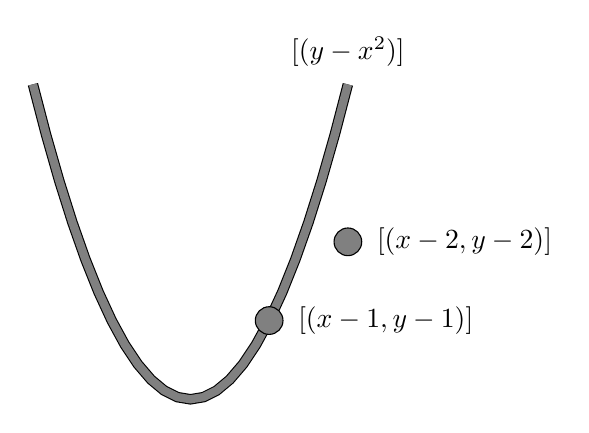
\begin{tikzpicture}
				            \draw[double=gray, double distance=3pt, domain = -2:2, variable = \x]
				            plot ({\x},{\x*\x})
				            node[above=3pt] {$[(y-x^2)]$};

				            \fill[gray!!80] (1,1) circle[radius=5pt];
				            \draw (1,1)
				            circle[radius=5pt]
				            node[right=7pt] {$[(x-1,y-1)]$};

				            \fill[gray!!80] (2,2) circle[radius=5pt];
				            \draw (2,2)
				            circle[radius=5pt]
				            node[right=7pt] {$[(x-2,y-2)]$};
			            \end{tikzpicture}
		            \end{center}

		      \item The associated point $[(x-1,y-1)]$ is embedded in
		            $[(y-x^2)]$, so it is non-reduced. The non-embedded points
		            $[(y-x^2)]$ and $[(x-2,y-2)]$ may or may not be reduced.

		      \item The zerodivisors are precisely those functions that vanish
		            at some associated point, i.e. those that vanish at either
		            $(1,1)$ or $(2,2)$. Hence $x+y-2$ and $y-x^2$ are zerodivisors,
		            but $x+y-3$ is not.
	      \end{enumerate}

	\item If $g\in k[x_1,\ldots,x_n]$ gives a non-trivial zerodivisor in $A$,
	      then we have $gh=rf$ for some $h,r\in k[x_1,\ldots,x_n]$, and
	      $g,h\notin(f)$. Hence every prime factor of $f$ divides either $g$ or
	      $h$, and not all of them divide $h$ (counting with multiplicity) so
	      one of them divides $g$. Say this prime factor is $p$, so we have
	      $f,g\in(p)$ and $(p)$ prime. Then $(p)$ is a minimal prime over $(f)$:
	      if $\p\subsetneq(p)$ then $\p=(p)\cdot\p$, so $\p=0$ since nothing
	      else is infinitely divisible by $p$. Hence $(p)$ is the generic point
	      for an irreducible component of $\Spec A$, and since $g\in(p)$ we get
	      that $g$ vanishes at a non-embedded point.

	      Hence if $[\q]\in\Spec A$ is an associated point, any function
	      vanishing at $[\q]$ also vanishes at some non-embedded associated
	      point. In other words,
	      \begin{equation*}
		      \q \subseteq \bigcup_{\text{non-embedded $\p$}}\p.
	      \end{equation*}
	      This is a finite union because of (B), so by prime avoidance
	      $\q\subseteq\p$ for some non-embedded $\p$. But $\p$ is minimal, so
	      $\q=\p$ is non-embedded.

	\item Suppose $I=\Ann(m)$ and $fg\in I$. Then $\Ann(gm)\supseteq I$, so
	      either $gm=0$ or $\Ann(gm)=I$. In the first case $g\in I$, and in the
	      second case $f\in\Ann(gm)=I$.

	\item If $m\ne0$ then $\Ann(m)$ is proper, and there is a proper ideal
	      containing $\Ann(m)$ maximal among those that are annhilators. By
	      5.5.J this is an associated prime $\p\in\Ass M$, and $m_\p\ne0$ since
	      $\p\supseteq\Ann(m)$.

	\item Since $M'\subseteq M$, we have $\Ass M'\subseteq\Ass M$. Now suppose
	      $m\in M$ has $\Ann(m)=\p\in\Ass M$, and let $m''$ be the image of $m$
	      in $M''$. We have a short exact sequence
	      \begin{equation*}
		      0 \to (A\cdot m)\cap M' \to A\cdot m \to A\cdot m'' \to 0,
	      \end{equation*}
	      so if $(A\cdot m)\cap M'=0$ we get $\p=\Ann(m'')\in\Ass M''$. Otherwise
	      there is some non-zero $x\in (A\cdot m)\cap M'$, and $\Ann(x)=\p$
	      since $A\cdot m\cong A/\p$ is a domain, so $\p\in\Ass M'$.

	\item
	      \begin{enumerate}[label=(\alph*)]
		      \item If no such sequence exists, then $\Ass M$ is non-empty
		            because $M\ne M_0$, so there is a suitable $M_1$, and
		            $\Ass M/M_1$ is non-empty because $M\ne M_1$, so there is a
		            suitable $M_2$, and by induction we get an ascending chain
		            \begin{equation*}
			            0 = M_0 \subsetneq M_1 \subsetneq M_2 \subsetneq \cdots,
		            \end{equation*}
		            contradicting the fact that $M$ is Noetherian.

		      \item By 5.5.L we have
		            \begin{align*}
			            \Ass M & \subseteq \Ass M_{n-1} \cup \Ass A/\p_{n-1}                      \\
			                   & \subseteq \Ass M_{n-2} \cup \Ass A/\p_{n-2} \cup \Ass A/\p_{n-1} \\
			                   & \subseteq \cdots                                                 \\
			                   & \subseteq \Ass A/\p_0 \cup \cdots \cup \Ass A/\p_{n-1}
			            = \{\p_0,\ldots,\p_{n-1}\}.
		            \end{align*}

		      \item We have
		            \begin{equation*}
			            (M_{i+1})_{\p_i} / (M_i)_{\p_i}
			            = (M_{i+1}/M_i)_{\p_i}
			            = K(A/\p_i)
			            \ne 0,
		            \end{equation*}
		            so $(M_{i+1})_{\p_i}\ne0$ and hence $[\p_i]\in\Supp M$. Now
		            since $M$ has a finite generating set $m_1,\ldots,m_n$, we get
		            that $\Supp M=\cup\Supp m_i$ is closed. Therefore
		            $\Supp A/\p_i=\closure{\{[\p_i]\}}\subseteq\Supp M$.
	      \end{enumerate}

	\item As in 5.5.F we have $\Ann_{S^{-1}A}(m/s)=S^{-1}\Ann_A(m)$. Hence
	      \begin{align*}
		      \Ass_{S^{-1}A}S^{-1}M
		       & = \{\text{primes of the form $S^{-1}\Ann_A(m)$}\}                         \\
		       & \leftrightarrow \{\text{primes of the form $\Ann_A(m)$ not meeting $S$}\} \\
		       & = \Ass_AM\cap\Spec S^{-1}A.
	      \end{align*}

	\item Given $[\p]\in\Supp m=V(\Ann m)$, by 5.5.J there is an associated
	      prime of $M_\p$ containing $(\Ann m)_\p$, and by 5.5.N this gives an
	      associated prime $\q\in\Ass M$ with $\Ann m\subseteq\q\subseteq\p$.
	      Hence $\Supp m$ is the closure of $\Ass M\cap\Supp m$.

	      Conversely, any closure of a subset of $\Ass M$ is a finite union
	      $\cup_iV(\p_i)$ of $\p_i=\Ann m_i$, and we may assume
	      $V(\p_i)\not\subseteq V(\p_j)$ for $i\ne j$. If $m=\sum_im_i$, then
	      $\Supp m\subseteq\cup_i\Supp m_i=\cup_iV(\p_i)$, and since
	      $[\p_i]\notin V(\p_j)=\Supp m_j$ we have $m_{\p_j}=(m_j)_{\p_j}\ne0$
	      so $\p_j\in\Supp m$. Hence $\Supp m=\cup_iV(\p_i)$.

	\item
	      \begin{enumerate}[label=(\alph*)]
		      \item Every associated point $\p=\Ann m$ is the generic point of
		            $\Supp m=V(\Ann m)$.

		      \item This was the first paragraph in the solution to 5.5.O.
	      \end{enumerate}

	\item If $X$ is an integral scheme, and $\Spec A\subseteq X$ an affine
	      open subscheme, then $A$ is an integral domain. Hence any $f\in A$ has
	      $\Supp f=V(\Ann f)=V(0)$, so the only associated point of $A$ is the
	      generic point $[(0)]$. Then the only associated point of $X$ is the
	      generic point of $X$, so (B) is immediate. Also (C) follows, since the
	      only zerodivisor is zero, which is the only function vanishing at the
	      generic point.

	\item The irreducible components of $X$ are $V(y-x^2)$ and $V(x-2,y-2)$,
	      so these give the non-embedded associated points. Then the only
	      possible embedded points are $[(x-a,y-a^2)]$ for $a\in\C$. Since $x-1$
	      is a zerodivisor, and $[(x-1,y-1)]$ is the only possible associated
	      point at which it vanishes, we see that $[(x-1,y-1)]$ is an embedded
	      associated point. Now for $a\notin\{1,2\}$ suppose $(x-a)f(x,y)\in I$.
	      Since $y-x^2\ndivides x-a$, we have $f\in(y-x^2)^3$, and since
	      $(x-a)\notin(x-2,y-2)$, we have $f\in(x-2,y-2)$. Also since
	      $(x-a)\notin(x-1,y-1)$, the vanishing order of $f$ at $(1,1)$ must be
	      at least 15. Hence $f(x,y)\in I$, so $x-a$ is not a zerodivisor and
	      $[(x-a,y-a^2)]$ is not an associated point. Finally, the same argument
	      shows that $y-4$ is not a zerodivisor, so $[(x-1,y-1)]$ is the only
	      embedded associated point.
\end{enumerate}

\part{Morphisms}

\chapter{Morphisms of Ringed Spaces}

\begin{enumerate}[label=\textbf{6.2.\Alph*.}]
	\item There is a unique morphism of topological spaces $\pi:X\to Y$ as
	      described, by 2.2.F. Now $\pi_i^{-1}\O_Y=(\pi^{-1}\O_Y)|_{U_i}$, since
	      if $V\subseteq U_i$ we have $\pi_i(V)=\pi(V)$ because
	      $\pi_i=\pi|_{U_i}$. Hence the pullback map for $\pi_i$ is equivalent to
	      a morphism of sheaves $(\pi^{-1}\O_Y)|_{U_i}\to\O_X|_{U_i}$. These
	      morphisms agree when restricted to $U_i\cap U_j$ by assumption, and so
	      since $\shHom(\pi^{-1}\O_Y,\O_X)$ is a sheaf there is a unique morphism
	      of sheaves $\pi^{-1}\O_Y\to\O_X$ that restricts to the pullback
	      $\pi_i^{-1}\O_Y\to\O_X|_{U_i}$ on $U_i$.

	\item The pullback map makes $\O_X(\pi^{-1}(U))$ an $\O_Y(U)$-algebra, and
	      hence $\O_X(\pi^{-1}(U))$-modules become $\O_Y(U)$-modules in a way that
	      preserves morphisms, and this commutes with restriction since the
	      pullback map is a sheaf morphism. In this way an $\O_X$-module
	      $\shMod{M}$ gives an $\O_Y$-module $\pi_*\shMod M$ by
	      $(\pi_*\shMod M)(U)=\shMod M(\pi^{-1}(U))$, and morphisms are preserved
	      so this is a functor $\cat{Mod}_{\O_X}\to\cat{Mod}_{\O_Y}$.

	\item From 2.2.I and 2.3.A we have maps $(\pi_*\O_X)_q\to(\O_X)_p$ and
	      $(\O_Y)_q\to(\pi_*\O_X)_q$.

	\item Firstly note that $\pi^{-1}D(g)=D(\pi^\sharp g)$ because
	      $g\in(\pi^\sharp)^{-1}(\p)$ iff $\pi^\sharp g\in\p$. Now
	      $B_g\to A_{\pi^\sharp g}$ is the localization of $\pi^\sharp$ at $g$ as
	      a map of $B$-algebras, so $A_{\pi^\sharp g}\cong B_g\otimes_BA$. Hence
	      if $D(g)=D(h)$, the unique $B$-algebra isomorphism $B_g\cong B_h$ gives
	      an $A$-algebra isomorphism $A_{\pi^\sharp g}\cong A_{\pi^\sharp h}$ by
	      tensoring with $A$.

	      Moreover this gives a morphism of sheaves on the base, since if
	      $D(f)\subseteq D(g)$ the following square commutes; the vertical map on
	      the right is unique among $A$-algebra morphisms and $(\cdot)\otimes_BA$
	      is functorial.
	      \begin{equation*}
		      \begin{tikzcd}
			      &B_g \arrow{r} \arrow{d}
			      &A_{\pi^\sharp g} \arrow{d} \\
			      &B_f \arrow{r}
			      &A_{\pi^\sharp f}
		      \end{tikzcd}
	      \end{equation*}

	\item As described, we can take the continuous map
	      $\pi:\Spec k(x)\to\Spec k[y]_{(y)}$ with image $[(y)]$, and define a
	      pullback $\O_{\Spec k[y]_{(y)}}\to\pi_*\O_{\Spec k(x)}$ by the obvious
	      map $k[y]_{(y)}\to k(x)$ on global sections, which determines a sheaf
	      morphism since $\pi_*\O_{\Spec k(x)}$ has zero non-global sections,
	      making $\pi$ a morphism of ringed spaces. If this were to come from a
	      ring map $k[y]_{(y)}\to k(x)$ as in 6.2.D, then that ring map must be
	      given by the map on global sections. But the obvious map
	      $k[y]_{(y)}\to k(x)$ does not pull $(0)$ back to $(y)$, so $\pi$ cannot
	      arise in this way.
\end{enumerate}

\begin{enumerate}[label=\textbf{6.3.\Alph*.}]
	\item Using 6.2.A it suffices to show that a morphism of ringed spaces
	      preserves vanishing iff its restrictions to an open cover all preserve
	      vanishing. But this is clear, because restricting to an open
	      neighbourhood doesn't affect the map on stalks.

	\item
	      \begin{enumerate}[label=(\alph*)]
		      \item See 4.3.F.

		      \item An element $f/s\in B_\q$ vanishes at $[\q]$ iff $f\in\q$. If
		            $[\q]=\pi([\p])=[(\pi^\sharp)^{-1}(\p)]$, then
		            $\pi^\sharp(f)\in\p$, so the pullback
		            $\pi^\sharp(f)/\pi^\sharp(s)\in A_\p$ vanishes at $[\p]$.
	      \end{enumerate}

	\item Suppose $\pi:X\to Y$ is a morphism of schemes, and
	      we have affine open subschemes $\Spec B\subseteq Y$,
	      $\Spec A\subseteq \pi^{-1}(\Spec B)$.

	      Note that if $f:Z\to W$ is a morphism of (locally) ringed spaces, and we
	      have open sets $U\subseteq Z$, $f(Z)\subseteq V\subseteq W$, then
	      \begin{itemize}
		      \item There is an inclusion morphism $i:U\to Z$, with pullback
		            given by the identity on $i^{-1}\O_Z=\O_Z|_U$.

		      \item Since $f^{-1}\O_W=f^{-1}(\O_W|_V)$, $f$ is also a morphism
		            $Z\to V$, and hence factors through $V\to W$.
	      \end{itemize}

	      Applying this to our situation, we can compose $\pi$ with the inclusion
	      $\Spec A\to X$ to get $\pi|_{\Spec A}:\Spec A\to Y$, and this factors
	      through $\Spec B\to Y$ so in fact we have a morphism
	      $\pi|_{\Spec A}:\Spec A\to\Spec B$. From 6.3.2 this morphism of schemes
	      must be induced by the map $B\to A$ of global sections, and hence $\pi$
	      has the desired property.

	      Conversely, if $\pi$ looks locally like morphisms of affine schemes,
	      either on all affine open subschemes, or just on a fixed cover
	      $X=\cup_i\Spec A_i$, $Y=\cup_i\Spec B_i$ with
	      $\pi(\Spec A_i)\subseteq\Spec B_i$, then $\pi$ will be a morphism of
	      locally ringed spaces by 6.3.B(b) and 6.3.A.

	\item Clearly $\Spec$ gives a functor from the category of rings to the
	      opposite category of affine schemes. Conversely, let $F$ denote the
	      functor in the reverse direction given by taking global function rings,
	      which sends a morphism $\pi:X\to Y$ to the pullback map
	      $\pi^\sharp:\Gamma(Y,\O_Y)\to\Gamma(X,\O_X)$ coming from
	      $\Gamma(Y,\O_Y)\to\Gamma(Y,\pi_*\O_X)=\Gamma(X,\O_X)$. Clearly we have
	      a canonical isomorphism $F\circ\Spec\cong\id$. Conversely, suppose
	      $\phi_X:X\xrightarrow\sim\Spec A_X$ for each affine scheme $X$. Then
	      $\phi_X^{-1}\circ\Spec(\phi_X^\sharp):\Spec F(X)\xrightarrow\sim X$.
	      Given a morphism $\pi:X\to Y$, the following diagram commutes
	      \begin{equation*}
		      \begin{tikzcd}[column sep=huge]
			      &X \arrow{r}{\pi}
			      &Y \\
			      &\Spec(F(X))
			      \arrow{r}{\Spec(\pi^\sharp)}
			      \arrow{u}{\phi_X^{-1}\circ\Spec(\phi_X^\sharp)}
			      &\Spec(F(Y))
			      \arrow[swap]{u}{\phi_Y^{-1}\circ\Spec(\phi_Y^\sharp)}
		      \end{tikzcd}
	      \end{equation*}
	      since
	      \begin{equation*}
		      \Spec(\phi_Y^\sharp)^{-1}\circ\phi_Y
		      \circ\pi\circ
		      \phi_X^{-1}\circ\Spec(\phi_X^\sharp) = \Spec(\pi^\sharp)
	      \end{equation*}
	      by 6.3.2, because the pullback map for the LHS is
	      \begin{equation*}
		      \phi_X^\sharp\circ(\phi_X^\sharp)^{-1}
		      \circ\pi^\sharp\circ
		      \phi_Y^\sharp\circ(\phi_Y^\sharp)^{-1} = \pi^\sharp.
	      \end{equation*}
	      Hence this gives a natural isomorphism $\Spec\circ F\cong\id$. See
	      6.3.4 for a canonical version.

	\item As well as the cover
	      \begin{equation*}
		      \P^n_k = D_{\P^n_k}(x_0)\cup\cdots\cup D_{\P^n_k}(x_n),
	      \end{equation*}
	      we also have
	      \begin{equation*}
		      \A^{n+1}_k\setminus\{\vec0\}
		      = \A^{n+1}_k\setminus V(x_0,\ldots,x_n)
		      = D_{\A^{n+1}_k}(x_0)\cup\cdots\cup D_{\A^{n+1}_k}(x_n).
	      \end{equation*}
	      These affine open subschemes are given by
	      \begin{align*}
		      D_{\A^{n+1}_k}(x_i) & = \Spec k[x_0,\ldots,x_n,1/x_i]    \\
		      D_{\P^n_k}(x_i)     & = \Spec k[x_0/x_i,\ldots,x_n/x_i],
	      \end{align*}
	      so $k[x_0/x_i,\ldots,x_n/x_i]\subseteq k[x_0,\ldots,x_n,1/x_i]$ gives a
	      morphism of schemes $D_{\A^{n+1}_k}(x_i)\to D_{\P^n_k}(x_i)$. On closed
	      points we get
	      $(a_0,\ldots,a_n)\mapsto[a_0/a_i,\ldots,a_n/a_i]=[a_0,\ldots,a_n]$ as
	      expected.

	      The intersections are
	      \begin{align*}
		      D_{\A^{n+1}_k}(x_i)\cap D_{\A^{n+1}_k}(x_j)
		       & = D_{\A^{n+1}_k}(x_ix_j)
		      = \Spec k[x_0,\ldots,x_n,1/x_i,1/x_j] \\
		      D_{\P^n_k}(x_i)\cap D_{\P^n_k}(x_j)
		       & = D_{\P^n_k}(x_ix_j)
		      = \Spec k[x_0/x_i,\ldots,x_n/x_i,x_0/x_j,\ldots,x_n/x_j],
	      \end{align*}
	      which include into $D_{\A^{n+1}_k}(x_i)$ / $D_{\P^n_k}(x_i)$ by
	      \begin{align*}
		      k[x_0,\ldots,x_n,1/x_i]   & \subseteq
		      k[x_0,\ldots,x_n,1/x_i,1/x_j]         \\
		      k[x_0/x_i,\ldots,x_n/x_i] & \subseteq
		      k[x_0/x_i,\ldots,x_n/x_i,x_0/x_j,\ldots,x_n/x_j].
	      \end{align*}
	      Hence the restriction of $D_{\A^{n+1}_k}(x_i)\to D_{\P^n_k}(x_i)$ to
	      $D_{\A^{n+1}_k}(x_i)\cap D_{\A^{n+1}_k}(x_j)$ is given by
	      \begin{equation*}
		      k[x_0/x_i,\ldots,x_n/x_i] \subseteq k[x_0,\ldots,x_n,1/x_i,1/x_j],
	      \end{equation*}
	      which factors through the morphism
	      $D_{\A^{n+1}_k}(x_i)\cap D_{\A^{n+1}_k}(x_j)\to D_{\P^n_k}(x_i)\cap D_{\P^n_k}(x_j)$
	      given by
	      \begin{equation*}
		      k[x_0/x_i,\ldots,x_n/x_i,x_0/x_j,\ldots,x_n/x_j]
		      \subseteq k[x_0,\ldots,x_n,1/x_i,1/x_j].
	      \end{equation*}
	      Since this final morphism is symmetric with respect to $i$ and $j$, we
	      see that $D_{\A^{n+1}_k}(x_i)\to \P^n_k$ and
	      $D_{\A^{n+1}_k}(x_j)\to \P^n_k$ restrict to the same morphism on
	      $D_{\A^{n+1}_k}(x_i)\cap D_{\A^{n+1}_k}(x_j)$. By gluing, we then get a
	      morphism $\A^{n+1}_k\setminus\{\vec0\}\to\P^n_k$.

	\item Let $\phi_i:\Spec B_i\to U_i\subseteq X$ be open immersions covering
	      $X$. We may assume the cover is closed under intersections, by using
	      distinguished open sets.

	      Given $f:A\to\Gamma(X,\O_X)$, we have morphisms
	      $\Spec(\phi_i^\sharp\circ\res_{X,U_i}\circ f)\circ\phi_i^{-1}:U_i\to\Spec A$.
	      If $U_j\subseteq U_i$, then
	      \begin{equation*}
		      \bigl(\Spec(\phi_i^\sharp\circ\res_{X,U_i}\circ f)
		      \circ\phi_i^{-1}\bigr)|_{U_j}
		      = \Spec(\phi_j^\sharp\circ\res_{X,U_j}\circ f)\circ\phi_j^{-1},
	      \end{equation*}
	      because
	      \begin{equation*}
		      \bigl(\Spec(\phi_i^\sharp\circ\res_{X,U_i}\circ f)
		      \circ\phi_i^{-1}\bigr)|_{U_j}\circ\phi_j
		      = \Spec(\phi_j^\sharp\circ\res_{X,U_j}\circ f)
	      \end{equation*}
	      by 6.3.2, since the pullback on global sections for the LHS is
	      \begin{equation*}
		      \phi_j^\sharp\circ\res_{U_i,U_j}\circ(\phi_i^\sharp)^{-1}\circ
		      (\phi_i^\sharp\circ\res_{X,U_i}\circ f)
		      = \phi_j^\sharp\circ\res_{X,U_j}\circ f.
	      \end{equation*}
	      Hence these morphisms agree on overlaps, and by gluing we get a morphism
	      $\pi:X\to\Spec A$. By construction we have
	      $\res_{X,U_i}\circ \pi^\sharp=(\pi|_{U_i})^\sharp=\res_{X,U_i}\circ f$,
	      so $\pi^\sharp=f$. By 6.3.2, the restrictions $\pi|_{U_i}$ are uniquely
	      determined by this property, and it follows that $\pi$ is unique.

	      This shows that the functor $F$ composed with the obvious natural
	      isomorphism $F\circ\Spec\cong\id$ gives a bijection
	      $\Mor(X,\Spec A)\to\Mor(A,F(X))$, and this is natural in both arguments
	      since $F$ is a functor and $F\circ\Spec\cong\id$ is natural. Hence $F$
	      and $\Spec$, which were an equivalence of categories when restricted to
	      affine schemes, are an adjoint pair on schemes in general.

	      % This is claimed to hold for locally ringed spaces in general, with a
	      % harder proof. See 6.3.6, which also poses the question: what's the
	      % situation for general ringed spaces?

	\item Note that having an $A$-algebra structure on $\Gamma(U,\O_X)$ for each
	      $U$ in a way that commutes with restriction is equivalent to having an
	      $A$-algebra structure on $\Gamma(X,\O_X)$, since $\res_{X,U}$ makes
	      $\Gamma(U,\O_X)$ a $\Gamma(X,\O_X)$-algebra. Hence $A$-schemes in the
	      old sense are equivalent to $A$-schemes in the new sense (as objects) by
	      6.3.F.

	      Now a morphism $X\to Y$ respects the $A$-algebra structure on all
	      section rings iff it does on the global section rings, since both the
	      morphism and the $A$-algebra structure commute with restriction. Hence
	      $X\to Y$ is a morphism of $A$-schemes in the old sense iff
	      $\Gamma(Y,\O_Y)\to\Gamma(X,\O_X)$ is a map of $A$-algebras, i.e. it
	      factors $A\to\Gamma(X,\O_X)$ through $A\to\Gamma(X,\O_X)$. By 6.3.F,
	      this is iff $X\to Y$ factors $X\to\Spec A$ through $Y\to\Spec A$, which
	      is the definition of a morphism of $A$-schemes in the new sense.

	\item The maps $A\to((S_\bullet)_f)_0$ for homogeneous $f\in S_+$ agree on
	      intersections $((S_\bullet)_{fg})_0$, as they are just given by
	      composing $A\to S_\bullet$ with the localization maps. Hence we can glue
	      them to get a canonical morphism $\Proj S_\bullet\to\Spec A$.

	\item Clearly $\Spec\Z$ is final in the category of affine schemes, by
	      equivalence with rings. Hence there is a unique morphism
	      $\Spec A\to\Spec\Z$ for any affine open subscheme $\Spec A\subseteq X$.
	      By uniqueness these agree on overlaps, so by gluing we get a unique
	      morphism $X\to\Spec\Z$.

	      In the category of $A$-schemes $\Spec A$ is final essentially by
	      definition. This applies when $A=k$.

	\item
\end{enumerate}

\end{document}
